% Options for packages loaded elsewhere
\PassOptionsToPackage{unicode}{hyperref}
\PassOptionsToPackage{hyphens}{url}
\PassOptionsToPackage{dvipsnames,svgnames*,x11names*}{xcolor}
%
\documentclass[
  8pt,
  ignorenonframetext,
  dvipsnames]{beamer}
\usepackage{pgfpages}
\setbeamertemplate{caption}[numbered]
\setbeamertemplate{caption label separator}{: }
\setbeamercolor{caption name}{fg=normal text.fg}
\beamertemplatenavigationsymbolsempty
% Prevent slide breaks in the middle of a paragraph
\widowpenalties 1 10000
\raggedbottom
\setbeamertemplate{part page}{
  \centering
  \begin{beamercolorbox}[sep=16pt,center]{part title}
    \usebeamerfont{part title}\insertpart\par
  \end{beamercolorbox}
}
\setbeamertemplate{section page}{
  \centering
  \begin{beamercolorbox}[sep=12pt,center]{part title}
    \usebeamerfont{section title}\insertsection\par
  \end{beamercolorbox}
}
\setbeamertemplate{subsection page}{
  \centering
  \begin{beamercolorbox}[sep=8pt,center]{part title}
    \usebeamerfont{subsection title}\insertsubsection\par
  \end{beamercolorbox}
}
\AtBeginPart{
  \frame{\partpage}
}
\AtBeginSection{
  \ifbibliography
  \else
    \frame{\sectionpage}
  \fi
}
\AtBeginSubsection{
  \frame{\subsectionpage}
}
\usepackage{lmodern}
\usepackage{amssymb,amsmath}
\usepackage{ifxetex,ifluatex}
\ifnum 0\ifxetex 1\fi\ifluatex 1\fi=0 % if pdftex
  \usepackage[T1]{fontenc}
  \usepackage[utf8]{inputenc}
  \usepackage{textcomp} % provide euro and other symbols
\else % if luatex or xetex
  \usepackage{unicode-math}
  \defaultfontfeatures{Scale=MatchLowercase}
  \defaultfontfeatures[\rmfamily]{Ligatures=TeX,Scale=1}
\fi
% Use upquote if available, for straight quotes in verbatim environments
\IfFileExists{upquote.sty}{\usepackage{upquote}}{}
\IfFileExists{microtype.sty}{% use microtype if available
  \usepackage[]{microtype}
  \UseMicrotypeSet[protrusion]{basicmath} % disable protrusion for tt fonts
}{}
\makeatletter
\@ifundefined{KOMAClassName}{% if non-KOMA class
  \IfFileExists{parskip.sty}{%
    \usepackage{parskip}
  }{% else
    \setlength{\parindent}{0pt}
    \setlength{\parskip}{6pt plus 2pt minus 1pt}}
}{% if KOMA class
  \KOMAoptions{parskip=half}}
\makeatother
\usepackage{xcolor}
\IfFileExists{xurl.sty}{\usepackage{xurl}}{} % add URL line breaks if available
\IfFileExists{bookmark.sty}{\usepackage{bookmark}}{\usepackage{hyperref}}
\hypersetup{
  pdftitle={Enter the tidyverse: pipes and dplyr},
  colorlinks=true,
  linkcolor=Maroon,
  filecolor=Maroon,
  citecolor=Blue,
  urlcolor=blue,
  pdfcreator={LaTeX via pandoc}}
\urlstyle{same} % disable monospaced font for URLs
\newif\ifbibliography
\usepackage{color}
\usepackage{fancyvrb}
\newcommand{\VerbBar}{|}
\newcommand{\VERB}{\Verb[commandchars=\\\{\}]}
\DefineVerbatimEnvironment{Highlighting}{Verbatim}{commandchars=\\\{\}}
% Add ',fontsize=\small' for more characters per line
\usepackage{framed}
\definecolor{shadecolor}{RGB}{248,248,248}
\newenvironment{Shaded}{\begin{snugshade}}{\end{snugshade}}
\newcommand{\AlertTok}[1]{\textcolor[rgb]{0.94,0.16,0.16}{#1}}
\newcommand{\AnnotationTok}[1]{\textcolor[rgb]{0.56,0.35,0.01}{\textbf{\textit{#1}}}}
\newcommand{\AttributeTok}[1]{\textcolor[rgb]{0.77,0.63,0.00}{#1}}
\newcommand{\BaseNTok}[1]{\textcolor[rgb]{0.00,0.00,0.81}{#1}}
\newcommand{\BuiltInTok}[1]{#1}
\newcommand{\CharTok}[1]{\textcolor[rgb]{0.31,0.60,0.02}{#1}}
\newcommand{\CommentTok}[1]{\textcolor[rgb]{0.56,0.35,0.01}{\textit{#1}}}
\newcommand{\CommentVarTok}[1]{\textcolor[rgb]{0.56,0.35,0.01}{\textbf{\textit{#1}}}}
\newcommand{\ConstantTok}[1]{\textcolor[rgb]{0.00,0.00,0.00}{#1}}
\newcommand{\ControlFlowTok}[1]{\textcolor[rgb]{0.13,0.29,0.53}{\textbf{#1}}}
\newcommand{\DataTypeTok}[1]{\textcolor[rgb]{0.13,0.29,0.53}{#1}}
\newcommand{\DecValTok}[1]{\textcolor[rgb]{0.00,0.00,0.81}{#1}}
\newcommand{\DocumentationTok}[1]{\textcolor[rgb]{0.56,0.35,0.01}{\textbf{\textit{#1}}}}
\newcommand{\ErrorTok}[1]{\textcolor[rgb]{0.64,0.00,0.00}{\textbf{#1}}}
\newcommand{\ExtensionTok}[1]{#1}
\newcommand{\FloatTok}[1]{\textcolor[rgb]{0.00,0.00,0.81}{#1}}
\newcommand{\FunctionTok}[1]{\textcolor[rgb]{0.00,0.00,0.00}{#1}}
\newcommand{\ImportTok}[1]{#1}
\newcommand{\InformationTok}[1]{\textcolor[rgb]{0.56,0.35,0.01}{\textbf{\textit{#1}}}}
\newcommand{\KeywordTok}[1]{\textcolor[rgb]{0.13,0.29,0.53}{\textbf{#1}}}
\newcommand{\NormalTok}[1]{#1}
\newcommand{\OperatorTok}[1]{\textcolor[rgb]{0.81,0.36,0.00}{\textbf{#1}}}
\newcommand{\OtherTok}[1]{\textcolor[rgb]{0.56,0.35,0.01}{#1}}
\newcommand{\PreprocessorTok}[1]{\textcolor[rgb]{0.56,0.35,0.01}{\textit{#1}}}
\newcommand{\RegionMarkerTok}[1]{#1}
\newcommand{\SpecialCharTok}[1]{\textcolor[rgb]{0.00,0.00,0.00}{#1}}
\newcommand{\SpecialStringTok}[1]{\textcolor[rgb]{0.31,0.60,0.02}{#1}}
\newcommand{\StringTok}[1]{\textcolor[rgb]{0.31,0.60,0.02}{#1}}
\newcommand{\VariableTok}[1]{\textcolor[rgb]{0.00,0.00,0.00}{#1}}
\newcommand{\VerbatimStringTok}[1]{\textcolor[rgb]{0.31,0.60,0.02}{#1}}
\newcommand{\WarningTok}[1]{\textcolor[rgb]{0.56,0.35,0.01}{\textbf{\textit{#1}}}}
\usepackage{longtable,booktabs}
\usepackage{caption}
% Make caption package work with longtable
\makeatletter
\def\fnum@table{\tablename~\thetable}
\makeatother
\usepackage{graphicx}
\makeatletter
\def\maxwidth{\ifdim\Gin@nat@width>\linewidth\linewidth\else\Gin@nat@width\fi}
\def\maxheight{\ifdim\Gin@nat@height>\textheight\textheight\else\Gin@nat@height\fi}
\makeatother
% Scale images if necessary, so that they will not overflow the page
% margins by default, and it is still possible to overwrite the defaults
% using explicit options in \includegraphics[width, height, ...]{}
\setkeys{Gin}{width=\maxwidth,height=\maxheight,keepaspectratio}
% Set default figure placement to htbp
\makeatletter
\def\fps@figure{htbp}
\makeatother
\setlength{\emergencystretch}{3em} % prevent overfull lines
\providecommand{\tightlist}{%
  \setlength{\itemsep}{0pt}\setlength{\parskip}{0pt}}
\setcounter{secnumdepth}{-\maxdimen} % remove section numbering

%packages
\usepackage{graphicx}
\usepackage{rotating}
\usepackage{hyperref}

\usepackage{tikz} % used for text highlighting, amongst others
\usepackage{comment}

%title slide stuff
%\institute{Department of Education}
%\title{Managing and Manipulating Data Using R}

%
\setbeamertemplate{navigation symbols}{} % get rid of navigation icons:
\setbeamertemplate{footline}[page number]

%\setbeamertemplate{frametitle}{\thesection \hspace{0.2cm} \insertframetitle}
\setbeamertemplate{section in toc}[sections numbered]
%\setbeamertemplate{subsection in toc}[subsections numbered]
\setbeamertemplate{subsection in toc}{%
  \leavevmode\leftskip=3.2em\color{gray}\rlap{\hskip-2em\inserttocsectionnumber.\inserttocsubsectionnumber}\inserttocsubsection\par
}

%define colors
%\definecolor{uva_orange}{RGB}{216,141,42} % UVa orange (Rotunda orange)
\definecolor{mygray}{rgb}{0.95, 0.95, 0.95} % for highlighted text
	% grey is equal parts red, green, blue. higher values >> lighter grey
	%\definecolor{lightgraybo}{rgb}{0.83, 0.83, 0.83}

% new commands

%highlight text with very light grey
\newcommand*{\hlg}[1]{%
	\tikz[baseline=(X.base)] \node[rectangle, fill=mygray] (X) {#1};%
}
%, inner sep=0.3mm
%highlight text with very light grey and use font associated with code
\newcommand*{\hlgc}[1]{\texttt{\hlg{#1}}}

%modifying back ticks to add grey background
\let\OldTexttt\texttt
\renewcommand{\texttt}[1]{\OldTexttt{\hlg{#1}}}


\begin{comment}

% Font
\usepackage[defaultfam,light,tabular,lining]{montserrat}
\usepackage[T1]{fontenc}
\renewcommand*\oldstylenums[1]{{\fontfamily{Montserrat-TOsF}\selectfont #1}}

% Change color of boldface text to darkgray
\renewcommand{\textbf}[1]{{\color{darkgray}\bfseries\fontfamily{Montserrat-TOsF}#1}}

% Bullet points
\setbeamertemplate{itemize item}{\color{BlueViolet}$\circ$}
\setbeamertemplate{itemize subitem}{\color{BrickRed}$\triangleright$}
\setbeamertemplate{itemize subsubitem}{$-$}

% Reduce space before lists
%\addtobeamertemplate{itemize/enumerate body begin}{}{\vspace*{-8pt}}

\let\olditem\item
\renewcommand{\item}{%
  \olditem\vspace{4pt}
}

% decreasing space before and after level-2 bullet block
\addtobeamertemplate{itemize/enumerate subbody begin}{}{\vspace*{3pt}}
\addtobeamertemplate{itemize/enumerate subbody end}{}{\vspace*{3pt}}

% decreasing space before and after level-3 bullet block
\addtobeamertemplate{itemize/enumerate subsubbody begin}{}{\vspace*{2pt}}
\addtobeamertemplate{itemize/enumerate subsubbody end}{}{\vspace*{2pt}}

%Section numbering
\setbeamertemplate{section page}{%
    \begingroup
        \begin{beamercolorbox}[sep=10pt,center,rounded=true,shadow=true]{section title}
        \usebeamerfont{section title}\thesection~\insertsection\par
        \end{beamercolorbox}
    \endgroup
}

\setbeamertemplate{subsection page}{%
    \begingroup
        \begin{beamercolorbox}[sep=6pt,center,rounded=true,shadow=true]{subsection title}
        \usebeamerfont{subsection title}\thesection.\thesubsection~\insertsubsection\par
        \end{beamercolorbox}
    \endgroup
}

\end{comment}
\ifluatex
  \usepackage{selnolig}  % disable illegal ligatures
\fi

\title{Enter the tidyverse: pipes and dplyr}
\subtitle{Managing and Manipulating Data Using R}
\author{}
\date{\vspace{-2.5em}}

\begin{document}
\frame{\titlepage}

\begin{frame}{Lecture outline}
\protect\hypertarget{lecture-outline}{}
\tableofcontents
\end{frame}

\hypertarget{introduction}{%
\section{Introduction}\label{introduction}}

\begin{frame}[fragile]{Libraries we will use today}
\protect\hypertarget{libraries-we-will-use-today}{}
``Load'' the package we will use today (output omitted)

\begin{itemize}
\tightlist
\item
  \textbf{you must run this code chunk}
\end{itemize}

\begin{Shaded}
\begin{Highlighting}[]
\KeywordTok{library}\NormalTok{(tidyverse)}
\end{Highlighting}
\end{Shaded}

If package not yet installed, then must install before you load. Install
in ``console'' rather than .Rmd file

\begin{itemize}
\tightlist
\item
  Generic syntax: \texttt{install.packages("package\_name")}
\item
  Install ``tidyverse'': \texttt{install.packages("tidyverse")}
\end{itemize}

Note: when we load package, name of package is not in quotes; but when
we install package, name of package is in quotes:

\begin{itemize}
\tightlist
\item
  \texttt{install.packages("tidyverse")}
\item
  \texttt{library(tidyverse)}
\end{itemize}
\end{frame}

\hypertarget{data-for-lecture-sections-on-select-filter-and-arrange-functions}{%
\subsection{Data for lecture sections on select(), filter(), and
arrange()
functions}\label{data-for-lecture-sections-on-select-filter-and-arrange-functions}}

\begin{frame}[fragile]{Load .Rdata data frames, \texttt{df\_event} and
\texttt{df\_school}}
\protect\hypertarget{load-.rdata-data-frames-df_event-and-df_school}{}
Data on off-campus recruiting events by public universities

\begin{itemize}
\tightlist
\item
  Data frame object \texttt{df\_event}

  \begin{itemize}
  \tightlist
  \item
    One observation per university, recruiting event
  \end{itemize}
\item
  Data frame object \texttt{df\_school}

  \begin{itemize}
  \tightlist
  \item
    One observation per high school (visited and non-visited)
  \end{itemize}
\end{itemize}

\begin{Shaded}
\begin{Highlighting}[]
\KeywordTok{rm}\NormalTok{(}\DataTypeTok{list =} \KeywordTok{ls}\NormalTok{()) }\CommentTok{\# remove all objects in current environment}

\KeywordTok{getwd}\NormalTok{()}
\CommentTok{\#\textgreater{} [1] "/Users/patriciamartin/Desktop/GitHub/rclass1/lectures/enter\_the\_tidyverse"}
\CommentTok{\#load dataset with one obs per recruiting event}
\KeywordTok{load}\NormalTok{(}\KeywordTok{url}\NormalTok{(}\StringTok{"https://github.com/ozanj/rclass/raw/master/data/recruiting/recruit\_event\_somevars.RData"}\NormalTok{))}
\CommentTok{\#load("../../data/recruiting/recruit\_event\_somevars.Rdata")}

\CommentTok{\#load dataset with one obs per high school}
\KeywordTok{load}\NormalTok{(}\KeywordTok{url}\NormalTok{(}\StringTok{"https://github.com/ozanj/rclass/raw/master/data/recruiting/recruit\_school\_somevars.RData"}\NormalTok{))}
\CommentTok{\#load("../../data/recruiting/recruit\_school\_somevars.Rdata")}
\end{Highlighting}
\end{Shaded}
\end{frame}

\hypertarget{data-for-lecture-sections-on-pipes-and-mutate-function}{%
\subsection{Data for lecture sections on pipes and mutate()
function}\label{data-for-lecture-sections-on-pipes-and-mutate-function}}

\begin{frame}[fragile]{Load .Rdata data frame \texttt{wwlist},
``prospects'' purchased by Western Washington U.}
\protect\hypertarget{load-.rdata-data-frame-wwlist-prospects-purchased-by-western-washington-u.}{}
Note: we won't use this data frame until the lecture section on
``pipes''

\begin{itemize}
\tightlist
\item
  You can ignore \texttt{wwlist} data frame for lecture sections on
  select(), filter(), and arrange() functions
\end{itemize}

The ``Student list'' business

\begin{itemize}
\tightlist
\item
  Universities identify/target ``prospects'' by buying ``student lists''
  from College Board/ACT (e.g., \$.40 per prospect)
\item
  Prospect lists contain contact info (e.g., address, email), academic
  achievement, socioeconomic, demographic characteristics
\item
  Universities choose which prospects to purchase by filtering on
  criteria like zip-code, GPA, test score range, etc.
\end{itemize}

\begin{Shaded}
\begin{Highlighting}[]
\CommentTok{\#load prospect list data}
\KeywordTok{load}\NormalTok{(}\KeywordTok{url}\NormalTok{(}\StringTok{"https://github.com/ozanj/rclass/raw/master/data/prospect\_list/wwlist\_merged.RData"}\NormalTok{))}
\end{Highlighting}
\end{Shaded}

Object \texttt{wwlist}

\begin{itemize}
\tightlist
\item
  De-identified list of prospective students purchased by Western
  Washington University from College Board
\item
  We collected these data using public records requests request
\end{itemize}
\end{frame}

\begin{frame}[fragile]{Data frame \texttt{wwlist}, ``prospects''
purchased by Western Washington U.}
\protect\hypertarget{data-frame-wwlist-prospects-purchased-by-western-washington-u.}{}
Observations on \texttt{wwlist}

\begin{itemize}
\tightlist
\item
  each observation represents a prospective student
\end{itemize}

\begin{Shaded}
\begin{Highlighting}[]
\KeywordTok{typeof}\NormalTok{(wwlist)}
\CommentTok{\#\textgreater{} [1] "list"}
\KeywordTok{dim}\NormalTok{(wwlist)}
\CommentTok{\#\textgreater{} [1] 268396     41}
\end{Highlighting}
\end{Shaded}

Variables on \texttt{wwlist}

\begin{itemize}
\tightlist
\item
  some vars provide de-identified data on individual prospects

  \begin{itemize}
  \tightlist
  \item
    e.g., \texttt{psat\_range}, \texttt{state}, \texttt{sex},
    \texttt{ethn\_code}
  \end{itemize}
\item
  some vars provide data about zip-code student lives in

  \begin{itemize}
  \tightlist
  \item
    e.g., \texttt{med\_inc}, \texttt{pop\_total}, \texttt{pop\_black}
  \end{itemize}
\item
  some vars provide data about school student enrolled in

  \begin{itemize}
  \tightlist
  \item
    e.g., \texttt{fr\_lunch} is number of students on free/reduced lunch
  \item
    note: bad merge between prospect-level data and school-level data
  \end{itemize}
\end{itemize}

\begin{Shaded}
\begin{Highlighting}[]
\KeywordTok{names}\NormalTok{(wwlist)}
\KeywordTok{str}\NormalTok{(wwlist)}
\KeywordTok{glimpse}\NormalTok{(wwlist) }\CommentTok{\# tidyverse function, similar to str()}
\end{Highlighting}
\end{Shaded}
\end{frame}

\begin{frame}[fragile]{Data frame \texttt{wwlist}, ``prospects''
purchased by Western Washington U.}
\protect\hypertarget{data-frame-wwlist-prospects-purchased-by-western-washington-u.-1}{}
Variable \texttt{firstgen} identifies whether prospect is a
first-generation college student

Imagine we want to isolate all the first-generation prospects

\begin{enumerate}
\tightlist
\item
  Investigate variable type/structure.
\end{enumerate}

\begin{itemize}
\tightlist
\item
  A dichotomous var, but stored as character in \texttt{wwlist}. So must
  use quotes (\texttt{\textquotesingle{}\textquotesingle{}} or
  \texttt{""}) to filter/subset based on values of \texttt{firstgen}
\end{itemize}

\begin{Shaded}
\begin{Highlighting}[]
\KeywordTok{str}\NormalTok{(wwlist}\OperatorTok{$}\NormalTok{firstgen)}
\CommentTok{\#\textgreater{}  chr [1:268396] NA "N" "N" "N" NA "N" "N" "Y" "Y" "N" "N" "N" "N" "N" "N" ...}
\end{Highlighting}
\end{Shaded}

\begin{enumerate}
\setcounter{enumi}{1}
\tightlist
\item
  Create frequency table to identify possible values of
  \texttt{firstgen}
\end{enumerate}

\begin{Shaded}
\begin{Highlighting}[]
\KeywordTok{table}\NormalTok{(wwlist}\OperatorTok{$}\NormalTok{firstgen, }\DataTypeTok{useNA =} \StringTok{"always"}\NormalTok{)}
\CommentTok{\#\textgreater{} }
\CommentTok{\#\textgreater{}      N      Y   \textless{}NA\textgreater{} }
\CommentTok{\#\textgreater{} 193333  65046  10017}
\end{Highlighting}
\end{Shaded}

\begin{enumerate}
\setcounter{enumi}{2}
\tightlist
\item
  Isolate all the first-gen prospects (output omitted)
\end{enumerate}

\begin{Shaded}
\begin{Highlighting}[]
\KeywordTok{filter}\NormalTok{(wwlist, firstgen }\OperatorTok{==}\StringTok{ "Y"}\NormalTok{)}
\end{Highlighting}
\end{Shaded}
\end{frame}

\hypertarget{investigating-data-patterns}{%
\section{Investigating data
patterns}\label{investigating-data-patterns}}

\begin{frame}[fragile]{Introduction to the \texttt{dplyr} library}
\protect\hypertarget{introduction-to-the-dplyr-library}{}
\texttt{dplyr}, a package within the \texttt{tidyverse} suite of
packages, provide tools for manipulating data frames

\begin{itemize}
\tightlist
\item
  Wickham describes functions within \texttt{dplyr} as a set of
  ``verbs'' that fall in the broader categories of \textbf{subsetting},
  \textbf{sorting}, and \textbf{transforming}
\end{itemize}

\begin{longtable}[]{@{}ll@{}}
\toprule
Today & Upcoming weeks\tabularnewline
\midrule
\endhead
\textbf{Subsetting data} & \textbf{Transforming data}\tabularnewline
- \texttt{select()} variables & - \texttt{mutate()} creates new
variables\tabularnewline
- \texttt{filter()} observations & - \texttt{summarize()} calculates
across rows\tabularnewline
\textbf{Sorting data} & - \texttt{group\_by()} to calculate across rows
within groups\tabularnewline
- \texttt{arrange()} &\tabularnewline
\bottomrule
\end{longtable}

All \texttt{dplyr} verbs (i.e., functions) work as follows

\begin{enumerate}
\tightlist
\item
  first argument is a data frame
\item
  subsequent arguments describe what to do with variables and
  observations in data frame

  \begin{itemize}
  \tightlist
  \item
    refer to variable names without quotes
  \end{itemize}
\item
  result of the function is a new data frame
\end{enumerate}
\end{frame}

\hypertarget{select-variables}{%
\subsection{select() variables}\label{select-variables}}

\begin{frame}[fragile]{Select variables using \texttt{select()}
function}
\protect\hypertarget{select-variables-using-select-function}{}
Printing observations is key to investigating data, but datasets often
have hundreds, thousands of variables

\texttt{select()} function selects \textbf{columns} of data (i.e.,
variables) you specify

\begin{itemize}
\tightlist
\item
  first argument is the name of data frame object
\item
  remaining arguments are variable names, which are separated by commas
  and without quotes
\end{itemize}

Without \textbf{assignment} (\texttt{\textless{}-}), \texttt{select()}
by itself simply prints selected vars

\begin{Shaded}
\begin{Highlighting}[]
\CommentTok{\#?select}
\KeywordTok{select}\NormalTok{(df\_event,instnm,event\_date,event\_type,event\_state,med\_inc)}
\CommentTok{\#\textgreater{} \# A tibble: 18,680 x 5}
\CommentTok{\#\textgreater{}    instnm      event\_date event\_type event\_state med\_inc}
\CommentTok{\#\textgreater{}    \textless{}chr\textgreater{}       \textless{}date\textgreater{}     \textless{}chr\textgreater{}      \textless{}chr\textgreater{}         \textless{}dbl\textgreater{}}
\CommentTok{\#\textgreater{}  1 UM Amherst  2017{-}10{-}12 public hs  MA           71714.}
\CommentTok{\#\textgreater{}  2 UM Amherst  2017{-}10{-}04 public hs  MA           89122.}
\CommentTok{\#\textgreater{}  3 UM Amherst  2017{-}10{-}25 public hs  MA           70136.}
\CommentTok{\#\textgreater{}  4 UM Amherst  2017{-}10{-}26 public hs  MA           70136.}
\CommentTok{\#\textgreater{}  5 Stony Brook 2017{-}10{-}02 public hs  MA           71024.}
\CommentTok{\#\textgreater{}  6 USCC        2017{-}09{-}18 private hs MA           71024.}
\CommentTok{\#\textgreater{}  7 UM Amherst  2017{-}09{-}18 private hs MA           71024.}
\CommentTok{\#\textgreater{}  8 UM Amherst  2017{-}09{-}26 public hs  MA           97225 }
\CommentTok{\#\textgreater{}  9 UM Amherst  2017{-}09{-}26 private hs MA           97225 }
\CommentTok{\#\textgreater{} 10 UM Amherst  2017{-}10{-}12 public hs  MA           77800.}
\CommentTok{\#\textgreater{} \# ... with 18,670 more rows}
\end{Highlighting}
\end{Shaded}
\end{frame}

\begin{frame}[fragile]{Select variables using \texttt{select()}
function}
\protect\hypertarget{select-variables-using-select-function-1}{}
Recall that all \texttt{dplyr} functions (e.g., \texttt{select()})
return a new data frame object

\begin{itemize}
\tightlist
\item
  \textbf{type} equals ``list''
\item
  \textbf{length} equals number of vars you select
\end{itemize}

\begin{Shaded}
\begin{Highlighting}[]
\KeywordTok{typeof}\NormalTok{(}\KeywordTok{select}\NormalTok{(df\_event,instnm,event\_date,event\_type,event\_state,med\_inc))}
\CommentTok{\#\textgreater{} [1] "list"}
\KeywordTok{length}\NormalTok{(}\KeywordTok{select}\NormalTok{(df\_event,instnm,event\_date,event\_type,event\_state,med\_inc))}
\CommentTok{\#\textgreater{} [1] 5}
\end{Highlighting}
\end{Shaded}

\texttt{glimpse()}: tidyverse function for viewing data frames

\begin{itemize}
\tightlist
\item
  a cross between \texttt{str()} and simply printing data
\end{itemize}

\begin{Shaded}
\begin{Highlighting}[]
\NormalTok{?glimpse}
\KeywordTok{glimpse}\NormalTok{(df\_event)}
\end{Highlighting}
\end{Shaded}

\texttt{glimpse()} a \texttt{select()} set of variables

\begin{Shaded}
\begin{Highlighting}[]
\KeywordTok{glimpse}\NormalTok{(}\KeywordTok{select}\NormalTok{(df\_event,instnm,event\_date,event\_type,event\_state,med\_inc))}
\CommentTok{\#\textgreater{} Rows: 18,680}
\CommentTok{\#\textgreater{} Columns: 5}
\CommentTok{\#\textgreater{} $ instnm      \textless{}chr\textgreater{} "UM Amherst", "UM Amherst", "UM Amherst", "UM Amherst",...}
\CommentTok{\#\textgreater{} $ event\_date  \textless{}date\textgreater{} 2017{-}10{-}12, 2017{-}10{-}04, 2017{-}10{-}25, 2017{-}10{-}26, 2017{-}1...}
\CommentTok{\#\textgreater{} $ event\_type  \textless{}chr\textgreater{} "public hs", "public hs", "public hs", "public hs", "pu...}
\CommentTok{\#\textgreater{} $ event\_state \textless{}chr\textgreater{} "MA", "MA", "MA", "MA", "MA", "MA", "MA", "MA", "MA", "...}
\CommentTok{\#\textgreater{} $ med\_inc     \textless{}dbl\textgreater{} 71713.5, 89121.5, 70136.5, 70136.5, 71023.5, 71023.5, 7...}
\end{Highlighting}
\end{Shaded}
\end{frame}

\begin{frame}[fragile]{Select variables using \texttt{select()}
function}
\protect\hypertarget{select-variables-using-select-function-2}{}
With \textbf{assignment} (\texttt{\textless{}-}), \texttt{select()}
creates a new object containing only the variables you specify

\begin{Shaded}
\begin{Highlighting}[]
\NormalTok{event\_small \textless{}{-}}\StringTok{ }\KeywordTok{select}\NormalTok{(df\_event,instnm,event\_date,event\_type,event\_state,}
\NormalTok{  med\_inc)}

\KeywordTok{glimpse}\NormalTok{(event\_small)}
\CommentTok{\#\textgreater{} Rows: 18,680}
\CommentTok{\#\textgreater{} Columns: 5}
\CommentTok{\#\textgreater{} $ instnm      \textless{}chr\textgreater{} "UM Amherst", "UM Amherst", "UM Amherst", "UM Amherst",...}
\CommentTok{\#\textgreater{} $ event\_date  \textless{}date\textgreater{} 2017{-}10{-}12, 2017{-}10{-}04, 2017{-}10{-}25, 2017{-}10{-}26, 2017{-}1...}
\CommentTok{\#\textgreater{} $ event\_type  \textless{}chr\textgreater{} "public hs", "public hs", "public hs", "public hs", "pu...}
\CommentTok{\#\textgreater{} $ event\_state \textless{}chr\textgreater{} "MA", "MA", "MA", "MA", "MA", "MA", "MA", "MA", "MA", "...}
\CommentTok{\#\textgreater{} $ med\_inc     \textless{}dbl\textgreater{} 71713.5, 89121.5, 70136.5, 70136.5, 71023.5, 71023.5, 7...}
\end{Highlighting}
\end{Shaded}
\end{frame}

\begin{frame}[fragile]{Select}
\protect\hypertarget{select}{}
\texttt{select()} can use ``helper functions'' \texttt{starts\_with()},
\texttt{contains()}, and \texttt{ends\_with()} to choose columns

\begin{Shaded}
\begin{Highlighting}[]
\NormalTok{?select}
\end{Highlighting}
\end{Shaded}

Example:

\begin{Shaded}
\begin{Highlighting}[]
\CommentTok{\#names(df\_event)}

\KeywordTok{select}\NormalTok{(df\_event,instnm,}\KeywordTok{starts\_with}\NormalTok{(}\StringTok{"event"}\NormalTok{))}
\CommentTok{\#\textgreater{} \# A tibble: 18,680 x 8}
\CommentTok{\#\textgreater{}    instnm event\_date event\_type event\_state event\_inst event\_name}
\CommentTok{\#\textgreater{}    \textless{}chr\textgreater{}  \textless{}date\textgreater{}     \textless{}chr\textgreater{}      \textless{}chr\textgreater{}       \textless{}chr\textgreater{}      \textless{}chr\textgreater{}     }
\CommentTok{\#\textgreater{}  1 UM Am\textasciitilde{} 2017{-}10{-}12 public hs  MA          In{-}State   Amherst{-}P\textasciitilde{}}
\CommentTok{\#\textgreater{}  2 UM Am\textasciitilde{} 2017{-}10{-}04 public hs  MA          In{-}State   Hampshire\textasciitilde{}}
\CommentTok{\#\textgreater{}  3 UM Am\textasciitilde{} 2017{-}10{-}25 public hs  MA          In{-}State   Chicopee \textasciitilde{}}
\CommentTok{\#\textgreater{}  4 UM Am\textasciitilde{} 2017{-}10{-}26 public hs  MA          In{-}State   Chicopee \textasciitilde{}}
\CommentTok{\#\textgreater{}  5 Stony\textasciitilde{} 2017{-}10{-}02 public hs  MA          Out{-}State  Easthampt\textasciitilde{}}
\CommentTok{\#\textgreater{}  6 USCC   2017{-}09{-}18 private hs MA          Out{-}State  Williston\textasciitilde{}}
\CommentTok{\#\textgreater{}  7 UM Am\textasciitilde{} 2017{-}09{-}18 private hs MA          In{-}State   Williston\textasciitilde{}}
\CommentTok{\#\textgreater{}  8 UM Am\textasciitilde{} 2017{-}09{-}26 public hs  MA          In{-}State   Granby Jr\textasciitilde{}}
\CommentTok{\#\textgreater{}  9 UM Am\textasciitilde{} 2017{-}09{-}26 private hs MA          In{-}State   MacDuffie\textasciitilde{}}
\CommentTok{\#\textgreater{} 10 UM Am\textasciitilde{} 2017{-}10{-}12 public hs  MA          In{-}State   Smith Aca\textasciitilde{}}
\CommentTok{\#\textgreater{} \# ... with 18,670 more rows, and 2 more variables: event\_location\_name \textless{}chr\textgreater{},}
\CommentTok{\#\textgreater{} \#   event\_datetime\_start \textless{}dttm\textgreater{}}
\end{Highlighting}
\end{Shaded}
\end{frame}

\begin{frame}[fragile]{Rename variables}
\protect\hypertarget{rename-variables}{}
\texttt{rename()} function renames variables within a data frame object

\medskip Syntax:

\begin{itemize}
\tightlist
\item
  \texttt{rename(obj\_name,\ new\_name\ =\ old\_name,...)} \medskip
\end{itemize}

\begin{Shaded}
\begin{Highlighting}[]
\KeywordTok{rename}\NormalTok{(df\_event, }\DataTypeTok{g12\_offered =}\NormalTok{ g12offered, }
       \DataTypeTok{titlei =}\NormalTok{ titlei\_status\_pub)}
\KeywordTok{names}\NormalTok{(df\_event)}
\end{Highlighting}
\end{Shaded}

Variable names do not change permanently unless we combine rename with
assignment \medskip

\begin{Shaded}
\begin{Highlighting}[]
\NormalTok{rename\_event \textless{}{-}}\StringTok{ }\KeywordTok{rename}\NormalTok{(df\_event, }\DataTypeTok{g12\_offered =}\NormalTok{ g12offered, }\DataTypeTok{titlei =}\NormalTok{ titlei\_status\_pub)}
\KeywordTok{names}\NormalTok{(rename\_event)}
\KeywordTok{rm}\NormalTok{(rename\_event)}
\end{Highlighting}
\end{Shaded}
\end{frame}

\hypertarget{filter-rows}{%
\subsection{filter() rows}\label{filter-rows}}

\begin{frame}[fragile]{The \texttt{filter()} function}
\protect\hypertarget{the-filter-function}{}
\texttt{filter()} allows you to \textbf{select observations} based on
values of variables

\begin{itemize}
\tightlist
\item
  Arguments

  \begin{itemize}
  \tightlist
  \item
    first argument is name of data frame
  \item
    subsequent arguments are \emph{logical expressions} to filter the
    data frame
  \item
    Multiple expressions separated by commas work as \textbf{AND}
    operators (e.g., condtion 1 \texttt{TRUE} AND condition 2
    \texttt{TRUE})
  \end{itemize}
\item
  What is the result of a \texttt{filter()} command?

  \begin{itemize}
  \tightlist
  \item
    \texttt{filter()} returns a data frame consisting of rows where the
    condition is \texttt{TRUE}
  \end{itemize}
\end{itemize}

\begin{Shaded}
\begin{Highlighting}[]
\NormalTok{?filter}
\end{Highlighting}
\end{Shaded}

Example from data frame object \texttt{df\_school}, each obs is a high
school

\begin{itemize}
\tightlist
\item
  Show all obs where the high school received 1 visit from UC Berkeley
  (110635) {[}output omitted{]}
\end{itemize}

\begin{Shaded}
\begin{Highlighting}[]
\KeywordTok{filter}\NormalTok{(df\_school,visits\_by\_}\DecValTok{110635} \OperatorTok{==}\StringTok{ }\DecValTok{1}\NormalTok{)}
\end{Highlighting}
\end{Shaded}

Note that resulting object is list, consisting of obs where condition
\texttt{TRUE}

\begin{Shaded}
\begin{Highlighting}[]
\KeywordTok{nrow}\NormalTok{(df\_school)}
\CommentTok{\#\textgreater{} [1] 21301}
\KeywordTok{nrow}\NormalTok{(}\KeywordTok{filter}\NormalTok{(df\_school,visits\_by\_}\DecValTok{110635} \OperatorTok{==}\StringTok{ }\DecValTok{1}\NormalTok{))}
\CommentTok{\#\textgreater{} [1] 528}
\end{Highlighting}
\end{Shaded}
\end{frame}

\begin{frame}[fragile]{The \texttt{filter()} function, base R
equivalents}
\protect\hypertarget{the-filter-function-base-r-equivalents}{}
\textbf{Task}: Count the number of high schools that received 1 visit
from UC Berkeley.

\bigskip

\textbf{{[}tidyverse{]}} Using \texttt{filter()}:\smallskip

\begin{Shaded}
\begin{Highlighting}[]
\KeywordTok{nrow}\NormalTok{(}\KeywordTok{filter}\NormalTok{(df\_school, visits\_by\_}\DecValTok{110635} \OperatorTok{==}\StringTok{ }\DecValTok{1}\NormalTok{))}
\CommentTok{\#\textgreater{} [1] 528}
\end{Highlighting}
\end{Shaded}

\bigskip

\textbf{{[}base R{]}} Using \texttt{{[}{]}} and \texttt{\$}:\smallskip

\begin{Shaded}
\begin{Highlighting}[]
\KeywordTok{nrow}\NormalTok{(df\_school[df\_school}\OperatorTok{$}\NormalTok{visits\_by\_}\DecValTok{110635} \OperatorTok{==}\StringTok{ }\DecValTok{1}\NormalTok{, ])}
\CommentTok{\#\textgreater{} [1] 528}
\end{Highlighting}
\end{Shaded}

\bigskip

\textbf{{[}base R{]}} Using \texttt{subset()}:\smallskip

\begin{Shaded}
\begin{Highlighting}[]
\KeywordTok{nrow}\NormalTok{(}\KeywordTok{subset}\NormalTok{(df\_school, visits\_by\_}\DecValTok{110635} \OperatorTok{==}\StringTok{ }\DecValTok{1}\NormalTok{))}
\CommentTok{\#\textgreater{} [1] 528}
\end{Highlighting}
\end{Shaded}
\end{frame}

\begin{frame}[fragile]{Filter, character variables}
\protect\hypertarget{filter-character-variables}{}
Use single quotes \texttt{\textquotesingle{}\textquotesingle{}} or
double quotes \texttt{""} to refer to values of character variables

\begin{Shaded}
\begin{Highlighting}[]
\KeywordTok{glimpse}\NormalTok{(}\KeywordTok{select}\NormalTok{(df\_school, school\_type, state\_code))}
\CommentTok{\#\textgreater{} Rows: 21,301}
\CommentTok{\#\textgreater{} Columns: 2}
\CommentTok{\#\textgreater{} $ school\_type \textless{}chr\textgreater{} "public", "public", "public", "public", "public", "publ...}
\CommentTok{\#\textgreater{} $ state\_code  \textless{}chr\textgreater{} "AK", "AK", "AK", "AK", "AK", "AK", "AK", "AK", "AK", "...}
\end{Highlighting}
\end{Shaded}

Identify all private high schools in CA that got 1 visit by particular
universities

\begin{itemize}
\tightlist
\item
  Visited once by UC Berkeley (ID=110635)
\end{itemize}

\begin{Shaded}
\begin{Highlighting}[]
\KeywordTok{filter}\NormalTok{(df\_school,visits\_by\_}\DecValTok{110635} \OperatorTok{==}\StringTok{ }\DecValTok{1}\NormalTok{, school\_type }\OperatorTok{==}\StringTok{ "private"}\NormalTok{, }
\NormalTok{       state\_code }\OperatorTok{==}\StringTok{ "CA"}\NormalTok{)}
\end{Highlighting}
\end{Shaded}

\begin{itemize}
\tightlist
\item
  Visited once by University of Alabama (ID=100751)
\end{itemize}

\begin{Shaded}
\begin{Highlighting}[]
\KeywordTok{filter}\NormalTok{(df\_school,visits\_by\_}\DecValTok{100751} \OperatorTok{==}\StringTok{ }\DecValTok{1}\NormalTok{, school\_type }\OperatorTok{==}\StringTok{ "private"}\NormalTok{, }
\NormalTok{       state\_code }\OperatorTok{==}\StringTok{ "CA"}\NormalTok{) }
\end{Highlighting}
\end{Shaded}

\begin{itemize}
\tightlist
\item
  Visited once by Berkeley and University of Alabama
\end{itemize}

\begin{Shaded}
\begin{Highlighting}[]
\KeywordTok{filter}\NormalTok{(df\_school,visits\_by\_}\DecValTok{100751} \OperatorTok{==}\StringTok{ }\DecValTok{1}\NormalTok{, visits\_by\_}\DecValTok{110635} \OperatorTok{==}\StringTok{ }\DecValTok{1}\NormalTok{, }
\NormalTok{       school\_type }\OperatorTok{==}\StringTok{ "private"}\NormalTok{, state\_code }\OperatorTok{==}\StringTok{ "CA"}\NormalTok{) }
\end{Highlighting}
\end{Shaded}
\end{frame}

\begin{frame}[fragile]{Filter by multiple conditions, base R
equivalents}
\protect\hypertarget{filter-by-multiple-conditions-base-r-equivalents}{}
\textbf{Task}: Count the number of private high schools in CA that
received 1 visit each from UC Berkeley and University of Alabama.

\medskip

\textbf{{[}tidyverse{]}} Using \texttt{filter()}:\smallskip

\begin{Shaded}
\begin{Highlighting}[]
\KeywordTok{nrow}\NormalTok{(}\KeywordTok{filter}\NormalTok{(df\_school, visits\_by\_}\DecValTok{100751} \OperatorTok{==}\StringTok{ }\DecValTok{1}\NormalTok{, visits\_by\_}\DecValTok{110635} \OperatorTok{==}\StringTok{ }\DecValTok{1}\NormalTok{, }
\NormalTok{            school\_type }\OperatorTok{==}\StringTok{ "private"}\NormalTok{, state\_code }\OperatorTok{==}\StringTok{ "CA"}\NormalTok{))}
\CommentTok{\#\textgreater{} [1] 9}
\end{Highlighting}
\end{Shaded}

\medskip

\textbf{{[}base R{]}} Using \texttt{{[}{]}} and \texttt{\$}:\smallskip

\begin{Shaded}
\begin{Highlighting}[]
\KeywordTok{nrow}\NormalTok{(df\_school[df\_school}\OperatorTok{$}\NormalTok{visits\_by\_}\DecValTok{100751} \OperatorTok{==}\StringTok{ }\DecValTok{1} \OperatorTok{\&}
\StringTok{                 }\NormalTok{df\_school}\OperatorTok{$}\NormalTok{visits\_by\_}\DecValTok{110635} \OperatorTok{==}\StringTok{ }\DecValTok{1} \OperatorTok{\&}
\StringTok{                 }\NormalTok{df\_school}\OperatorTok{$}\NormalTok{school\_type }\OperatorTok{==}\StringTok{ "private"} \OperatorTok{\&}
\StringTok{                 }\NormalTok{df\_school}\OperatorTok{$}\NormalTok{state\_code }\OperatorTok{==}\StringTok{ "CA"}\NormalTok{, ])}
\CommentTok{\#\textgreater{} [1] 9}
\end{Highlighting}
\end{Shaded}

\medskip

\textbf{{[}base R{]}} Using \texttt{subset()}:\smallskip

\begin{Shaded}
\begin{Highlighting}[]
\KeywordTok{nrow}\NormalTok{(}\KeywordTok{subset}\NormalTok{(df\_school, visits\_by\_}\DecValTok{100751} \OperatorTok{==}\StringTok{ }\DecValTok{1} \OperatorTok{\&}\StringTok{ }\NormalTok{visits\_by\_}\DecValTok{110635} \OperatorTok{==}\StringTok{ }\DecValTok{1} \OperatorTok{\&}
\StringTok{            }\NormalTok{school\_type }\OperatorTok{==}\StringTok{ "private"} \OperatorTok{\&}\StringTok{ }\NormalTok{state\_code }\OperatorTok{==}\StringTok{ "CA"}\NormalTok{))}
\CommentTok{\#\textgreater{} [1] 9}
\end{Highlighting}
\end{Shaded}
\end{frame}

\begin{frame}[fragile]{Logical operators for comparisons}
\protect\hypertarget{logical-operators-for-comparisons}{}
logical operators useful for: filter obs w/ \texttt{filter()}; create
variables w/ \texttt{mutate()}

\begin{itemize}
\tightlist
\item
  logical operators also work when using Base R functions
\end{itemize}

\begin{longtable}[]{@{}ll@{}}
\toprule
Operator symbol & Operator meaning\tabularnewline
\midrule
\endhead
\texttt{==} & Equal to\tabularnewline
\texttt{!=} & Not equal to\tabularnewline
\texttt{\textgreater{}} & greater than\tabularnewline
\texttt{\textgreater{}=} & greater than or equal to\tabularnewline
\texttt{\textless{}} & less than\tabularnewline
\texttt{\textless{}=} & less than or equal to\tabularnewline
\texttt{\&} & AND\tabularnewline
\texttt{\textbar{}} & OR\tabularnewline
\texttt{\%in} & includes\tabularnewline
\bottomrule
\end{longtable}

\begin{itemize}
\tightlist
\item
  Visualization of ``Boolean'' operators (e.g., AND, OR, AND NOT)
\end{itemize}

\begin{figure}
\centering
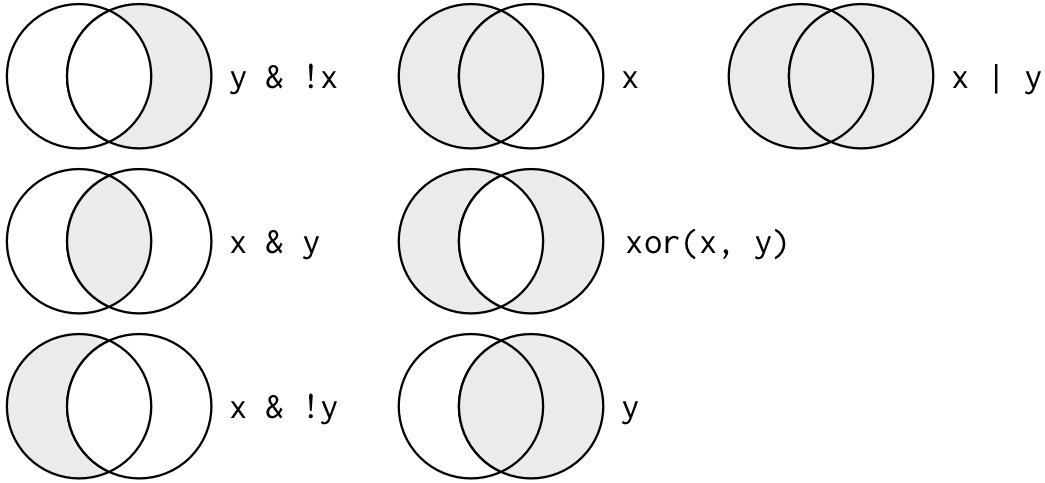
\includegraphics[width=0.4\textwidth,height=\textheight]{transform-logical.png}
\caption{``Boolean'' operations, x=left circle, y=right circle, from
Wichkam (2018)}
\end{figure}
\end{frame}

\begin{frame}[fragile]{Aside: \texttt{count()} function}
\protect\hypertarget{aside-count-function}{}
\medskip \texttt{count()} function from \texttt{dplyr} package counts
the number of obs by group

\textbf{Syntax} {[}see help file for full syntax{]}

\begin{itemize}
\tightlist
\item
  \texttt{count(x,...)}
\end{itemize}

\textbf{Arguments} {[}see help file for full arguments{]}

\begin{itemize}
\tightlist
\item
  \texttt{x}: an object, often a data frame
\item
  \texttt{...}: variables to group by
\end{itemize}

Examples of using \texttt{count()}

\begin{itemize}
\tightlist
\item
  Without vars in \texttt{...} argument, counts number of obs in object
\end{itemize}

\begin{Shaded}
\begin{Highlighting}[]
\KeywordTok{count}\NormalTok{(df\_school)}
  \CommentTok{\# df\_school \%\textgreater{}\% count() \# same as above but using pipes}
\KeywordTok{str}\NormalTok{(}\KeywordTok{count}\NormalTok{(df\_school))}
  \CommentTok{\# \#df\_school \%\textgreater{}\% count() \%\textgreater{}\% str() \# same as above but using pipes}
\end{Highlighting}
\end{Shaded}

\begin{itemize}
\tightlist
\item
  With vars in \texttt{...} argument, counts number of obs per variable
  value

  \begin{itemize}
  \tightlist
  \item
    This is the best way to create frequency table, better than
    \texttt{table()}
  \item
    note: by default, \texttt{count()} always shows \texttt{NAs} {[}this
    is good!{]}
  \end{itemize}
\end{itemize}

\begin{Shaded}
\begin{Highlighting}[]
\KeywordTok{count}\NormalTok{(df\_school,school\_type)}
  \CommentTok{\# df\_school \%\textgreater{}\% count(school\_type) \# same as above but using pipes}
\KeywordTok{str}\NormalTok{(}\KeywordTok{count}\NormalTok{(df\_school,school\_type))}
  \CommentTok{\# df\_school \%\textgreater{}\% count(school\_type) \%\textgreater{}\% str() \# same as above but using pipes}
\end{Highlighting}
\end{Shaded}
\end{frame}

\begin{frame}[fragile]{Filters and comparisons, Demonstration}
\protect\hypertarget{filters-and-comparisons-demonstration}{}
Schools visited by Bama (100751) and/or Berkeley (110635)\bigskip

\begin{Shaded}
\begin{Highlighting}[]
\CommentTok{\# Berkeley AND Bama}
\KeywordTok{filter}\NormalTok{(df\_school,visits\_by\_}\DecValTok{100751} \OperatorTok{\textgreater{}=}\StringTok{ }\DecValTok{1}\NormalTok{, visits\_by\_}\DecValTok{110635} \OperatorTok{\textgreater{}=}\StringTok{ }\DecValTok{1}\NormalTok{) }
\KeywordTok{filter}\NormalTok{(df\_school,visits\_by\_}\DecValTok{100751} \OperatorTok{\textgreater{}=}\StringTok{ }\DecValTok{1} \OperatorTok{\&}\StringTok{ }\NormalTok{visits\_by\_}\DecValTok{110635} \OperatorTok{\textgreater{}=}\StringTok{ }\DecValTok{1}\NormalTok{) }\CommentTok{\# same same}

\NormalTok{df\_school[df\_school}\OperatorTok{$}\NormalTok{visits\_by\_}\DecValTok{100751} \OperatorTok{\textgreater{}=}\StringTok{ }\DecValTok{1} \OperatorTok{\&}
\StringTok{            }\NormalTok{df\_school}\OperatorTok{$}\NormalTok{visits\_by\_}\DecValTok{110635} \OperatorTok{\textgreater{}=}\StringTok{ }\DecValTok{1}\NormalTok{, ] }\CommentTok{\# using [] and $}

\KeywordTok{subset}\NormalTok{(df\_school,visits\_by\_}\DecValTok{100751} \OperatorTok{\textgreater{}=}\StringTok{ }\DecValTok{1} \OperatorTok{\&}
\StringTok{         }\NormalTok{visits\_by\_}\DecValTok{110635} \OperatorTok{\textgreater{}=}\StringTok{ }\DecValTok{1}\NormalTok{) }\CommentTok{\# using subset()}
\end{Highlighting}
\end{Shaded}

\bigskip

\begin{Shaded}
\begin{Highlighting}[]
\CommentTok{\# Berkeley OR Bama}
\KeywordTok{filter}\NormalTok{(df\_school,visits\_by\_}\DecValTok{100751} \OperatorTok{\textgreater{}=}\StringTok{ }\DecValTok{1} \OperatorTok{|}\StringTok{ }\NormalTok{visits\_by\_}\DecValTok{110635} \OperatorTok{\textgreater{}=}\StringTok{ }\DecValTok{1}\NormalTok{)}

\NormalTok{df\_school[df\_school}\OperatorTok{$}\NormalTok{visits\_by\_}\DecValTok{100751} \OperatorTok{\textgreater{}=}\StringTok{ }\DecValTok{1} \OperatorTok{|}
\StringTok{            }\NormalTok{df\_school}\OperatorTok{$}\NormalTok{visits\_by\_}\DecValTok{110635} \OperatorTok{\textgreater{}=}\StringTok{ }\DecValTok{1}\NormalTok{, ] }\CommentTok{\# using [] and $}

\KeywordTok{subset}\NormalTok{(df\_school,visits\_by\_}\DecValTok{100751} \OperatorTok{\textgreater{}=}\StringTok{ }\DecValTok{1} \OperatorTok{|}
\StringTok{         }\NormalTok{visits\_by\_}\DecValTok{110635} \OperatorTok{\textgreater{}=}\StringTok{ }\DecValTok{1}\NormalTok{) }\CommentTok{\# using subset()}
\end{Highlighting}
\end{Shaded}
\end{frame}

\begin{frame}[fragile]{Filters and comparisons, Demonstration (cont.)}
\protect\hypertarget{filters-and-comparisons-demonstration-cont.}{}
Apply \texttt{count()} function on top of \texttt{filter()} function to
count the number of observations that satisfy criteria

\begin{itemize}
\tightlist
\item
  Avoids printing individual observations\medskip
\end{itemize}

\begin{Shaded}
\begin{Highlighting}[]
\CommentTok{\# Number of schools that get visit by Berkeley AND Bama}
\KeywordTok{count}\NormalTok{(}\KeywordTok{filter}\NormalTok{(df\_school, visits\_by\_}\DecValTok{100751} \OperatorTok{\textgreater{}=}\StringTok{ }\DecValTok{1} \OperatorTok{\&}\StringTok{ }\NormalTok{visits\_by\_}\DecValTok{110635} \OperatorTok{\textgreater{}=}\StringTok{ }\DecValTok{1}\NormalTok{))}
\CommentTok{\#\textgreater{} \# A tibble: 1 x 1}
\CommentTok{\#\textgreater{}       n}
\CommentTok{\#\textgreater{}   \textless{}int\textgreater{}}
\CommentTok{\#\textgreater{} 1   247}

\CommentTok{\# Number of schools that get visit by Berkeley OR Bama}
\KeywordTok{count}\NormalTok{(}\KeywordTok{filter}\NormalTok{(df\_school, visits\_by\_}\DecValTok{100751} \OperatorTok{\textgreater{}=}\StringTok{ }\DecValTok{1} \OperatorTok{|}\StringTok{ }\NormalTok{visits\_by\_}\DecValTok{110635} \OperatorTok{\textgreater{}=}\StringTok{ }\DecValTok{1}\NormalTok{))}
\CommentTok{\#\textgreater{} \# A tibble: 1 x 1}
\CommentTok{\#\textgreater{}       n}
\CommentTok{\#\textgreater{}   \textless{}int\textgreater{}}
\CommentTok{\#\textgreater{} 1  2763}
\end{Highlighting}
\end{Shaded}

\begin{itemize}
\tightlist
\item
  Note: You could also use any of the base R equivalents from the
  previous slide
\end{itemize}
\end{frame}

\begin{frame}[fragile]{Filters and comparisons,
\texttt{\textgreater{}=}}
\protect\hypertarget{filters-and-comparisons}{}
Number of public high schools that are at least 50\% Black in Alabama
compared to number of schools that received visit by Bama:\medskip 

\begin{Shaded}
\begin{Highlighting}[]
\CommentTok{\# at least 50\% black}
\KeywordTok{count}\NormalTok{(}\KeywordTok{filter}\NormalTok{(df\_school, school\_type }\OperatorTok{==}\StringTok{ "public"}\NormalTok{, pct\_black }\OperatorTok{\textgreater{}=}\StringTok{ }\DecValTok{50}\NormalTok{, }
\NormalTok{             state\_code }\OperatorTok{==}\StringTok{ "AL"}\NormalTok{))}
\CommentTok{\#\textgreater{} \# A tibble: 1 x 1}
\CommentTok{\#\textgreater{}       n}
\CommentTok{\#\textgreater{}   \textless{}int\textgreater{}}
\CommentTok{\#\textgreater{} 1    86}

\CommentTok{\# at least 50\% black and received visit by Bama}
\KeywordTok{count}\NormalTok{(}\KeywordTok{filter}\NormalTok{(df\_school, school\_type }\OperatorTok{==}\StringTok{ "public"}\NormalTok{, pct\_black }\OperatorTok{\textgreater{}=}\StringTok{ }\DecValTok{50}\NormalTok{, }
\NormalTok{             state\_code }\OperatorTok{==}\StringTok{ "AL"}\NormalTok{, visits\_by\_}\DecValTok{100751} \OperatorTok{\textgreater{}=}\StringTok{ }\DecValTok{1}\NormalTok{))}
\CommentTok{\#\textgreater{} \# A tibble: 1 x 1}
\CommentTok{\#\textgreater{}       n}
\CommentTok{\#\textgreater{}   \textless{}int\textgreater{}}
\CommentTok{\#\textgreater{} 1    21}
\end{Highlighting}
\end{Shaded}
\end{frame}

\begin{frame}[fragile]{Filters and comparisons, \texttt{\textgreater{}=}
(cont.)}
\protect\hypertarget{filters-and-comparisons-cont.}{}
Number of public high schools that are at least 50\% White in Alabama
compared to number of schools that received visit by Bama:\medskip 

\begin{Shaded}
\begin{Highlighting}[]
\CommentTok{\# at least 50\% white}
\KeywordTok{count}\NormalTok{(}\KeywordTok{filter}\NormalTok{(df\_school, school\_type }\OperatorTok{==}\StringTok{ "public"}\NormalTok{, pct\_white }\OperatorTok{\textgreater{}=}\StringTok{ }\DecValTok{50}\NormalTok{, }
\NormalTok{             state\_code }\OperatorTok{==}\StringTok{ "AL"}\NormalTok{))}
\CommentTok{\#\textgreater{} \# A tibble: 1 x 1}
\CommentTok{\#\textgreater{}       n}
\CommentTok{\#\textgreater{}   \textless{}int\textgreater{}}
\CommentTok{\#\textgreater{} 1   238}

\CommentTok{\# at least 50\% white and received visit by Bama}
\KeywordTok{count}\NormalTok{(}\KeywordTok{filter}\NormalTok{(df\_school, school\_type }\OperatorTok{==}\StringTok{ "public"}\NormalTok{, pct\_white }\OperatorTok{\textgreater{}=}\StringTok{ }\DecValTok{50}\NormalTok{, }
\NormalTok{             state\_code }\OperatorTok{==}\StringTok{ "AL"}\NormalTok{, visits\_by\_}\DecValTok{100751} \OperatorTok{\textgreater{}=}\StringTok{ }\DecValTok{1}\NormalTok{))}
\CommentTok{\#\textgreater{} \# A tibble: 1 x 1}
\CommentTok{\#\textgreater{}       n}
\CommentTok{\#\textgreater{}   \textless{}int\textgreater{}}
\CommentTok{\#\textgreater{} 1    82}
\end{Highlighting}
\end{Shaded}
\end{frame}

\begin{frame}[fragile]{Filters and comparisons, not equals
(\texttt{!=})}
\protect\hypertarget{filters-and-comparisons-not-equals}{}
Count the number of high schools visited by University of Colorado
(126614) that are not located in CO

\begin{Shaded}
\begin{Highlighting}[]
\CommentTok{\#number of high schools visited by U Colorado}
\KeywordTok{count}\NormalTok{(}\KeywordTok{filter}\NormalTok{(df\_school, visits\_by\_}\DecValTok{126614} \OperatorTok{\textgreater{}=}\StringTok{ }\DecValTok{1}\NormalTok{))}
\CommentTok{\#\textgreater{} \# A tibble: 1 x 1}
\CommentTok{\#\textgreater{}       n}
\CommentTok{\#\textgreater{}   \textless{}int\textgreater{}}
\CommentTok{\#\textgreater{} 1  1056}

\CommentTok{\#number of high schools visited by U Colorado not located in CO}
\KeywordTok{count}\NormalTok{(}\KeywordTok{filter}\NormalTok{(df\_school, visits\_by\_}\DecValTok{126614} \OperatorTok{\textgreater{}=}\StringTok{ }\DecValTok{1}\NormalTok{, state\_code }\OperatorTok{!=}\StringTok{ "CO"}\NormalTok{))}
\CommentTok{\#\textgreater{} \# A tibble: 1 x 1}
\CommentTok{\#\textgreater{}       n}
\CommentTok{\#\textgreater{}   \textless{}int\textgreater{}}
\CommentTok{\#\textgreater{} 1   873}

\CommentTok{\#number of high schools visited by U Colorado located in CO}
\CommentTok{\#count(filter(df\_school, visits\_by\_126614 \textgreater{}= 1, state\_code == "CO"))}
\end{Highlighting}
\end{Shaded}
\end{frame}

\begin{frame}[fragile]{Filters and comparisons, \texttt{\%in\%}
operator}
\protect\hypertarget{filters-and-comparisons-in-operator}{}
What if you wanted to count the number of schools visited by Bama
(100751) in a group of states?

\begin{Shaded}
\begin{Highlighting}[]
\KeywordTok{count}\NormalTok{(}\KeywordTok{filter}\NormalTok{(df\_school,visits\_by\_}\DecValTok{100751} \OperatorTok{\textgreater{}=}\StringTok{ }\DecValTok{1}\NormalTok{, state\_code }\OperatorTok{==}\StringTok{ "MA"} \OperatorTok{|}
\StringTok{               }\NormalTok{state\_code }\OperatorTok{==}\StringTok{ "VT"} \OperatorTok{|}\StringTok{ }\NormalTok{state\_code }\OperatorTok{==}\StringTok{ "ME"}\NormalTok{))}
\CommentTok{\#\textgreater{} \# A tibble: 1 x 1}
\CommentTok{\#\textgreater{}       n}
\CommentTok{\#\textgreater{}   \textless{}int\textgreater{}}
\CommentTok{\#\textgreater{} 1   108}
\end{Highlighting}
\end{Shaded}

Easier way to do this is with \texttt{\%in\%} operator

\begin{Shaded}
\begin{Highlighting}[]
\KeywordTok{count}\NormalTok{(}\KeywordTok{filter}\NormalTok{(df\_school,visits\_by\_}\DecValTok{100751} \OperatorTok{\textgreater{}=}\StringTok{ }\DecValTok{1}\NormalTok{, state\_code }\OperatorTok{\%in\%}\StringTok{ }\KeywordTok{c}\NormalTok{(}\StringTok{"MA"}\NormalTok{,}\StringTok{"ME"}\NormalTok{,}\StringTok{"VT"}\NormalTok{)))}
\CommentTok{\#\textgreater{} \# A tibble: 1 x 1}
\CommentTok{\#\textgreater{}       n}
\CommentTok{\#\textgreater{}   \textless{}int\textgreater{}}
\CommentTok{\#\textgreater{} 1   108}
\end{Highlighting}
\end{Shaded}

Select the private high schools that got either 2 or 3 visits from Bama

\begin{Shaded}
\begin{Highlighting}[]
\KeywordTok{count}\NormalTok{(}\KeywordTok{filter}\NormalTok{(df\_school, visits\_by\_}\DecValTok{100751} \OperatorTok{\%in\%}\StringTok{ }\DecValTok{2}\OperatorTok{:}\DecValTok{3}\NormalTok{, school\_type }\OperatorTok{==}\StringTok{ "private"}\NormalTok{))}
\CommentTok{\#\textgreater{} \# A tibble: 1 x 1}
\CommentTok{\#\textgreater{}       n}
\CommentTok{\#\textgreater{}   \textless{}int\textgreater{}}
\CommentTok{\#\textgreater{} 1   183}
\end{Highlighting}
\end{Shaded}
\end{frame}

\begin{frame}[fragile]{Identifying data type and possible values helpful
for filtering}
\protect\hypertarget{identifying-data-type-and-possible-values-helpful-for-filtering}{}
\begin{itemize}
\tightlist
\item
  \texttt{typeof()} and \texttt{str()} shows internal data type of a
  variable
\item
  \texttt{table()} to show potential values of categorical variables
\end{itemize}

\begin{Shaded}
\begin{Highlighting}[]
\KeywordTok{typeof}\NormalTok{(df\_event}\OperatorTok{$}\NormalTok{event\_type)}
\CommentTok{\#\textgreater{} [1] "character"}
\KeywordTok{str}\NormalTok{(df\_event}\OperatorTok{$}\NormalTok{event\_type)  }\CommentTok{\# double quotes indicate character}
\CommentTok{\#\textgreater{}  chr [1:18680] "public hs" "public hs" "public hs" "public hs" "public hs" ...}
\KeywordTok{table}\NormalTok{(df\_event}\OperatorTok{$}\NormalTok{event\_type, }\DataTypeTok{useNA=}\StringTok{"always"}\NormalTok{)}
\CommentTok{\#\textgreater{} }
\CommentTok{\#\textgreater{} 2yr college 4yr college       other  private hs   public hs        \textless{}NA\textgreater{} }
\CommentTok{\#\textgreater{}         951         531        2001        3774       11423           0}

\KeywordTok{typeof}\NormalTok{(df\_event}\OperatorTok{$}\NormalTok{med\_inc)}
\CommentTok{\#\textgreater{} [1] "double"}
\KeywordTok{str}\NormalTok{(df\_event}\OperatorTok{$}\NormalTok{med\_inc)}
\CommentTok{\#\textgreater{}  num [1:18680] 71714 89122 70136 70136 71024 ...}
\end{Highlighting}
\end{Shaded}

Now that we know \texttt{event\_type} is a character, we can filter
values

\begin{Shaded}
\begin{Highlighting}[]
\KeywordTok{count}\NormalTok{(}\KeywordTok{filter}\NormalTok{(df\_event, event\_type }\OperatorTok{==}\StringTok{ "public hs"}\NormalTok{, event\_state }\OperatorTok{==}\StringTok{"CA"}\NormalTok{))}
\CommentTok{\#\textgreater{} \# A tibble: 1 x 1}
\CommentTok{\#\textgreater{}       n}
\CommentTok{\#\textgreater{}   \textless{}int\textgreater{}}
\CommentTok{\#\textgreater{} 1  1100}
\CommentTok{\#below code would return an error because variables are character}
\CommentTok{\#count(filter(df\_event, event\_type == public hs, event\_state ==CA))}
\end{Highlighting}
\end{Shaded}
\end{frame}

\begin{frame}[fragile]{Filtering and missing values}
\protect\hypertarget{filtering-and-missing-values}{}
Wickham (2018) states:

\begin{itemize}
\tightlist
\item
  ``\texttt{filter()} only includes rows where condition is TRUE; it
  excludes both \texttt{FALSE} and \texttt{NA} values. To preserve
  missing values, ask for them explicitly:''
\end{itemize}

\medskip Investigate var \texttt{df\_event\$fr\_lunch}, number of
free/reduced lunch students

\begin{itemize}
\tightlist
\item
  only available for visits to public high schools
\end{itemize}

\begin{Shaded}
\begin{Highlighting}[]
\CommentTok{\#visits to public HS with less than 50 students on free/reduced lunch}
\KeywordTok{count}\NormalTok{(}\KeywordTok{filter}\NormalTok{(df\_event,event\_type }\OperatorTok{==}\StringTok{ "public hs"}\NormalTok{, fr\_lunch}\OperatorTok{\textless{}}\DecValTok{50}\NormalTok{))}
\CommentTok{\#\textgreater{} \# A tibble: 1 x 1}
\CommentTok{\#\textgreater{}       n}
\CommentTok{\#\textgreater{}   \textless{}int\textgreater{}}
\CommentTok{\#\textgreater{} 1   910}
\CommentTok{\#visits to public HS, where free/reduced lunch missing}
\KeywordTok{count}\NormalTok{(}\KeywordTok{filter}\NormalTok{(df\_event,event\_type }\OperatorTok{==}\StringTok{ "public hs"}\NormalTok{, }\KeywordTok{is.na}\NormalTok{(fr\_lunch)))}
\CommentTok{\#\textgreater{} \# A tibble: 1 x 1}
\CommentTok{\#\textgreater{}       n}
\CommentTok{\#\textgreater{}   \textless{}int\textgreater{}}
\CommentTok{\#\textgreater{} 1    26}
\CommentTok{\#visits to public HS, where free/reduced is less than 50 OR is missing}
\KeywordTok{count}\NormalTok{(}\KeywordTok{filter}\NormalTok{(df\_event,event\_type }\OperatorTok{==}\StringTok{ "public hs"}\NormalTok{, fr\_lunch}\OperatorTok{\textless{}}\DecValTok{50} \OperatorTok{|}\StringTok{ }\KeywordTok{is.na}\NormalTok{(fr\_lunch)))}
\CommentTok{\#\textgreater{} \# A tibble: 1 x 1}
\CommentTok{\#\textgreater{}       n}
\CommentTok{\#\textgreater{}   \textless{}int\textgreater{}}
\CommentTok{\#\textgreater{} 1   936}
\end{Highlighting}
\end{Shaded}
\end{frame}

\begin{frame}{Exercise}
\protect\hypertarget{exercise}{}
Task

\begin{itemize}
\tightlist
\item
  Create a filter to identify all the high schools that recieved 1 visit
  from UC Berkeley (110635) AND 1 visit from CU Boulder
  (126614){[}output omitted{]}
\end{itemize}
\end{frame}

\begin{frame}[fragile]{Solution}
\protect\hypertarget{solution}{}
\begin{Shaded}
\begin{Highlighting}[]
\KeywordTok{filter}\NormalTok{(df\_school,visits\_by\_}\DecValTok{110635} \OperatorTok{==}\StringTok{ }\DecValTok{1}\NormalTok{, visits\_by\_}\DecValTok{126614}\OperatorTok{==}\DecValTok{1}\NormalTok{)}

\KeywordTok{nrow}\NormalTok{(}\KeywordTok{filter}\NormalTok{(df\_school,visits\_by\_}\DecValTok{110635} \OperatorTok{==}\StringTok{ }\DecValTok{1}\NormalTok{, visits\_by\_}\DecValTok{126614}\OperatorTok{==}\DecValTok{1}\NormalTok{))}
\KeywordTok{count}\NormalTok{(}\KeywordTok{filter}\NormalTok{(df\_school,visits\_by\_}\DecValTok{110635} \OperatorTok{==}\StringTok{ }\DecValTok{1}\NormalTok{, visits\_by\_}\DecValTok{126614}\OperatorTok{==}\DecValTok{1}\NormalTok{))}
\end{Highlighting}
\end{Shaded}

\begin{itemize}
\tightlist
\item
  Must \textbf{assign} to create new object based on filter
\end{itemize}

\begin{Shaded}
\begin{Highlighting}[]
\NormalTok{berk\_boulder \textless{}{-}}\StringTok{ }\KeywordTok{filter}\NormalTok{(df\_school,visits\_by\_}\DecValTok{110635} \OperatorTok{==}\StringTok{ }\DecValTok{1}\NormalTok{, visits\_by\_}\DecValTok{126614}\OperatorTok{==}\DecValTok{1}\NormalTok{)}
\KeywordTok{count}\NormalTok{(berk\_boulder)}
\end{Highlighting}
\end{Shaded}
\end{frame}

\begin{frame}[fragile]{Exercises}
\protect\hypertarget{exercises}{}
Use the data from df\_event, which has one observation for each
off-campus recruiting event a university attends

\begin{enumerate}
\tightlist
\item
  Count the number of events attended by the University of Pittsburgh
  (Pitt) \texttt{univ\_id\ ==\ 215293}\\
\item
  Count the number of recruiting events by Pitt at public or private
  high schools\\
\item
  Count the number of recruiting events by Pitt at public or private
  high schools located in the state of PA\\
\item
  Count the number of recruiting events by Pitt at public high schools
  not located in PA where median income is less than 100,000\\
\item
  Count the number of recruiting events by Pitt at public high schools
  not located in PA where median income is greater than or equal to
  100,000\\
\item
  Count the number of out-of-state recruiting events by Pitt at private
  high schools or public high schools with median income of at least
  100,000
\end{enumerate}
\end{frame}

\begin{frame}[fragile]{Solution}
\protect\hypertarget{solution-1}{}
\begin{enumerate}
\tightlist
\item
  Count the number of events attended by the University of Pittsburgh
  (Pitt) \texttt{univ\_id\ ==\ 215293}
\end{enumerate}

\begin{Shaded}
\begin{Highlighting}[]
\KeywordTok{count}\NormalTok{(}\KeywordTok{filter}\NormalTok{(df\_event, univ\_id }\OperatorTok{==}\StringTok{ }\DecValTok{215293}\NormalTok{))}
\CommentTok{\#\textgreater{} \# A tibble: 1 x 1}
\CommentTok{\#\textgreater{}       n}
\CommentTok{\#\textgreater{}   \textless{}int\textgreater{}}
\CommentTok{\#\textgreater{} 1  1225}
\end{Highlighting}
\end{Shaded}

\begin{enumerate}
\setcounter{enumi}{1}
\tightlist
\item
  Count the number of recruiting events by Pitt at public or private
  high schools
\end{enumerate}

\begin{Shaded}
\begin{Highlighting}[]
\KeywordTok{str}\NormalTok{(df\_event}\OperatorTok{$}\NormalTok{event\_type)}
\CommentTok{\#\textgreater{}  chr [1:18680] "public hs" "public hs" "public hs" "public hs" "public hs" ...}
\KeywordTok{table}\NormalTok{(df\_event}\OperatorTok{$}\NormalTok{event\_type, }\DataTypeTok{useNA =} \StringTok{"always"}\NormalTok{)}
\CommentTok{\#\textgreater{} }
\CommentTok{\#\textgreater{} 2yr college 4yr college       other  private hs   public hs        \textless{}NA\textgreater{} }
\CommentTok{\#\textgreater{}         951         531        2001        3774       11423           0}
\KeywordTok{count}\NormalTok{(}\KeywordTok{filter}\NormalTok{(df\_event, univ\_id }\OperatorTok{==}\StringTok{ }\DecValTok{215293}\NormalTok{, event\_type }\OperatorTok{==}\StringTok{ "private hs"} \OperatorTok{|}
\StringTok{               }\NormalTok{event\_type }\OperatorTok{==}\StringTok{ "public hs"}\NormalTok{))}
\CommentTok{\#\textgreater{} \# A tibble: 1 x 1}
\CommentTok{\#\textgreater{}       n}
\CommentTok{\#\textgreater{}   \textless{}int\textgreater{}}
\CommentTok{\#\textgreater{} 1  1030}
\end{Highlighting}
\end{Shaded}
\end{frame}

\begin{frame}[fragile]{Solution}
\protect\hypertarget{solution-2}{}
\begin{enumerate}
\setcounter{enumi}{2}
\tightlist
\item
  Count the number of recruiting events by Pitt at public or private
  high schools located in the state of PA
\end{enumerate}

\begin{Shaded}
\begin{Highlighting}[]
\KeywordTok{count}\NormalTok{(}\KeywordTok{filter}\NormalTok{(df\_event, univ\_id }\OperatorTok{==}\StringTok{ }\DecValTok{215293}\NormalTok{, event\_type }\OperatorTok{==}\StringTok{ "private hs"} \OperatorTok{|}
\StringTok{               }\NormalTok{event\_type }\OperatorTok{==}\StringTok{ "public hs"}\NormalTok{, event\_state }\OperatorTok{==}\StringTok{ "PA"}\NormalTok{))}
\CommentTok{\#\textgreater{} \# A tibble: 1 x 1}
\CommentTok{\#\textgreater{}       n}
\CommentTok{\#\textgreater{}   \textless{}int\textgreater{}}
\CommentTok{\#\textgreater{} 1   262}
\end{Highlighting}
\end{Shaded}

\begin{enumerate}
\setcounter{enumi}{3}
\tightlist
\item
  Count the number of recruiting events by Pitt at public high schools
  not located in PA where median income is less than 100,000
\end{enumerate}

\begin{Shaded}
\begin{Highlighting}[]
\KeywordTok{count}\NormalTok{(}\KeywordTok{filter}\NormalTok{(df\_event, univ\_id }\OperatorTok{==}\StringTok{ }\DecValTok{215293}\NormalTok{, event\_type }\OperatorTok{==}\StringTok{ "public hs"}\NormalTok{,}
\NormalTok{             event\_state }\OperatorTok{!=}\StringTok{ "PA"}\NormalTok{, med\_inc }\OperatorTok{\textless{}}\StringTok{ }\DecValTok{100000}\NormalTok{))}
\CommentTok{\#\textgreater{} \# A tibble: 1 x 1}
\CommentTok{\#\textgreater{}       n}
\CommentTok{\#\textgreater{}   \textless{}int\textgreater{}}
\CommentTok{\#\textgreater{} 1   213}
\end{Highlighting}
\end{Shaded}
\end{frame}

\begin{frame}[fragile]{Solution}
\protect\hypertarget{solution-3}{}
\begin{enumerate}
\setcounter{enumi}{4}
\tightlist
\item
  Count the number of recruiting events by Pitt at public high schools
  not located in PA where median income is greater than or equal to
  100,000
\end{enumerate}

\begin{Shaded}
\begin{Highlighting}[]
\KeywordTok{count}\NormalTok{(}\KeywordTok{filter}\NormalTok{(df\_event, univ\_id }\OperatorTok{==}\StringTok{ }\DecValTok{215293}\NormalTok{, event\_type }\OperatorTok{==}\StringTok{ "public hs"}\NormalTok{,}
\NormalTok{             event\_state }\OperatorTok{!=}\StringTok{ "PA"}\NormalTok{, med\_inc }\OperatorTok{\textgreater{}=}\StringTok{ }\DecValTok{100000}\NormalTok{))}
\CommentTok{\#\textgreater{} \# A tibble: 1 x 1}
\CommentTok{\#\textgreater{}       n}
\CommentTok{\#\textgreater{}   \textless{}int\textgreater{}}
\CommentTok{\#\textgreater{} 1   344}
\end{Highlighting}
\end{Shaded}

\begin{enumerate}
\setcounter{enumi}{5}
\tightlist
\item
  Count the number of out-of-state recruiting events by Pitt at private
  high schools or public high schools with median income of at least
  100,000
\end{enumerate}

\begin{Shaded}
\begin{Highlighting}[]
\KeywordTok{count}\NormalTok{(}\KeywordTok{filter}\NormalTok{(df\_event, univ\_id }\OperatorTok{==}\StringTok{ }\DecValTok{215293}\NormalTok{, event\_state }\OperatorTok{!=}\StringTok{ "PA"}\NormalTok{, }
\NormalTok{             (event\_type }\OperatorTok{==}\StringTok{ "public hs"} \OperatorTok{\&}\StringTok{ }\NormalTok{med\_inc }\OperatorTok{\textgreater{}=}\StringTok{ }\DecValTok{100000}\NormalTok{) }\OperatorTok{|}
\StringTok{               }\NormalTok{event\_type }\OperatorTok{==}\StringTok{ "private hs"}\NormalTok{))}
\CommentTok{\#\textgreater{} \# A tibble: 1 x 1}
\CommentTok{\#\textgreater{}       n}
\CommentTok{\#\textgreater{}   \textless{}int\textgreater{}}
\CommentTok{\#\textgreater{} 1   553}
\end{Highlighting}
\end{Shaded}
\end{frame}

\hypertarget{arrange-rows-i.e.-sort-rows}{%
\subsection{arrange() rows (i.e., sort
rows)}\label{arrange-rows-i.e.-sort-rows}}

\begin{frame}[fragile]{\texttt{arrange()} function}
\protect\hypertarget{arrange-function}{}
\texttt{arrange()} function ``arranges'' rows in a data frame; said
different, it sorts observations

\medskip

Syntax: \texttt{arrange(x,...)}

\begin{itemize}
\tightlist
\item
  First argument, \texttt{x}, is a data frame
\item
  Subsequent arguments are a ``comma separated list of unquoted variable
  names''
\end{itemize}

\begin{Shaded}
\begin{Highlighting}[]
\KeywordTok{arrange}\NormalTok{(df\_event, event\_date)}
\end{Highlighting}
\end{Shaded}

Data frame goes back to previous order unless you \textbf{assign} the
new order

\begin{Shaded}
\begin{Highlighting}[]
\NormalTok{df\_event}
\NormalTok{df\_event \textless{}{-}}\StringTok{ }\KeywordTok{arrange}\NormalTok{(df\_event, event\_date)}
\NormalTok{df\_event}
\end{Highlighting}
\end{Shaded}
\end{frame}

\begin{frame}[fragile]{\texttt{arrange()} function}
\protect\hypertarget{arrange-function-1}{}
Ascending and descending order

\begin{itemize}
\tightlist
\item
  \texttt{arrange()} sorts in \textbf{ascending} order by default
\item
  use \texttt{desc()} to sort a column by descending order
\end{itemize}

\begin{Shaded}
\begin{Highlighting}[]
\KeywordTok{arrange}\NormalTok{(df\_event, }\KeywordTok{desc}\NormalTok{(event\_date))}
\end{Highlighting}
\end{Shaded}

Can sort by multiple variables

\begin{Shaded}
\begin{Highlighting}[]
\KeywordTok{arrange}\NormalTok{(df\_event, univ\_id, }\KeywordTok{desc}\NormalTok{(event\_date), }\KeywordTok{desc}\NormalTok{(med\_inc))}

\CommentTok{\#sort by university and descending by size of 12th grade class; combine with select}
\KeywordTok{select}\NormalTok{(}\KeywordTok{arrange}\NormalTok{(df\_event, univ\_id, }\KeywordTok{desc}\NormalTok{(g12)),instnm,event\_type,event\_date,g12)}
\end{Highlighting}
\end{Shaded}
\end{frame}

\begin{frame}[fragile]{\texttt{arrange()}, missing values sorted at the
end}
\protect\hypertarget{arrange-missing-values-sorted-at-the-end}{}
Missing values automatically sorted at the end, regardless of whether
you sort ascending or descending

Below, we sort by university, then by date of event, then by ID of high
school

\begin{Shaded}
\begin{Highlighting}[]
\CommentTok{\#by university, date, ascending school id}
\KeywordTok{select}\NormalTok{(}\KeywordTok{arrange}\NormalTok{(df\_event, univ\_id, }\KeywordTok{desc}\NormalTok{(event\_date), school\_id),}
\NormalTok{       instnm,event\_date,event\_type,school\_id)}

\CommentTok{\#by university, date, descending school id}
\KeywordTok{select}\NormalTok{(}\KeywordTok{arrange}\NormalTok{(df\_event, univ\_id, }\KeywordTok{desc}\NormalTok{(event\_date), }\KeywordTok{desc}\NormalTok{(school\_id)),}
\NormalTok{       instnm,event\_date,event\_type,school\_id)}
\end{Highlighting}
\end{Shaded}

Can sort by \texttt{is.na} to put missing values first

\begin{Shaded}
\begin{Highlighting}[]
\KeywordTok{select}\NormalTok{(}\KeywordTok{arrange}\NormalTok{(df\_event, univ\_id, }\KeywordTok{desc}\NormalTok{(event\_date), }\KeywordTok{desc}\NormalTok{(}\KeywordTok{is.na}\NormalTok{(school\_id))),}
\NormalTok{       instnm,event\_date,event\_type,school\_id)}
\CommentTok{\#\textgreater{} \# A tibble: 18,680 x 4}
\CommentTok{\#\textgreater{}    instnm event\_date event\_type school\_id   }
\CommentTok{\#\textgreater{}    \textless{}chr\textgreater{}  \textless{}date\textgreater{}     \textless{}chr\textgreater{}      \textless{}chr\textgreater{}       }
\CommentTok{\#\textgreater{}  1 Bama   2017{-}12{-}18 other      \textless{}NA\textgreater{}        }
\CommentTok{\#\textgreater{}  2 Bama   2017{-}12{-}18 private hs A9106483    }
\CommentTok{\#\textgreater{}  3 Bama   2017{-}12{-}15 other      \textless{}NA\textgreater{}        }
\CommentTok{\#\textgreater{}  4 Bama   2017{-}12{-}15 public hs  484473005095}
\CommentTok{\#\textgreater{}  5 Bama   2017{-}12{-}15 public hs  062927004516}
\CommentTok{\#\textgreater{}  6 Bama   2017{-}12{-}14 other      \textless{}NA\textgreater{}        }
\CommentTok{\#\textgreater{}  7 Bama   2017{-}12{-}13 other      \textless{}NA\textgreater{}        }
\CommentTok{\#\textgreater{}  8 Bama   2017{-}12{-}13 public hs  130387001439}
\CommentTok{\#\textgreater{}  9 Bama   2017{-}12{-}13 private hs 00071151    }
\CommentTok{\#\textgreater{} 10 Bama   2017{-}12{-}13 public hs  063386005296}
\CommentTok{\#\textgreater{} \# ... with 18,670 more rows}
\end{Highlighting}
\end{Shaded}
\end{frame}

\begin{frame}[fragile]{Exercise, arranging}
\protect\hypertarget{exercise-arranging}{}
Use the data from df\_event, which has one observation for each
off-campus recruiting event a university attends

\begin{enumerate}
\tightlist
\item
  Sort ascending by ``univ\_id'' and descending by ``event\_date''\\
\item
  Select four variables in total and sort ascending by ``univ\_id'' and
  descending by ``event\_date''\\
\item
  Now using the same variables from above, sort by \texttt{is.na} to put
  missing values in ``school\_id'' first
\end{enumerate}
\end{frame}

\begin{frame}[fragile]{Solution}
\protect\hypertarget{solution-4}{}
\begin{enumerate}
\tightlist
\item
  Sort ascending by ``univ\_id'' and descending by ``event\_date''
\end{enumerate}

\begin{Shaded}
\begin{Highlighting}[]
\KeywordTok{arrange}\NormalTok{(df\_event, univ\_id, }\KeywordTok{desc}\NormalTok{(event\_date))}
\CommentTok{\#\textgreater{} \# A tibble: 18,680 x 33}
\CommentTok{\#\textgreater{}    instnm univ\_id instst   pid event\_date event\_type zip   school\_id ipeds\_id}
\CommentTok{\#\textgreater{}    \textless{}chr\textgreater{}    \textless{}int\textgreater{} \textless{}chr\textgreater{}  \textless{}int\textgreater{} \textless{}date\textgreater{}     \textless{}chr\textgreater{}      \textless{}chr\textgreater{} \textless{}chr\textgreater{}        \textless{}int\textgreater{}}
\CommentTok{\#\textgreater{}  1 Bama    100751 AL      7115 2017{-}12{-}18 private hs 77089 A9106483        NA}
\CommentTok{\#\textgreater{}  2 Bama    100751 AL      7121 2017{-}12{-}18 other      \textless{}NA\textgreater{}  \textless{}NA\textgreater{}            NA}
\CommentTok{\#\textgreater{}  3 Bama    100751 AL      7114 2017{-}12{-}15 public hs  75165 48447300\textasciitilde{}       NA}
\CommentTok{\#\textgreater{}  4 Bama    100751 AL      7100 2017{-}12{-}15 public hs  93012 06292700\textasciitilde{}       NA}
\CommentTok{\#\textgreater{}  5 Bama    100751 AL      7073 2017{-}12{-}15 other      98027 \textless{}NA\textgreater{}            NA}
\CommentTok{\#\textgreater{}  6 Bama    100751 AL      7072 2017{-}12{-}14 other      98007 \textless{}NA\textgreater{}            NA}
\CommentTok{\#\textgreater{}  7 Bama    100751 AL      7118 2017{-}12{-}13 public hs  31906 13038700\textasciitilde{}       NA}
\CommentTok{\#\textgreater{}  8 Bama    100751 AL      7099 2017{-}12{-}13 private hs 90293 00071151        NA}
\CommentTok{\#\textgreater{}  9 Bama    100751 AL      7109 2017{-}12{-}13 public hs  92630 06338600\textasciitilde{}       NA}
\CommentTok{\#\textgreater{} 10 Bama    100751 AL      7071 2017{-}12{-}13 other      98032 \textless{}NA\textgreater{}            NA}
\CommentTok{\#\textgreater{} \# ... with 18,670 more rows, and 24 more variables: event\_state \textless{}chr\textgreater{},}
\CommentTok{\#\textgreater{} \#   event\_inst \textless{}chr\textgreater{}, med\_inc \textless{}dbl\textgreater{}, pop\_total \textless{}dbl\textgreater{}, pct\_white\_zip \textless{}dbl\textgreater{},}
\CommentTok{\#\textgreater{} \#   pct\_black\_zip \textless{}dbl\textgreater{}, pct\_asian\_zip \textless{}dbl\textgreater{}, pct\_hispanic\_zip \textless{}dbl\textgreater{},}
\CommentTok{\#\textgreater{} \#   pct\_amerindian\_zip \textless{}dbl\textgreater{}, pct\_nativehawaii\_zip \textless{}dbl\textgreater{},}
\CommentTok{\#\textgreater{} \#   pct\_tworaces\_zip \textless{}dbl\textgreater{}, pct\_otherrace\_zip \textless{}dbl\textgreater{}, fr\_lunch \textless{}dbl\textgreater{},}
\CommentTok{\#\textgreater{} \#   titlei\_status\_pub \textless{}fct\textgreater{}, total\_12 \textless{}dbl\textgreater{}, school\_type\_pri \textless{}int\textgreater{},}
\CommentTok{\#\textgreater{} \#   school\_type\_pub \textless{}int\textgreater{}, g12offered \textless{}dbl\textgreater{}, g12 \textless{}dbl\textgreater{},}
\CommentTok{\#\textgreater{} \#   total\_students\_pub \textless{}dbl\textgreater{}, total\_students\_pri \textless{}dbl\textgreater{}, event\_name \textless{}chr\textgreater{},}
\CommentTok{\#\textgreater{} \#   event\_location\_name \textless{}chr\textgreater{}, event\_datetime\_start \textless{}dttm\textgreater{}}
\end{Highlighting}
\end{Shaded}
\end{frame}

\begin{frame}[fragile]{Solution}
\protect\hypertarget{solution-5}{}
\begin{enumerate}
\setcounter{enumi}{1}
\tightlist
\item
  Select four variables in total and sort ascending by ``univ\_id'' and
  descending by ``event\_date''
\end{enumerate}

\begin{Shaded}
\begin{Highlighting}[]
\KeywordTok{select}\NormalTok{(}\KeywordTok{arrange}\NormalTok{(df\_event, univ\_id, }\KeywordTok{desc}\NormalTok{(event\_date)), univ\_id, event\_date, }
\NormalTok{       instnm, event\_type)}
\CommentTok{\#\textgreater{} \# A tibble: 18,680 x 4}
\CommentTok{\#\textgreater{}    univ\_id event\_date instnm event\_type}
\CommentTok{\#\textgreater{}      \textless{}int\textgreater{} \textless{}date\textgreater{}     \textless{}chr\textgreater{}  \textless{}chr\textgreater{}     }
\CommentTok{\#\textgreater{}  1  100751 2017{-}12{-}18 Bama   private hs}
\CommentTok{\#\textgreater{}  2  100751 2017{-}12{-}18 Bama   other     }
\CommentTok{\#\textgreater{}  3  100751 2017{-}12{-}15 Bama   public hs }
\CommentTok{\#\textgreater{}  4  100751 2017{-}12{-}15 Bama   public hs }
\CommentTok{\#\textgreater{}  5  100751 2017{-}12{-}15 Bama   other     }
\CommentTok{\#\textgreater{}  6  100751 2017{-}12{-}14 Bama   other     }
\CommentTok{\#\textgreater{}  7  100751 2017{-}12{-}13 Bama   public hs }
\CommentTok{\#\textgreater{}  8  100751 2017{-}12{-}13 Bama   private hs}
\CommentTok{\#\textgreater{}  9  100751 2017{-}12{-}13 Bama   public hs }
\CommentTok{\#\textgreater{} 10  100751 2017{-}12{-}13 Bama   other     }
\CommentTok{\#\textgreater{} \# ... with 18,670 more rows}
\end{Highlighting}
\end{Shaded}
\end{frame}

\begin{frame}[fragile]{Solution}
\protect\hypertarget{solution-6}{}
\begin{enumerate}
\setcounter{enumi}{2}
\tightlist
\item
  Select the variables ``univ\_id'', ``event\_date'', and ``school\_id''
  and sort by \texttt{is.na} to put missing values in ``school\_id''
  first.
\end{enumerate}

\begin{Shaded}
\begin{Highlighting}[]
\KeywordTok{select}\NormalTok{(}\KeywordTok{arrange}\NormalTok{(df\_event, univ\_id, }\KeywordTok{desc}\NormalTok{(event\_date), }\KeywordTok{desc}\NormalTok{(}\KeywordTok{is.na}\NormalTok{(school\_id))), }
\NormalTok{       univ\_id, event\_date, school\_id)}
\CommentTok{\#\textgreater{} \# A tibble: 18,680 x 3}
\CommentTok{\#\textgreater{}    univ\_id event\_date school\_id   }
\CommentTok{\#\textgreater{}      \textless{}int\textgreater{} \textless{}date\textgreater{}     \textless{}chr\textgreater{}       }
\CommentTok{\#\textgreater{}  1  100751 2017{-}12{-}18 \textless{}NA\textgreater{}        }
\CommentTok{\#\textgreater{}  2  100751 2017{-}12{-}18 A9106483    }
\CommentTok{\#\textgreater{}  3  100751 2017{-}12{-}15 \textless{}NA\textgreater{}        }
\CommentTok{\#\textgreater{}  4  100751 2017{-}12{-}15 484473005095}
\CommentTok{\#\textgreater{}  5  100751 2017{-}12{-}15 062927004516}
\CommentTok{\#\textgreater{}  6  100751 2017{-}12{-}14 \textless{}NA\textgreater{}        }
\CommentTok{\#\textgreater{}  7  100751 2017{-}12{-}13 \textless{}NA\textgreater{}        }
\CommentTok{\#\textgreater{}  8  100751 2017{-}12{-}13 130387001439}
\CommentTok{\#\textgreater{}  9  100751 2017{-}12{-}13 00071151    }
\CommentTok{\#\textgreater{} 10  100751 2017{-}12{-}13 063386005296}
\CommentTok{\#\textgreater{} \# ... with 18,670 more rows}
\end{Highlighting}
\end{Shaded}
\end{frame}

\hypertarget{pipes}{%
\section{Pipes}\label{pipes}}

\begin{frame}[fragile]{What are ``pipes'', \%\textgreater\%}
\protect\hypertarget{what-are-pipes}{}
\textbf{Pipes} are a means of performing multiple steps in a single line
of code

\begin{itemize}
\tightlist
\item
  When writing code, the pipe symbol is \texttt{\%\textgreater{}\%}
\item
  Basic flow of using pipes in code:

  \begin{itemize}
  \tightlist
  \item
    \texttt{object\ \%\textgreater{}\%\ some\_function\ \%\textgreater{}\%\ some\_function\ \%\textgreater{}\%\ some\_function}~\\
  \end{itemize}
\item
  Pipes work from left to right:

  \begin{itemize}
  \tightlist
  \item
    The object from left of \texttt{\%\textgreater{}\%} pipe symbol is
    input as the first argument of the function to the right of the
    \texttt{\%\textgreater{}\%} pipe symbol
  \item
    In turn, the resulting output becomes the input (the first argument)
    of the function to the right of the next \texttt{\%\textgreater{}\%}
    pipe symbol
  \end{itemize}
\item
  Pipes are part of \textbf{tidyverse} suite of packages, not
  \textbf{base R}
\end{itemize}

\medskip

Intuitive mnemonic device for understanding pipes

\begin{itemize}
\tightlist
\item
  whenever you see a pipe \texttt{\%\textgreater{}\%} think of the words
  ``\textbf{and then\ldots{}}''
\end{itemize}

\medskip

Example: isolate all the first-generation prospects {[}output omitted{]}

\begin{itemize}
\tightlist
\item
  in words: start with object \texttt{wwlist} \textbf{and then} filter
  first generation students
\end{itemize}

\begin{Shaded}
\begin{Highlighting}[]
\NormalTok{wwlist }\OperatorTok{\%\textgreater{}\%}\StringTok{ }\KeywordTok{filter}\NormalTok{(firstgen }\OperatorTok{==}\StringTok{ "Y"}\NormalTok{)}
\end{Highlighting}
\end{Shaded}
\end{frame}

\begin{frame}[fragile]{Do task with and without pipes}
\protect\hypertarget{do-task-with-and-without-pipes}{}
Task: Using object \texttt{wwlist} print data for ``first-gen''
prospects (\texttt{firstgen\ ==\ "Y"})

\begin{Shaded}
\begin{Highlighting}[]
\CommentTok{\# without pipes}
\KeywordTok{filter}\NormalTok{(wwlist, firstgen }\OperatorTok{==}\StringTok{ "Y"}\NormalTok{)}

\CommentTok{\# with pipes}
\NormalTok{wwlist }\OperatorTok{\%\textgreater{}\%}\StringTok{ }\KeywordTok{filter}\NormalTok{(firstgen }\OperatorTok{==}\StringTok{ "Y"}\NormalTok{)}
\end{Highlighting}
\end{Shaded}

Comparing the two approaches:

\begin{itemize}
\tightlist
\item
  ``without pipes'', object \texttt{wwlist} is the first argument
  \texttt{filter()} function
\item
  In ``pipes'' approach, you don't specify object \texttt{wwlist} as
  first argument in \texttt{filter()}

  \begin{itemize}
  \tightlist
  \item
    Why? Because \texttt{\%\textgreater{}\%} ``pipes'' the object to the
    left of the \texttt{\%\textgreater{}\%} operator into the function
    to the right of the \texttt{\%\textgreater{}\%} operator
  \end{itemize}
\end{itemize}

Main takeaway:

\begin{itemize}
\tightlist
\item
  When writing code using pipes, functions to right of
  \texttt{\%\textgreater{}\%} pipe operator should not explicitly name
  object that is the input to the function.
\item
  Rather, object to the left of \texttt{\%\textgreater{}\%} pipe
  operator is automatically the input.
\end{itemize}
\end{frame}

\begin{frame}[fragile]{More intuition on the pipe operator,
\texttt{\%\textgreater{}\%}}
\protect\hypertarget{more-intuition-on-the-pipe-operator}{}
The pipe operator ``pipes'' (verb) an object from left of
\texttt{\%\textgreater{}\%} operator into the function to the right of
the \%\textgreater\% operator

Example, the ``structure'' function \texttt{str()}, with and without
pipes

\begin{itemize}
\tightlist
\item
  Examine syntax for \texttt{str()}: \texttt{str(object,\ ...)}
\end{itemize}

\begin{Shaded}
\begin{Highlighting}[]
\NormalTok{?str}
\end{Highlighting}
\end{Shaded}

\begin{itemize}
\tightlist
\item
  Investigate structure of dataframe \texttt{wwlist} without and with
  pipes
\end{itemize}

\begin{Shaded}
\begin{Highlighting}[]
\KeywordTok{str}\NormalTok{(wwlist) }\CommentTok{\# without pipe}

\NormalTok{wwlist }\OperatorTok{\%\textgreater{}\%}\StringTok{ }\KeywordTok{str}\NormalTok{() }\CommentTok{\# with pipe}
\end{Highlighting}
\end{Shaded}

Questions:

\begin{itemize}
\tightlist
\item
  In the pipes approach, \texttt{wwlist\ \%\textgreater{}\%\ str()}, why
  didn't we need to insert argument values inside \texttt{str()}
\item
  What would happen if we just ran this line of code?
\end{itemize}

\begin{Shaded}
\begin{Highlighting}[]
\KeywordTok{str}\NormalTok{()}
\end{Highlighting}
\end{Shaded}
\end{frame}

\begin{frame}[fragile]{Do task with and without pipes}
\protect\hypertarget{do-task-with-and-without-pipes-1}{}
\textbf{Task}: Using object \texttt{wwlist}, print data for
``first-gen'' prospects for selected variables {[}output omitted{]}

\begin{Shaded}
\begin{Highlighting}[]
\CommentTok{\#Without pipes}
\KeywordTok{select}\NormalTok{(}\KeywordTok{filter}\NormalTok{(wwlist, firstgen }\OperatorTok{==}\StringTok{ "Y"}\NormalTok{), state, hs\_city, sex)}
\CommentTok{\#With pipes}
\NormalTok{wwlist }\OperatorTok{\%\textgreater{}\%}\StringTok{ }\KeywordTok{filter}\NormalTok{(firstgen }\OperatorTok{==}\StringTok{ "Y"}\NormalTok{) }\OperatorTok{\%\textgreater{}\%}\StringTok{ }\KeywordTok{select}\NormalTok{(state, hs\_city, sex)}
\end{Highlighting}
\end{Shaded}

Comparing the two approaches:

\begin{itemize}
\tightlist
\item
  In the ``without pipes'' approach, code is written ``inside out''

  \begin{itemize}
  \tightlist
  \item
    The first step in the task -- identifying the object -- is the
    innermost part of code
  \item
    The last step in task -- selecting variables to print -- is the
    outermost part of code
  \end{itemize}
\item
  In ``pipes'' approach the left-to-right order of code matches how we
  think about the task

  \begin{itemize}
  \tightlist
  \item
    First, we start with an object \textbf{\emph{and then}}
    (\texttt{\%\textgreater{}\%}) we use \texttt{filter()} to isolate
    first-gen students \textbf{\emph{and then}}
    (\texttt{\%\textgreater{}\%}) we select which variables to print
  \end{itemize}
\end{itemize}

\medskip

\textbf{Important}: \texttt{str()} function helpful for understanding
what object is piped in from one function to another

\begin{Shaded}
\begin{Highlighting}[]
\CommentTok{\#object that was "piped" into \textasciigrave{}select()\textasciigrave{} from \textasciigrave{}filter()\textasciigrave{}}
\NormalTok{wwlist }\OperatorTok{\%\textgreater{}\%}\StringTok{ }\KeywordTok{filter}\NormalTok{(firstgen }\OperatorTok{==}\StringTok{ "Y"}\NormalTok{) }\OperatorTok{\%\textgreater{}\%}\StringTok{ }\KeywordTok{str}\NormalTok{()}

\CommentTok{\#object that was created after \textasciigrave{}select()\textasciigrave{} function}
\NormalTok{wwlist }\OperatorTok{\%\textgreater{}\%}\StringTok{ }\KeywordTok{filter}\NormalTok{(firstgen }\OperatorTok{==}\StringTok{ "Y"}\NormalTok{) }\OperatorTok{\%\textgreater{}\%}\StringTok{ }\KeywordTok{select}\NormalTok{(state, hs\_city, sex) }\OperatorTok{\%\textgreater{}\%}\StringTok{ }\KeywordTok{str}\NormalTok{()}
\end{Highlighting}
\end{Shaded}
\end{frame}

\begin{frame}[fragile]{Aside: \texttt{count()} function}
\protect\hypertarget{aside-count-function-1}{}
\medskip \texttt{count()} function from \texttt{dplyr} package counts
the number of obs by group

\textbf{Syntax} {[}see help file for full syntax{]}

\begin{itemize}
\tightlist
\item
  \texttt{count(x,...)}
\end{itemize}

\textbf{Arguments} {[}see help file for full arguments{]}

\begin{itemize}
\tightlist
\item
  \texttt{x}: an object, often a data frame
\item
  \texttt{...}: variables to group by
\end{itemize}

Examples of using \texttt{count()}

\begin{itemize}
\tightlist
\item
  Without vars in \texttt{...} argument, counts number of obs in object
\end{itemize}

\begin{Shaded}
\begin{Highlighting}[]
\KeywordTok{count}\NormalTok{(wwlist)}
\NormalTok{wwlist }\OperatorTok{\%\textgreater{}\%}\StringTok{ }\KeywordTok{count}\NormalTok{()}
\NormalTok{wwlist }\OperatorTok{\%\textgreater{}\%}\StringTok{ }\KeywordTok{count}\NormalTok{() }\OperatorTok{\%\textgreater{}\%}\StringTok{ }\KeywordTok{str}\NormalTok{()}
\end{Highlighting}
\end{Shaded}

\begin{itemize}
\tightlist
\item
  With vars in \texttt{...} argument, counts number of obs per variable
  value

  \begin{itemize}
  \tightlist
  \item
    This is the best way to create frequency table, better than
    \texttt{table()}
  \item
    note: by default, \texttt{count()} always shows \texttt{NAs} {[}this
    is good!{]}
  \end{itemize}
\end{itemize}

\begin{Shaded}
\begin{Highlighting}[]
\KeywordTok{count}\NormalTok{(wwlist,school\_category)}
\NormalTok{wwlist }\OperatorTok{\%\textgreater{}\%}\StringTok{ }\KeywordTok{count}\NormalTok{(school\_category)}
\NormalTok{wwlist }\OperatorTok{\%\textgreater{}\%}\StringTok{ }\KeywordTok{count}\NormalTok{(school\_category) }\OperatorTok{\%\textgreater{}\%}\StringTok{ }\KeywordTok{str}\NormalTok{()}
\end{Highlighting}
\end{Shaded}
\end{frame}

\begin{frame}[fragile]{pipe operators and new lines}
\protect\hypertarget{pipe-operators-and-new-lines}{}
\medskip Often want to insert line breaks to make long line of code more
readable

\begin{itemize}
\tightlist
\item
  When inserting line breaks, \textbf{pipe operator
  \texttt{\%\textgreater{}\%} should be the last thing before a line
  break, not the first thing after a line break}
\end{itemize}

\textbf{This works}

\begin{Shaded}
\begin{Highlighting}[]
\NormalTok{wwlist }\OperatorTok{\%\textgreater{}\%}\StringTok{ }\KeywordTok{filter}\NormalTok{(firstgen }\OperatorTok{==}\StringTok{ "Y"}\NormalTok{) }\OperatorTok{\%\textgreater{}\%}\StringTok{ }
\StringTok{  }\KeywordTok{select}\NormalTok{(state, hs\_city, sex) }\OperatorTok{\%\textgreater{}\%}
\StringTok{  }\KeywordTok{count}\NormalTok{(sex)}
\end{Highlighting}
\end{Shaded}

\textbf{This works too}

\begin{Shaded}
\begin{Highlighting}[]
\NormalTok{wwlist }\OperatorTok{\%\textgreater{}\%}\StringTok{ }\KeywordTok{filter}\NormalTok{(firstgen }\OperatorTok{==}\StringTok{ "Y"}\NormalTok{,}
\NormalTok{                  state }\OperatorTok{!=}\StringTok{ "WA"}\NormalTok{) }\OperatorTok{\%\textgreater{}\%}\StringTok{ }
\StringTok{  }\KeywordTok{select}\NormalTok{(state, hs\_city, sex) }\OperatorTok{\%\textgreater{}\%}
\StringTok{  }\KeywordTok{count}\NormalTok{(sex)}
\end{Highlighting}
\end{Shaded}

\textbf{This doesn't work}

\begin{Shaded}
\begin{Highlighting}[]
\NormalTok{wwlist }\OperatorTok{\%\textgreater{}\%}\StringTok{ }\KeywordTok{filter}\NormalTok{(firstgen }\OperatorTok{==}\StringTok{ "Y"}\NormalTok{) }
  \OperatorTok{\%\textgreater{}\%}\StringTok{ }\KeywordTok{select}\NormalTok{(state, hs\_city, sex) }
  \OperatorTok{\%\textgreater{}\%}\StringTok{ }\KeywordTok{count}\NormalTok{(sex)}
\end{Highlighting}
\end{Shaded}
\end{frame}

\begin{frame}[fragile]{The power of pipes}
\protect\hypertarget{the-power-of-pipes}{}
You might be thinking, ``what's the big deal?''

\textbf{TasK}:

\begin{itemize}
\tightlist
\item
  in one line of code, modify \texttt{wwlist} and create bar chart that
  counts number of prospects purchased by race/ethnicity, separately for
  in-state vs.~out-of-state
\end{itemize}

\begin{Shaded}
\begin{Highlighting}[]
\NormalTok{wwlist }\OperatorTok{\%\textgreater{}\%}\StringTok{  }\KeywordTok{filter}\NormalTok{(}\KeywordTok{is.na}\NormalTok{(state)}\OperatorTok{==}\DecValTok{0}\NormalTok{) }\OperatorTok{\%\textgreater{}\%}\StringTok{ }\CommentTok{\# drop obs where variable state missing}
\StringTok{  }\KeywordTok{mutate}\NormalTok{( }\CommentTok{\# create out{-}of{-}state indicator; create recoded ethnicity var}
    \DataTypeTok{out\_state =} \KeywordTok{as\_factor}\NormalTok{(}\KeywordTok{if\_else}\NormalTok{(state }\OperatorTok{!=}\StringTok{ "WA"}\NormalTok{, }\StringTok{"out{-}of{-}state"}\NormalTok{, }\StringTok{"in{-}state"}\NormalTok{)),}
    \DataTypeTok{ethn\_race =} \KeywordTok{recode}\NormalTok{(ethn\_code,}
      \StringTok{"american indian or alaska native"}\NormalTok{ =}\StringTok{ "nativeam"}\NormalTok{,}
      \StringTok{"asian or native hawaiian or other pacific islander"}\NormalTok{ =}\StringTok{ "api"}\NormalTok{,}
      \StringTok{"black or african american"}\NormalTok{ =}\StringTok{ "black"}\NormalTok{,}
      \StringTok{"cuban"}\NormalTok{ =}\StringTok{ "latinx"}\NormalTok{,}
      \StringTok{"mexican/mexican american"}\NormalTok{ =}\StringTok{ "latinx"}\NormalTok{,}
      \StringTok{"not reported"}\NormalTok{ =}\StringTok{ "not\_reported"}\NormalTok{,}
      \StringTok{"other{-}2 or more"}\NormalTok{ =}\StringTok{ "multirace"}\NormalTok{,}
      \StringTok{"other spanish/hispanic"}\NormalTok{ =}\StringTok{ "latinx"}\NormalTok{,}
      \StringTok{"puerto rican"}\NormalTok{ =}\StringTok{ "latinx"}\NormalTok{,}
      \StringTok{"white"}\NormalTok{ =}\StringTok{ "white"}\NormalTok{)) }\OperatorTok{\%\textgreater{}\%}\StringTok{ }
\StringTok{    }\KeywordTok{group\_by}\NormalTok{(out\_state) }\OperatorTok{\%\textgreater{}\%}\StringTok{ }\CommentTok{\# group\_by "in{-}state" vs. "out{-}of{-}state"}
\StringTok{    }\KeywordTok{count}\NormalTok{(ethn\_race) }\OperatorTok{\%\textgreater{}\%}\StringTok{  }\CommentTok{\# count of number of prospects purchased by race}
\StringTok{    }\KeywordTok{ggplot}\NormalTok{(}\KeywordTok{aes}\NormalTok{(}\DataTypeTok{x=}\NormalTok{ethn\_race, }\DataTypeTok{y=}\NormalTok{n)) }\OperatorTok{+}\StringTok{  }\CommentTok{\# plot}
\StringTok{    }\KeywordTok{ylab}\NormalTok{(}\StringTok{"number of prospects"}\NormalTok{) }\OperatorTok{+}\StringTok{ }\KeywordTok{xlab}\NormalTok{(}\StringTok{"race/ethnicity"}\NormalTok{) }\OperatorTok{+}
\StringTok{    }\KeywordTok{geom\_col}\NormalTok{() }\OperatorTok{+}\StringTok{  }\KeywordTok{coord\_flip}\NormalTok{() }\OperatorTok{+}\StringTok{ }\KeywordTok{facet\_wrap}\NormalTok{(}\OperatorTok{\textasciitilde{}}\StringTok{ }\NormalTok{out\_state) }
\end{Highlighting}
\end{Shaded}
\end{frame}

\begin{frame}[fragile]{The power of pipes}
\protect\hypertarget{the-power-of-pipes-1}{}
\textbf{TasK}:

\begin{itemize}
\tightlist
\item
  in one line of code, modify \texttt{wwlist} and create bar chart of
  median income (in zip-code) of prospects purchased by race/ethnicity,
  separately for in-state vs.~out-of-state
\end{itemize}

\begin{Shaded}
\begin{Highlighting}[]
\NormalTok{wwlist }\OperatorTok{\%\textgreater{}\%}\StringTok{  }\KeywordTok{filter}\NormalTok{(}\KeywordTok{is.na}\NormalTok{(state)}\OperatorTok{==}\DecValTok{0}\NormalTok{) }\OperatorTok{\%\textgreater{}\%}\StringTok{ }\CommentTok{\# drop obs where variable state missing}
\StringTok{  }\KeywordTok{mutate}\NormalTok{( }\CommentTok{\# create out{-}of{-}state indicator; create recoded ethnicity var}
    \DataTypeTok{out\_state =} \KeywordTok{as\_factor}\NormalTok{(}\KeywordTok{if\_else}\NormalTok{(state }\OperatorTok{!=}\StringTok{ "WA"}\NormalTok{, }\StringTok{"out{-}of{-}state"}\NormalTok{, }\StringTok{"in{-}state"}\NormalTok{)),}
    \DataTypeTok{ethn\_race =} \KeywordTok{recode}\NormalTok{(ethn\_code,}
      \StringTok{"american indian or alaska native"}\NormalTok{ =}\StringTok{ "nativeam"}\NormalTok{,}
      \StringTok{"asian or native hawaiian or other pacific islander"}\NormalTok{ =}\StringTok{ "api"}\NormalTok{,}
      \StringTok{"black or african american"}\NormalTok{ =}\StringTok{ "black"}\NormalTok{,}
      \StringTok{"cuban"}\NormalTok{ =}\StringTok{ "latinx"}\NormalTok{,}
      \StringTok{"mexican/mexican american"}\NormalTok{ =}\StringTok{ "latinx"}\NormalTok{,}
      \StringTok{"not reported"}\NormalTok{ =}\StringTok{ "not\_reported"}\NormalTok{,}
      \StringTok{"other{-}2 or more"}\NormalTok{ =}\StringTok{ "multirace"}\NormalTok{,}
      \StringTok{"other spanish/hispanic"}\NormalTok{ =}\StringTok{ "latinx"}\NormalTok{,}
      \StringTok{"puerto rican"}\NormalTok{ =}\StringTok{ "latinx"}\NormalTok{,}
      \StringTok{"white"}\NormalTok{ =}\StringTok{ "white"}\NormalTok{)) }\OperatorTok{\%\textgreater{}\%}\StringTok{ }
\StringTok{    }\KeywordTok{group\_by}\NormalTok{(out\_state, ethn\_race) }\OperatorTok{\%\textgreater{}\%}\StringTok{ }\CommentTok{\# group\_by "out{-}state" and ethnicity}
\StringTok{    }\KeywordTok{summarize}\NormalTok{(}\DataTypeTok{avg\_inc\_zip =} \KeywordTok{mean}\NormalTok{(med\_inc\_zip, }\DataTypeTok{na.rm =} \OtherTok{TRUE}\NormalTok{)) }\OperatorTok{\%\textgreater{}\%}\StringTok{ }\CommentTok{\# calculate avg. inc}
\StringTok{    }\KeywordTok{ggplot}\NormalTok{(}\KeywordTok{aes}\NormalTok{(}\DataTypeTok{x=}\NormalTok{out\_state, }\DataTypeTok{y=}\NormalTok{avg\_inc\_zip)) }\OperatorTok{+}\StringTok{ }
\StringTok{    }\KeywordTok{ylab}\NormalTok{(}\StringTok{"avg. income in zip code"}\NormalTok{) }\OperatorTok{+}\StringTok{ }\KeywordTok{xlab}\NormalTok{(}\StringTok{""}\NormalTok{) }\OperatorTok{+}
\StringTok{    }\KeywordTok{geom\_col}\NormalTok{() }\OperatorTok{+}\StringTok{  }\KeywordTok{coord\_flip}\NormalTok{() }\OperatorTok{+}\StringTok{ }\KeywordTok{facet\_wrap}\NormalTok{(}\OperatorTok{\textasciitilde{}}\StringTok{ }\NormalTok{ethn\_race) }\CommentTok{\# plot}
\end{Highlighting}
\end{Shaded}
\end{frame}

\begin{frame}{The power of pipes}
\protect\hypertarget{the-power-of-pipes-2}{}
Example R script from Ben Skinner, which creates analysis data for
\href{https://link.springer.com/article/10.1007\%2Fs11162-018-9507-1}{Skinner
(2018)}

\begin{itemize}
\tightlist
\item
  \href{https://github.com/btskinner/colchoice_rep/blob/master/scripts/makedata.r}{Link
  to R script}
\end{itemize}

\medskip

Other relevant links

\begin{itemize}
\tightlist
\item
  \href{https://github.com/btskinner/colchoice_rep}{Link to Github
  repository for Skinner (2018)}
\item
  \href{https://link.springer.com/article/10.1007\%2Fs11162-018-9507-1}{Link
  to published paper}
\item
  \href{https://github.com/btskinner}{Link to Skinner's Github page}

  \begin{itemize}
  \tightlist
  \item
    A lot of cool stuff here
  \end{itemize}
\item
  \href{https://www.btskinner.io/}{Link to Skinner's personal website}

  \begin{itemize}
  \tightlist
  \item
    A lot of cool stuff here
  \end{itemize}
\end{itemize}
\end{frame}

\begin{frame}[fragile]{Do task with and without pipes {[}STUDENTS WORK
ON THEIR OWN{]}}
\protect\hypertarget{do-task-with-and-without-pipes-students-work-on-their-own}{}
Task:

\begin{itemize}
\tightlist
\item
  Count the number ``first-generation'' prospects from the state of
  Washington
\end{itemize}

Without pipes

\begin{Shaded}
\begin{Highlighting}[]
\KeywordTok{count}\NormalTok{(}\KeywordTok{filter}\NormalTok{(wwlist, firstgen }\OperatorTok{==}\StringTok{ "Y"}\NormalTok{, state }\OperatorTok{==}\StringTok{ "WA"}\NormalTok{))}
\CommentTok{\#\textgreater{} \# A tibble: 1 x 1}
\CommentTok{\#\textgreater{}       n}
\CommentTok{\#\textgreater{}   \textless{}int\textgreater{}}
\CommentTok{\#\textgreater{} 1 32428}
\end{Highlighting}
\end{Shaded}

With pipes

\begin{Shaded}
\begin{Highlighting}[]
\NormalTok{wwlist }\OperatorTok{\%\textgreater{}\%}\StringTok{ }\KeywordTok{filter}\NormalTok{(firstgen }\OperatorTok{==}\StringTok{ "Y"}\NormalTok{, state }\OperatorTok{==}\StringTok{ "WA"}\NormalTok{) }\OperatorTok{\%\textgreater{}\%}\StringTok{ }\KeywordTok{count}\NormalTok{()}
\CommentTok{\#\textgreater{} \# A tibble: 1 x 1}
\CommentTok{\#\textgreater{}       n}
\CommentTok{\#\textgreater{}   \textless{}int\textgreater{}}
\CommentTok{\#\textgreater{} 1 32428}
\end{Highlighting}
\end{Shaded}
\end{frame}

\begin{frame}[fragile]{Do task with and without pipes {[}STUDENTS WORK
ON THEIR OWN{]}}
\protect\hypertarget{do-task-with-and-without-pipes-students-work-on-their-own-1}{}
\textbf{Task}: frequency table of \texttt{school\_type} for non
first-gen prospects from WA

\textbf{Without pipes}

\begin{Shaded}
\begin{Highlighting}[]
\NormalTok{wwlist\_temp \textless{}{-}}\StringTok{ }\KeywordTok{filter}\NormalTok{(wwlist, firstgen }\OperatorTok{==}\StringTok{ "N"}\NormalTok{, state }\OperatorTok{==}\StringTok{ "WA"}\NormalTok{)}
\KeywordTok{table}\NormalTok{(wwlist\_temp}\OperatorTok{$}\NormalTok{school\_type, }\DataTypeTok{useNA =} \StringTok{"always"}\NormalTok{)}
\CommentTok{\#\textgreater{} }
\CommentTok{\#\textgreater{} private  public    \textless{}NA\textgreater{} }
\CommentTok{\#\textgreater{}      11   46146   12489}
\KeywordTok{rm}\NormalTok{(wwlist\_temp) }\CommentTok{\# cuz we don\textquotesingle{}t need after creating table}
\end{Highlighting}
\end{Shaded}

\textbf{With pipes}

\begin{Shaded}
\begin{Highlighting}[]
\NormalTok{wwlist }\OperatorTok{\%\textgreater{}\%}\StringTok{ }\KeywordTok{filter}\NormalTok{(firstgen }\OperatorTok{==}\StringTok{ "N"}\NormalTok{, state }\OperatorTok{==}\StringTok{ "WA"}\NormalTok{) }\OperatorTok{\%\textgreater{}\%}\StringTok{ }\KeywordTok{count}\NormalTok{(school\_type)}
\CommentTok{\#\textgreater{} \# A tibble: 3 x 2}
\CommentTok{\#\textgreater{}   school\_type     n}
\CommentTok{\#\textgreater{}   \textless{}chr\textgreater{}       \textless{}int\textgreater{}}
\CommentTok{\#\textgreater{} 1 private        11}
\CommentTok{\#\textgreater{} 2 public      46146}
\CommentTok{\#\textgreater{} 3 \textless{}NA\textgreater{}        12489}
\end{Highlighting}
\end{Shaded}

\textbf{Comparison of two approaches}

\begin{itemize}
\tightlist
\item
  without pipes, task requires multiple lines of code (this is quite
  common)

  \begin{itemize}
  \tightlist
  \item
    first line creates object; second line analyzes object
  \end{itemize}
\item
  with pipes, task can be completed in one line of code and you aren't
  left with objects you don't care about
\end{itemize}
\end{frame}

\begin{frame}[fragile]{Student exercises with pipes}
\protect\hypertarget{student-exercises-with-pipes}{}
\begin{enumerate}
\item
  Using object \texttt{wwlist} select the following variables (state,
  firstgen, ethn\_code) and assign \texttt{\textless{}-} them to object
  \texttt{wwlist\_temp}. (ex. wwlist\_temp \textless- wwlist)
\item
  Using the object you just created \texttt{wwlist\_temp}, create a
  frequency table of \texttt{ethn\_code} for first-gen prospects from
  California.
\item
  \textbf{Bonus}: Try doing question 1 and 2 together. Use original
  object \texttt{wwlist}, but do not assign to a new object.
\end{enumerate}

Once finished you can \texttt{rm(wwlist\_temp)}
\end{frame}

\begin{frame}[fragile]{Solution to exercises with pipes}
\protect\hypertarget{solution-to-exercises-with-pipes}{}
\begin{enumerate}
\tightlist
\item
  Using object \texttt{wwlist} select the following variables (state,
  firstgen, ethn\_code) and assign them to object \texttt{wwlist\_temp}
\end{enumerate}

\begin{Shaded}
\begin{Highlighting}[]
\NormalTok{wwlist\_temp \textless{}{-}}\StringTok{ }\NormalTok{wwlist }\OperatorTok{\%\textgreater{}\%}
\StringTok{  }\KeywordTok{select}\NormalTok{(state, firstgen, ethn\_code) }
\end{Highlighting}
\end{Shaded}
\end{frame}

\begin{frame}[fragile]{Solution to exercises with pipes}
\protect\hypertarget{solution-to-exercises-with-pipes-1}{}
\begin{enumerate}
\setcounter{enumi}{1}
\tightlist
\item
  Using the object you just created \texttt{wwlist\_temp}, create a
  frequency table of \texttt{ethn\_code} for first-gen prospects from
  California.
\end{enumerate}

\begin{Shaded}
\begin{Highlighting}[]
\CommentTok{\#names(wwlist)}
\NormalTok{wwlist\_temp }\OperatorTok{\%\textgreater{}\%}
\StringTok{  }\KeywordTok{filter}\NormalTok{(firstgen }\OperatorTok{==}\StringTok{ "Y"}\NormalTok{, state }\OperatorTok{==}\StringTok{ "CA"}\NormalTok{) }\OperatorTok{\%\textgreater{}\%}\StringTok{ }\KeywordTok{count}\NormalTok{(ethn\_code)}
\CommentTok{\#\textgreater{} \# A tibble: 10 x 2}
\CommentTok{\#\textgreater{}    ethn\_code                                              n}
\CommentTok{\#\textgreater{}    \textless{}chr\textgreater{}                                              \textless{}int\textgreater{}}
\CommentTok{\#\textgreater{}  1 american indian or alaska native                       4}
\CommentTok{\#\textgreater{}  2 asian or native hawaiian or other pacific islander    86}
\CommentTok{\#\textgreater{}  3 black or african american                             10}
\CommentTok{\#\textgreater{}  4 cuban                                                  1}
\CommentTok{\#\textgreater{}  5 mexican/mexican american                             643}
\CommentTok{\#\textgreater{}  6 not reported                                         113}
\CommentTok{\#\textgreater{}  7 other spanish/hispanic                               179}
\CommentTok{\#\textgreater{}  8 other{-}2 or more                                     4197}
\CommentTok{\#\textgreater{}  9 puerto rican                                           8}
\CommentTok{\#\textgreater{} 10 white                                               2933}
\end{Highlighting}
\end{Shaded}
\end{frame}

\begin{frame}[fragile]{Solution to exercises with pipes}
\protect\hypertarget{solution-to-exercises-with-pipes-2}{}
\begin{enumerate}
\setcounter{enumi}{2}
\tightlist
\item
  \textbf{Bonus}: Try doing question 1 and 2 together.
\end{enumerate}

\begin{Shaded}
\begin{Highlighting}[]
\NormalTok{wwlist }\OperatorTok{\%\textgreater{}\%}
\StringTok{  }\KeywordTok{select}\NormalTok{(state, firstgen, ethn\_code) }\OperatorTok{\%\textgreater{}\%}
\StringTok{  }\KeywordTok{filter}\NormalTok{(firstgen }\OperatorTok{==}\StringTok{ "Y"}\NormalTok{, state }\OperatorTok{==}\StringTok{ "CA"}\NormalTok{) }\OperatorTok{\%\textgreater{}\%}\StringTok{ }
\StringTok{  }\KeywordTok{count}\NormalTok{(ethn\_code)}
\CommentTok{\#\textgreater{} \# A tibble: 10 x 2}
\CommentTok{\#\textgreater{}    ethn\_code                                              n}
\CommentTok{\#\textgreater{}    \textless{}chr\textgreater{}                                              \textless{}int\textgreater{}}
\CommentTok{\#\textgreater{}  1 american indian or alaska native                       4}
\CommentTok{\#\textgreater{}  2 asian or native hawaiian or other pacific islander    86}
\CommentTok{\#\textgreater{}  3 black or african american                             10}
\CommentTok{\#\textgreater{}  4 cuban                                                  1}
\CommentTok{\#\textgreater{}  5 mexican/mexican american                             643}
\CommentTok{\#\textgreater{}  6 not reported                                         113}
\CommentTok{\#\textgreater{}  7 other spanish/hispanic                               179}
\CommentTok{\#\textgreater{}  8 other{-}2 or more                                     4197}
\CommentTok{\#\textgreater{}  9 puerto rican                                           8}
\CommentTok{\#\textgreater{} 10 white                                               2933}
\CommentTok{\#rm(wwlist\_temp)}
\end{Highlighting}
\end{Shaded}

\begin{Shaded}
\begin{Highlighting}[]
\KeywordTok{rm}\NormalTok{(wwlist\_temp)}
\end{Highlighting}
\end{Shaded}
\end{frame}

\hypertarget{creating-variables-using-mutate-tidyverse-approach}{%
\section{Creating variables using mutate (tidyverse
approach)}\label{creating-variables-using-mutate-tidyverse-approach}}

\begin{frame}[fragile]{Our plan for learning how to create new
variables}
\protect\hypertarget{our-plan-for-learning-how-to-create-new-variables}{}
Recall that \texttt{dplyr} package within \texttt{tidyverse} provide a
set of functions that can be described as ``verbs'':
\textbf{subsetting}, \textbf{sorting}, and \textbf{transforming}

\begin{longtable}[]{@{}ll@{}}
\toprule
What we've done & Where we're going\tabularnewline
\midrule
\endhead
\textbf{Subsetting data} & \textbf{Transforming data}\tabularnewline
- \texttt{select()} variables & - \texttt{mutate()} creates new
variables\tabularnewline
- \texttt{filter()} observations & - \texttt{summarize()} calculates
across rows\tabularnewline
\textbf{Sorting data} & - \texttt{group\_by()} to calculate across rows
within groups\tabularnewline
- \texttt{arrange()} &\tabularnewline
\bottomrule
\end{longtable}

\textbf{Today}

\begin{itemize}
\tightlist
\item
  we'll use \texttt{mutate()} to create new variables based on
  calculations across columns within a row
\end{itemize}

\textbf{Next week}

\begin{itemize}
\tightlist
\item
  we'll combine \texttt{mutate()} with \texttt{summarize()} and
  \texttt{group\_by()} to create variables based on calculations across
  rows
\end{itemize}
\end{frame}

\begin{frame}[fragile]{Create new data frame based on
\texttt{df\_school\_all}}
\protect\hypertarget{create-new-data-frame-based-on-df_school_all}{}
Data frame \texttt{df\_school\_all} has one obs per US high school and
then variables identifying number of visits by particular universities

\begin{Shaded}
\begin{Highlighting}[]
\KeywordTok{load}\NormalTok{(}\KeywordTok{url}\NormalTok{(}\StringTok{"https://github.com/ozanj/rclass/raw/master/data/recruiting/recruit\_school\_allvars.RData"}\NormalTok{))}
\KeywordTok{names}\NormalTok{(df\_school\_all)}
\CommentTok{\#\textgreater{}  [1] "state\_code"         "school\_type"        "ncessch"           }
\CommentTok{\#\textgreater{}  [4] "name"               "address"            "city"              }
\CommentTok{\#\textgreater{}  [7] "zip\_code"           "pct\_white"          "pct\_black"         }
\CommentTok{\#\textgreater{} [10] "pct\_hispanic"       "pct\_asian"          "pct\_amerindian"    }
\CommentTok{\#\textgreater{} [13] "pct\_other"          "num\_fr\_lunch"       "total\_students"    }
\CommentTok{\#\textgreater{} [16] "num\_took\_math"      "num\_prof\_math"      "num\_took\_rla"      }
\CommentTok{\#\textgreater{} [19] "num\_prof\_rla"       "avgmedian\_inc\_2564" "latitude"          }
\CommentTok{\#\textgreater{} [22] "longitude"          "visits\_by\_196097"   "visits\_by\_186380"  }
\CommentTok{\#\textgreater{} [25] "visits\_by\_215293"   "visits\_by\_201885"   "visits\_by\_181464"  }
\CommentTok{\#\textgreater{} [28] "visits\_by\_139959"   "visits\_by\_218663"   "visits\_by\_100751"  }
\CommentTok{\#\textgreater{} [31] "visits\_by\_199193"   "visits\_by\_110635"   "visits\_by\_110653"  }
\CommentTok{\#\textgreater{} [34] "visits\_by\_126614"   "visits\_by\_155317"   "visits\_by\_106397"  }
\CommentTok{\#\textgreater{} [37] "visits\_by\_149222"   "visits\_by\_166629"   "total\_visits"      }
\CommentTok{\#\textgreater{} [40] "inst\_196097"        "inst\_186380"        "inst\_215293"       }
\CommentTok{\#\textgreater{} [43] "inst\_201885"        "inst\_181464"        "inst\_139959"       }
\CommentTok{\#\textgreater{} [46] "inst\_218663"        "inst\_100751"        "inst\_199193"       }
\CommentTok{\#\textgreater{} [49] "inst\_110635"        "inst\_110653"        "inst\_126614"       }
\CommentTok{\#\textgreater{} [52] "inst\_155317"        "inst\_106397"        "inst\_149222"       }
\CommentTok{\#\textgreater{} [55] "inst\_166629"}
\end{Highlighting}
\end{Shaded}
\end{frame}

\begin{frame}[fragile]{Create new data frame based on
\texttt{df\_school\_all}}
\protect\hypertarget{create-new-data-frame-based-on-df_school_all-1}{}
Create new version of data frame, called \texttt{school\_v2}, which
we'll use to introduce how to create new variables

\begin{Shaded}
\begin{Highlighting}[]
\NormalTok{school\_v2 \textless{}{-}}\StringTok{ }\NormalTok{df\_school\_all }\OperatorTok{\%\textgreater{}\%}\StringTok{ }
\StringTok{  }\KeywordTok{select}\NormalTok{(}\OperatorTok{{-}}\KeywordTok{contains}\NormalTok{(}\StringTok{"inst\_"}\NormalTok{)) }\OperatorTok{\%\textgreater{}\%}\StringTok{ }\CommentTok{\# remove vars that start with "inst\_"}
\StringTok{  }\KeywordTok{rename}\NormalTok{( }\CommentTok{\# rename selected variables}
    \DataTypeTok{visits\_by\_berkeley =}\NormalTok{ visits\_by\_}\DecValTok{110635}\NormalTok{,}
    \DataTypeTok{visits\_by\_boulder =}\NormalTok{ visits\_by\_}\DecValTok{126614}\NormalTok{,}
    \DataTypeTok{visits\_by\_bama =}\NormalTok{ visits\_by\_}\DecValTok{100751}\NormalTok{,}
    \DataTypeTok{visits\_by\_stonybrook =}\NormalTok{ visits\_by\_}\DecValTok{196097}\NormalTok{,}
    \DataTypeTok{visits\_by\_rutgers =}\NormalTok{ visits\_by\_}\DecValTok{186380}\NormalTok{,}
    \DataTypeTok{visits\_by\_pitt =}\NormalTok{ visits\_by\_}\DecValTok{215293}\NormalTok{,}
    \DataTypeTok{visits\_by\_cinci =}\NormalTok{ visits\_by\_}\DecValTok{201885}\NormalTok{,}
    \DataTypeTok{visits\_by\_nebraska =}\NormalTok{ visits\_by\_}\DecValTok{181464}\NormalTok{,}
    \DataTypeTok{visits\_by\_georgia =}\NormalTok{ visits\_by\_}\DecValTok{139959}\NormalTok{,}
    \DataTypeTok{visits\_by\_scarolina =}\NormalTok{ visits\_by\_}\DecValTok{218663}\NormalTok{,}
    \DataTypeTok{visits\_by\_ncstate =}\NormalTok{ visits\_by\_}\DecValTok{199193}\NormalTok{,}
    \DataTypeTok{visits\_by\_irvine =}\NormalTok{ visits\_by\_}\DecValTok{110653}\NormalTok{,}
    \DataTypeTok{visits\_by\_kansas =}\NormalTok{ visits\_by\_}\DecValTok{155317}\NormalTok{,}
    \DataTypeTok{visits\_by\_arkansas =}\NormalTok{ visits\_by\_}\DecValTok{106397}\NormalTok{,}
    \DataTypeTok{visits\_by\_sillinois =}\NormalTok{ visits\_by\_}\DecValTok{149222}\NormalTok{,}
    \DataTypeTok{visits\_by\_umass =}\NormalTok{ visits\_by\_}\DecValTok{166629}\NormalTok{,}
    \DataTypeTok{num\_took\_read =}\NormalTok{ num\_took\_rla,}
    \DataTypeTok{num\_prof\_read =}\NormalTok{ num\_prof\_rla,}
    \DataTypeTok{med\_inc =}\NormalTok{ avgmedian\_inc\_}\DecValTok{2564}
\NormalTok{  )}

\KeywordTok{glimpse}\NormalTok{(school\_v2)}
\end{Highlighting}
\end{Shaded}
\end{frame}

\hypertarget{introduce-mutate-function}{%
\subsection{Introduce mutate()
function}\label{introduce-mutate-function}}

\begin{frame}[fragile]{Introduce \texttt{mutate()} function}
\protect\hypertarget{introduce-mutate-function-1}{}
\texttt{mutate()} is \textbf{tidyverse} approach to creating variables
(not \textbf{Base R} approach)

Description of \texttt{mutate()}

\begin{itemize}
\tightlist
\item
  creates new columns (variables) that are functions of existing columns
\item
  After creating a new variable using \texttt{mutate()}, every row of
  data is retained
\item
  \texttt{mutate()} works best with pipes \texttt{\%\textgreater{}\%}
\end{itemize}

\textbf{Task}:

\begin{itemize}
\tightlist
\item
  Using data frame \texttt{school\_v2} create new variable that measures
  the pct of students on free/reduced lunch (output omitted)
\end{itemize}

\begin{Shaded}
\begin{Highlighting}[]
\CommentTok{\# create new dataset with fewer vars; not necessary to do this}
\NormalTok{school\_sml \textless{}{-}}\StringTok{ }\NormalTok{school\_v2 }\OperatorTok{\%\textgreater{}\%}\StringTok{ }
\StringTok{  }\KeywordTok{select}\NormalTok{(ncessch, school\_type, num\_fr\_lunch, total\_students)}

\CommentTok{\# create new var}
\NormalTok{school\_sml }\OperatorTok{\%\textgreater{}\%}\StringTok{ }
\StringTok{  }\KeywordTok{mutate}\NormalTok{(}\DataTypeTok{pct\_fr\_lunch =}\NormalTok{ num\_fr\_lunch}\OperatorTok{/}\NormalTok{total\_students) }

\CommentTok{\# remove data frame object}
\KeywordTok{rm}\NormalTok{(school\_sml) }
\end{Highlighting}
\end{Shaded}
\end{frame}

\begin{frame}[fragile]{Investigate \texttt{mutate()} syntax}
\protect\hypertarget{investigate-mutate-syntax}{}
\textbf{Usage (i.e., syntax)}

\begin{itemize}
\tightlist
\item
  \texttt{mutate(.data,...)}
\end{itemize}

\textbf{Arguments}

\begin{itemize}
\tightlist
\item
  \texttt{.data}: a data frame

  \begin{itemize}
  \tightlist
  \item
    if using \texttt{mutate()} after pipe operator
    \texttt{\%\textgreater{}\%}, then this argument can be omitted

    \begin{itemize}
    \tightlist
    \item
      Why? Because data frame object to left of
      \texttt{\%\textgreater{}\%} ``piped in'' to first argument of
      \texttt{mutate()}
    \end{itemize}
  \end{itemize}
\item
  \texttt{...}: expressions used to create new variables

  \begin{itemize}
  \tightlist
  \item
    ``Name-value pairs of expressions''
  \item
    ``The name of each argument will be the name of a new variable, and
    the value will be its corresponding value.''
  \item
    ``Use a \texttt{NULL} value in mutate to drop a variable.''
  \item
    ``New variables overwrite existing variables of the same name''
  \end{itemize}
\end{itemize}

\textbf{Value}

\begin{itemize}
\tightlist
\item
  returns a (data frame) object that contains the original input data
  frame and new variables that were created by \texttt{mutate()}
\end{itemize}
\end{frame}

\begin{frame}[fragile]{Investigate \texttt{mutate()} syntax}
\protect\hypertarget{investigate-mutate-syntax-1}{}
\textbf{Can create variables using standard mathematical or logical
operators} {[}output omitted{]}

\begin{Shaded}
\begin{Highlighting}[]
\CommentTok{\#glimpse(school\_v2)}
\NormalTok{school\_v2 }\OperatorTok{\%\textgreater{}\%}\StringTok{ }
\StringTok{  }\KeywordTok{select}\NormalTok{(state\_code,school\_type,ncessch,med\_inc,num\_fr\_lunch,total\_students,num\_took\_math) }\OperatorTok{\%\textgreater{}\%}
\StringTok{  }\KeywordTok{mutate}\NormalTok{( }\CommentTok{\# each argument creates a new variable, name of argument is name of variable}
    \DataTypeTok{one =} \DecValTok{1}\NormalTok{,}
    \DataTypeTok{med\_inc000 =}\NormalTok{ med\_inc}\OperatorTok{/}\DecValTok{1000}\NormalTok{,}
    \DataTypeTok{pct\_fr\_lunch =}\NormalTok{ num\_fr\_lunch}\OperatorTok{/}\NormalTok{total\_students}\OperatorTok{*}\DecValTok{100}\NormalTok{,}
    \DataTypeTok{took\_math\_na =} \KeywordTok{is.na}\NormalTok{(num\_took\_math)}\OperatorTok{==}\DecValTok{1}
\NormalTok{  ) }\OperatorTok{\%\textgreater{}\%}
\StringTok{  }\KeywordTok{select}\NormalTok{(state\_code,school\_type,ncessch,one,med\_inc,med\_inc000,num\_fr\_lunch,total\_students,pct\_fr\_lunch,num\_took\_math,took\_math\_na)}
\end{Highlighting}
\end{Shaded}

\textbf{Can create variables using ``helper functions'' called within
\texttt{mutate()}} {[}output omitted{]}

\begin{itemize}
\tightlist
\item
  These are standalone functions can be called \emph{within}
  \texttt{mutate()}

  \begin{itemize}
  \tightlist
  \item
    e.g., \texttt{if\_else()}, \texttt{recode()}, \texttt{case\_when()}
  \end{itemize}
\item
  will walk through helper functions in more detail in subsequent
  sections of lecture
\end{itemize}

\begin{Shaded}
\begin{Highlighting}[]
\NormalTok{school\_v2 }\OperatorTok{\%\textgreater{}\%}\StringTok{ }
\StringTok{  }\KeywordTok{select}\NormalTok{(state\_code,ncessch,name,school\_type) }\OperatorTok{\%\textgreater{}\%}
\StringTok{  }\KeywordTok{mutate}\NormalTok{(}\DataTypeTok{public =} \KeywordTok{if\_else}\NormalTok{(school\_type }\OperatorTok{==}\StringTok{ "public"}\NormalTok{, }\DecValTok{1}\NormalTok{, }\DecValTok{0}\NormalTok{))}
\end{Highlighting}
\end{Shaded}
\end{frame}

\begin{frame}[fragile]{Introduce \texttt{mutate()} function}
\protect\hypertarget{introduce-mutate-function-2}{}
New variable not retained unless we \textbf{assign}
\texttt{\textless{}-} it to an object (existing or new)

\medskip

\begin{itemize}
\tightlist
\item
  \textbf{\texttt{mutate()} without assignment}
\end{itemize}

\begin{Shaded}
\begin{Highlighting}[]
\NormalTok{school\_v2 }\OperatorTok{\%\textgreater{}\%}\StringTok{ }\KeywordTok{mutate}\NormalTok{(}\DataTypeTok{pct\_fr\_lunch =}\NormalTok{ num\_fr\_lunch}\OperatorTok{/}\NormalTok{total\_students)}

\KeywordTok{names}\NormalTok{(school\_v2)}
\end{Highlighting}
\end{Shaded}

\medskip

\begin{itemize}
\tightlist
\item
  \textbf{\texttt{mutate()} with assignment}
\end{itemize}

\begin{Shaded}
\begin{Highlighting}[]
\NormalTok{school\_v2\_temp \textless{}{-}}\StringTok{ }\NormalTok{school\_v2 }\OperatorTok{\%\textgreater{}\%}\StringTok{ }
\StringTok{  }\KeywordTok{mutate}\NormalTok{(}\DataTypeTok{pct\_fr\_lunch =}\NormalTok{ num\_fr\_lunch}\OperatorTok{/}\NormalTok{total\_students)}

\KeywordTok{names}\NormalTok{(school\_v2\_temp)}
\KeywordTok{rm}\NormalTok{(school\_v2\_temp)}
\end{Highlighting}
\end{Shaded}
\end{frame}

\begin{frame}[fragile]{\texttt{mutate()} can create multiple variables
at once}
\protect\hypertarget{mutate-can-create-multiple-variables-at-once}{}
\texttt{mutate()} can create multiple variables at once

\begin{Shaded}
\begin{Highlighting}[]
\NormalTok{school\_v2 }\OperatorTok{\%\textgreater{}\%}\StringTok{ }
\StringTok{  }\KeywordTok{mutate}\NormalTok{(}\DataTypeTok{pct\_fr\_lunch =}\NormalTok{ num\_fr\_lunch}\OperatorTok{/}\NormalTok{total\_students,}
         \DataTypeTok{pct\_prof\_math=}\NormalTok{ num\_prof\_math}\OperatorTok{/}\NormalTok{num\_took\_math) }\OperatorTok{\%\textgreater{}\%}
\StringTok{  }\KeywordTok{select}\NormalTok{(num\_fr\_lunch, total\_students, pct\_fr\_lunch, }
\NormalTok{         num\_prof\_math, num\_took\_math, pct\_prof\_math)}
\end{Highlighting}
\end{Shaded}

Or we could write code this way:

\begin{Shaded}
\begin{Highlighting}[]
\NormalTok{school\_v2 }\OperatorTok{\%\textgreater{}\%}\StringTok{ }
\StringTok{  }\KeywordTok{select}\NormalTok{(num\_fr\_lunch, total\_students, num\_prof\_math, num\_took\_math) }\OperatorTok{\%\textgreater{}\%}
\StringTok{  }\KeywordTok{mutate}\NormalTok{(}\DataTypeTok{pct\_fr\_lunch =}\NormalTok{ num\_fr\_lunch}\OperatorTok{/}\NormalTok{total\_students,}
         \DataTypeTok{pct\_prof\_math=}\NormalTok{ num\_prof\_math}\OperatorTok{/}\NormalTok{num\_took\_math) }
\end{Highlighting}
\end{Shaded}

\texttt{mutate()} can use variables previously created within
\texttt{mutate()}

\begin{Shaded}
\begin{Highlighting}[]
\NormalTok{school\_v2 }\OperatorTok{\%\textgreater{}\%}\StringTok{ }
\StringTok{  }\KeywordTok{select}\NormalTok{(num\_prof\_math, num\_took\_math, num\_took\_read,num\_prof\_read) }\OperatorTok{\%\textgreater{}\%}
\StringTok{  }\KeywordTok{mutate}\NormalTok{(}\DataTypeTok{pct\_prof\_math =}\NormalTok{ num\_prof\_math}\OperatorTok{/}\NormalTok{num\_took\_math,}
         \DataTypeTok{pct\_prof\_read =}\NormalTok{ num\_prof\_read}\OperatorTok{/}\NormalTok{num\_took\_read,}
         \DataTypeTok{avg\_pct\_prof\_math\_read =}\NormalTok{ (pct\_prof\_math }\OperatorTok{+}\StringTok{ }\NormalTok{pct\_prof\_read)}\OperatorTok{/}\DecValTok{2}\NormalTok{) }
\end{Highlighting}
\end{Shaded}
\end{frame}

\begin{frame}[fragile]{\texttt{mutate()}, removing variables created by
\texttt{mutate()}}
\protect\hypertarget{mutate-removing-variables-created-by-mutate}{}
Within \texttt{mutate()} use syntax \texttt{var\_name\ =\ NULL} to
remove variable from data frame

\begin{itemize}
\tightlist
\item
  note: Variable not permanently removed from data frame unless you use
  assignment \texttt{\textless{}-} to create new data frame or overwrite
  existing data frame
\end{itemize}

\begin{Shaded}
\begin{Highlighting}[]
\KeywordTok{ncol}\NormalTok{(school\_v2)}
\NormalTok{school\_v2 }\OperatorTok{\%\textgreater{}\%}\StringTok{ }
\StringTok{  }\KeywordTok{select}\NormalTok{(num\_prof\_math, num\_took\_math, num\_took\_read,num\_prof\_read) }\OperatorTok{\%\textgreater{}\%}\StringTok{ }\KeywordTok{glimpse}\NormalTok{()}

\NormalTok{school\_v2 }\OperatorTok{\%\textgreater{}\%}\StringTok{ }
\StringTok{  }\KeywordTok{select}\NormalTok{(num\_prof\_math, num\_took\_math, num\_took\_read,num\_prof\_read) }\OperatorTok{\%\textgreater{}\%}\StringTok{ }
\StringTok{  }\KeywordTok{mutate}\NormalTok{(}\DataTypeTok{num\_prof\_math =} \OtherTok{NULL}\NormalTok{, }\DataTypeTok{num\_took\_math =} \OtherTok{NULL}\NormalTok{) }\OperatorTok{\%\textgreater{}\%}\StringTok{ }\KeywordTok{glimpse}\NormalTok{()}
\CommentTok{\#But variables not permanently removed because we didn\textquotesingle{}t use assignment}
\KeywordTok{ncol}\NormalTok{(school\_v2)}
\end{Highlighting}
\end{Shaded}

Why would we remove variables within \texttt{mutate()} rather
\texttt{select()}?

\begin{itemize}
\tightlist
\item
  remove temporary ``work'' variables used to create desired variable
\item
  Example: measure of average of pct who passed math and pct who passed
  reading
\end{itemize}

\begin{Shaded}
\begin{Highlighting}[]
\NormalTok{school\_v2 }\OperatorTok{\%\textgreater{}\%}\StringTok{ }
\StringTok{  }\KeywordTok{select}\NormalTok{(num\_prof\_math, num\_took\_math, num\_took\_read,num\_prof\_read) }\OperatorTok{\%\textgreater{}\%}
\StringTok{  }\KeywordTok{mutate}\NormalTok{(}\DataTypeTok{pct\_prof\_math =}\NormalTok{ num\_prof\_math}\OperatorTok{/}\NormalTok{num\_took\_math, }\CommentTok{\# create work var}
         \DataTypeTok{pct\_prof\_read =}\NormalTok{ num\_prof\_read}\OperatorTok{/}\NormalTok{num\_took\_read, }\CommentTok{\# create work var}
         \DataTypeTok{avg\_pct\_prof\_math\_read =}\NormalTok{ (pct\_prof\_math }\OperatorTok{+}\StringTok{ }\NormalTok{pct\_prof\_read)}\OperatorTok{/}\DecValTok{2}\NormalTok{, }\CommentTok{\#create analysis var}
         \DataTypeTok{pct\_prof\_math =} \OtherTok{NULL}\NormalTok{, }\CommentTok{\# remove work var}
         \DataTypeTok{pct\_prof\_read =} \OtherTok{NULL}\NormalTok{) }\OperatorTok{\%\textgreater{}\%}\StringTok{ }\CommentTok{\# remove work var}
\StringTok{  }\KeywordTok{glimpse}\NormalTok{()}
\end{Highlighting}
\end{Shaded}
\end{frame}

\begin{frame}[fragile]{Student exercise using mutate()}
\protect\hypertarget{student-exercise-using-mutate}{}
\begin{enumerate}
\item
  Using the object \texttt{school\_v2}, select the following variables
  (\texttt{num\_prof\_math}, \texttt{num\_took\_math},
  \texttt{num\_prof\_read}, \texttt{num\_took\_read}) and create a
  measure of percent proficient in math \texttt{pct\_prof\_math} and
  percent proficient in reading \texttt{pct\_prof\_read}.
\item
  Now using the code for question 1, filter schools where at least 50\%
  of students are proficient in math \textbf{\&} reading.
\item
  Count the number of schools from question 2.
\item
  Using \texttt{school\_v2}, using \texttt{mutate()} combined with
  \texttt{is.na()} create a dichotomous indicator variable
  \texttt{med\_inc\_na} that identifies whether \texttt{med\_inc} is
  missing (\texttt{NA}) or not. And then use syntax
  \texttt{count(var\_name)} to create frequency table of variable
  \texttt{med\_inc\_na}. How many observations are missing?
\end{enumerate}
\end{frame}

\begin{frame}[fragile]{Solutions for exercise using mutate()}
\protect\hypertarget{solutions-for-exercise-using-mutate}{}
\begin{enumerate}
\tightlist
\item
  Using the object \texttt{school\_v2}, select the following variables
  (\texttt{num\_prof\_math}, \texttt{num\_took\_math},
  \texttt{num\_prof\_read}, \texttt{num\_took\_read}) and create a
  measure of percent proficient in math \texttt{pct\_prof\_math} and
  percent proficient in reading \texttt{pct\_prof\_read}.
\end{enumerate}

\begin{Shaded}
\begin{Highlighting}[]
\NormalTok{school\_v2 }\OperatorTok{\%\textgreater{}\%}
\StringTok{  }\KeywordTok{select}\NormalTok{(num\_prof\_math, num\_took\_math, num\_prof\_read, num\_took\_read) }\OperatorTok{\%\textgreater{}\%}
\StringTok{  }\KeywordTok{mutate}\NormalTok{(}\DataTypeTok{pct\_prof\_math =}\NormalTok{ num\_prof\_math}\OperatorTok{/}\NormalTok{num\_took\_math,}
         \DataTypeTok{pct\_prof\_read =}\NormalTok{ num\_prof\_read}\OperatorTok{/}\NormalTok{num\_took\_read) }
\CommentTok{\#\textgreater{} \# A tibble: 21,301 x 6}
\CommentTok{\#\textgreater{}    num\_prof\_math num\_took\_math num\_prof\_read num\_took\_read pct\_prof\_math}
\CommentTok{\#\textgreater{}            \textless{}dbl\textgreater{}         \textless{}dbl\textgreater{}         \textless{}dbl\textgreater{}         \textless{}dbl\textgreater{}         \textless{}dbl\textgreater{}}
\CommentTok{\#\textgreater{}  1         24.8            146         25.0            147         0.17 }
\CommentTok{\#\textgreater{}  2          1.7             17          1.7             17         0.10 }
\CommentTok{\#\textgreater{}  3          3.5             14          3.5             14         0.25 }
\CommentTok{\#\textgreater{}  4          3               30          3               30         0.1  }
\CommentTok{\#\textgreater{}  5          2.8             28          2.8             28         0.10 }
\CommentTok{\#\textgreater{}  6          2.5             25          2.4             24         0.1  }
\CommentTok{\#\textgreater{}  7          1.55            62          1.55            62         0.025}
\CommentTok{\#\textgreater{}  8          2.1             21          2.2             22         0.1  }
\CommentTok{\#\textgreater{}  9          2.3             23          2.3             23         0.10 }
\CommentTok{\#\textgreater{} 10          1.9             19          1.9             19         0.10 }
\CommentTok{\#\textgreater{} \# ... with 21,291 more rows, and 1 more variable: pct\_prof\_read \textless{}dbl\textgreater{}}
\end{Highlighting}
\end{Shaded}
\end{frame}

\begin{frame}[fragile]{Solutions for exercise using mutate()}
\protect\hypertarget{solutions-for-exercise-using-mutate-1}{}
\begin{enumerate}
\setcounter{enumi}{1}
\tightlist
\item
  Now using the code for question 1, filter schools where at least 50\%
  of students are proficient in math \textbf{\&} reading.
\end{enumerate}

\begin{Shaded}
\begin{Highlighting}[]
\NormalTok{school\_v2 }\OperatorTok{\%\textgreater{}\%}
\StringTok{  }\KeywordTok{select}\NormalTok{(num\_prof\_math, num\_took\_math, num\_prof\_read, num\_took\_read) }\OperatorTok{\%\textgreater{}\%}
\StringTok{  }\KeywordTok{mutate}\NormalTok{(}\DataTypeTok{pct\_prof\_math =}\NormalTok{ num\_prof\_math}\OperatorTok{/}\NormalTok{num\_took\_math,}
         \DataTypeTok{pct\_prof\_read =}\NormalTok{ num\_prof\_read}\OperatorTok{/}\NormalTok{num\_took\_read) }\OperatorTok{\%\textgreater{}\%}
\StringTok{  }\KeywordTok{filter}\NormalTok{(pct\_prof\_math }\OperatorTok{\textgreater{}=}\StringTok{ }\FloatTok{0.5} \OperatorTok{\&}\StringTok{ }\NormalTok{pct\_prof\_read }\OperatorTok{\textgreater{}=}\StringTok{ }\FloatTok{0.5}\NormalTok{) }
\CommentTok{\#\textgreater{} \# A tibble: 7,760 x 6}
\CommentTok{\#\textgreater{}    num\_prof\_math num\_took\_math num\_prof\_read num\_took\_read pct\_prof\_math}
\CommentTok{\#\textgreater{}            \textless{}dbl\textgreater{}         \textless{}dbl\textgreater{}         \textless{}dbl\textgreater{}         \textless{}dbl\textgreater{}         \textless{}dbl\textgreater{}}
\CommentTok{\#\textgreater{}  1         135.            260         149.            261         0.520}
\CommentTok{\#\textgreater{}  2         299.            475         418             475         0.63 }
\CommentTok{\#\textgreater{}  3         213.            410         332.            410         0.52 }
\CommentTok{\#\textgreater{}  4          54.6           105          96.6           105         0.52 }
\CommentTok{\#\textgreater{}  5         111.            121         118.            121         0.92 }
\CommentTok{\#\textgreater{}  6        1057.           1994        1477.           2204         0.530}
\CommentTok{\#\textgreater{}  7         100.            103         125.            128         0.975}
\CommentTok{\#\textgreater{}  8          56.4            99          84.4           148         0.570}
\CommentTok{\#\textgreater{}  9         445.            586         392.            594         0.76 }
\CommentTok{\#\textgreater{} 10          56.0            59          53.1            61         0.95 }
\CommentTok{\#\textgreater{} \# ... with 7,750 more rows, and 1 more variable: pct\_prof\_read \textless{}dbl\textgreater{}}
\end{Highlighting}
\end{Shaded}
\end{frame}

\begin{frame}[fragile]{Solutions for exercise using mutate()}
\protect\hypertarget{solutions-for-exercise-using-mutate-2}{}
\begin{enumerate}
\setcounter{enumi}{2}
\tightlist
\item
  Count the number of schools from question 2.
\end{enumerate}

\begin{Shaded}
\begin{Highlighting}[]
\NormalTok{school\_v2 }\OperatorTok{\%\textgreater{}\%}
\StringTok{  }\KeywordTok{select}\NormalTok{(num\_prof\_math, num\_took\_math, num\_prof\_read, num\_took\_read) }\OperatorTok{\%\textgreater{}\%}
\StringTok{  }\KeywordTok{mutate}\NormalTok{(}\DataTypeTok{pct\_prof\_math =}\NormalTok{ num\_prof\_math}\OperatorTok{/}\NormalTok{num\_took\_math,}
         \DataTypeTok{pct\_prof\_read =}\NormalTok{ num\_prof\_read}\OperatorTok{/}\NormalTok{num\_took\_read) }\OperatorTok{\%\textgreater{}\%}
\StringTok{  }\KeywordTok{filter}\NormalTok{(pct\_prof\_math }\OperatorTok{\textgreater{}=}\StringTok{ }\FloatTok{0.5} \OperatorTok{\&}\StringTok{ }\NormalTok{pct\_prof\_read }\OperatorTok{\textgreater{}=}\StringTok{ }\FloatTok{0.5}\NormalTok{) }\OperatorTok{\%\textgreater{}\%}
\StringTok{  }\KeywordTok{count}\NormalTok{()}
\CommentTok{\#\textgreater{} \# A tibble: 1 x 1}
\CommentTok{\#\textgreater{}       n}
\CommentTok{\#\textgreater{}   \textless{}int\textgreater{}}
\CommentTok{\#\textgreater{} 1  7760}
\end{Highlighting}
\end{Shaded}
\end{frame}

\begin{frame}[fragile]{Solutions for exercise using mutate()}
\protect\hypertarget{solutions-for-exercise-using-mutate-3}{}
\begin{enumerate}
\setcounter{enumi}{3}
\tightlist
\item
  Using \texttt{school\_v2}, using \texttt{mutate()} combined with
  \texttt{is.na()} create a dichotomous indicator variable
  \texttt{med\_inc\_na} that identifies whether \texttt{med\_inc} is
  missing (\texttt{NA}) or not. And then use syntax
  \texttt{count(var\_name)} to create frequency table of variable
  \texttt{med\_inc\_na}. How many observations are missing?
\end{enumerate}

\begin{Shaded}
\begin{Highlighting}[]
\NormalTok{school\_v2 }\OperatorTok{\%\textgreater{}\%}\StringTok{ }
\StringTok{  }\KeywordTok{mutate}\NormalTok{(}\DataTypeTok{med\_inc\_na =} \KeywordTok{is.na}\NormalTok{(med\_inc)) }\OperatorTok{\%\textgreater{}\%}
\StringTok{  }\KeywordTok{count}\NormalTok{(med\_inc\_na)}
\CommentTok{\#\textgreater{} \# A tibble: 2 x 2}
\CommentTok{\#\textgreater{}   med\_inc\_na     n}
\CommentTok{\#\textgreater{}   \textless{}lgl\textgreater{}      \textless{}int\textgreater{}}
\CommentTok{\#\textgreater{} 1 FALSE      20677}
\CommentTok{\#\textgreater{} 2 TRUE         624}
\end{Highlighting}
\end{Shaded}
\end{frame}

\hypertarget{using-if_else-function-within-mutate}{%
\subsection{Using if\_else() function within
mutate()}\label{using-if_else-function-within-mutate}}

\begin{frame}[fragile]{Using \texttt{if\_else()} function within
\texttt{mutate()}}
\protect\hypertarget{using-if_else-function-within-mutate-1}{}
\textbf{Description}

\begin{itemize}
\tightlist
\item
  if \texttt{logical\ condition} \texttt{TRUE}, assign a value; if
  \texttt{logical\ condition} \texttt{FALSE} assign a value
\end{itemize}

\textbf{Usage (i.e., syntax)}

\begin{itemize}
\tightlist
\item
  \texttt{if\_else(logical\ condition,\ true,\ false,\ missing\ =\ NULL)}
\end{itemize}

\textbf{Arguments}

\begin{itemize}
\tightlist
\item
  \texttt{logical\ condition}: a condition that evaluates to
  \texttt{TRUE} or \texttt{FALSE}
\item
  \texttt{true}: value to assign if condition \texttt{TRUE}
\item
  \texttt{false}: value to assign if condition \texttt{FALSE}
\item
  \texttt{missing}: value to assign to rows that have value \texttt{NA}
  for condition

  \begin{itemize}
  \tightlist
  \item
    default is \texttt{missing\ =\ NULL}; means that if condition is
    \texttt{NA}, then new\_var == \texttt{NA}
  \item
    But can assign different values to \texttt{NA}s, e.g.,
    \texttt{missing\ =\ -9}
  \end{itemize}
\end{itemize}

\textbf{Value}

\begin{itemize}
\tightlist
\item
  ``Where condition is TRUE, the matching value from true, where it's
  FALSE, the matching value from false, otherwise NA.''
\item
  Unless otherwise specified, \texttt{NA}s in ``input'' var(s) assigned
  \texttt{NA} in ``output var''
\end{itemize}

\textbf{Example}: Create 0/1 indicator of whether got at least one visit
from Berkeley

\begin{Shaded}
\begin{Highlighting}[]
\NormalTok{school\_v2 }\OperatorTok{\%\textgreater{}\%}\StringTok{ }
\StringTok{  }\KeywordTok{mutate}\NormalTok{(}\DataTypeTok{got\_visit\_berkeley =} \KeywordTok{if\_else}\NormalTok{(visits\_by\_berkeley}\OperatorTok{\textgreater{}}\DecValTok{0}\NormalTok{,}\DecValTok{1}\NormalTok{,}\DecValTok{0}\NormalTok{)) }\OperatorTok{\%\textgreater{}\%}
\StringTok{  }\KeywordTok{count}\NormalTok{(got\_visit\_berkeley)}
\end{Highlighting}
\end{Shaded}
\end{frame}

\begin{frame}{\texttt{if\_else()} within \texttt{mutate()} to create 0/1
indicator variables}
\protect\hypertarget{if_else-within-mutate-to-create-01-indicator-variables}{}
We often create dichotomous (0/1) indicator variables of whether
something happened (or whether something is TRUE)

\begin{itemize}
\tightlist
\item
  Variables that are of substantive interest to project

  \begin{itemize}
  \tightlist
  \item
    e.g., did student graduate from college
  \end{itemize}
\item
  Variables that help you investigate data, check quality

  \begin{itemize}
  \tightlist
  \item
    e.g., indicator of whether an observation is missing/non-missing for
    a particular variable
  \end{itemize}
\end{itemize}
\end{frame}

\begin{frame}[fragile]{Using \texttt{if\_else()} within
\texttt{mutate()}}
\protect\hypertarget{using-if_else-within-mutate}{}
\textbf{Task}

\begin{itemize}
\tightlist
\item
  Create 0/1 indicator if school has median income greater than
  \$100,000
\end{itemize}

Usually a good idea to investigate ``input'' variables \textbf{before}
creating analysis vars

\begin{Shaded}
\begin{Highlighting}[]
\KeywordTok{str}\NormalTok{(school\_v2}\OperatorTok{$}\NormalTok{med\_inc) }\CommentTok{\# investigate variable type}
\NormalTok{school\_v2 }\OperatorTok{\%\textgreater{}\%}\StringTok{ }\KeywordTok{count}\NormalTok{(med\_inc) }\CommentTok{\# frequency count, but this isn\textquotesingle{}t very helpful}

\NormalTok{school\_v2 }\OperatorTok{\%\textgreater{}\%}\StringTok{ }\KeywordTok{filter}\NormalTok{(}\KeywordTok{is.na}\NormalTok{(med\_inc)) }\OperatorTok{\%\textgreater{}\%}\StringTok{ }\KeywordTok{count}\NormalTok{(med\_inc) }
\NormalTok{school\_v2 }\OperatorTok{\%\textgreater{}\%}\StringTok{ }\KeywordTok{filter}\NormalTok{(}\KeywordTok{is.na}\NormalTok{(med\_inc)) }\OperatorTok{\%\textgreater{}\%}\StringTok{ }\KeywordTok{count}\NormalTok{()}
\CommentTok{\# shows number of obs w/ missing med\_inc}
\end{Highlighting}
\end{Shaded}

Create variable

\begin{Shaded}
\begin{Highlighting}[]
\NormalTok{school\_v2 }\OperatorTok{\%\textgreater{}\%}\StringTok{ }\KeywordTok{select}\NormalTok{(med\_inc) }\OperatorTok{\%\textgreater{}\%}\StringTok{ }
\StringTok{  }\KeywordTok{mutate}\NormalTok{(}\DataTypeTok{inc\_gt\_100k=} \KeywordTok{if\_else}\NormalTok{(med\_inc}\OperatorTok{\textgreater{}}\DecValTok{100000}\NormalTok{,}\DecValTok{1}\NormalTok{,}\DecValTok{0}\NormalTok{)) }\OperatorTok{\%\textgreater{}\%}
\StringTok{  }\KeywordTok{count}\NormalTok{(inc\_gt\_100k) }\CommentTok{\# note how NA values of med\_inc treated}
\CommentTok{\#\textgreater{} \# A tibble: 3 x 2}
\CommentTok{\#\textgreater{}   inc\_gt\_100k     n}
\CommentTok{\#\textgreater{}         \textless{}dbl\textgreater{} \textless{}int\textgreater{}}
\CommentTok{\#\textgreater{} 1           0 18632}
\CommentTok{\#\textgreater{} 2           1  2045}
\CommentTok{\#\textgreater{} 3          NA   624}
\end{Highlighting}
\end{Shaded}
\end{frame}

\begin{frame}[fragile]{Using \texttt{if\_else()} within
\texttt{mutate()}}
\protect\hypertarget{using-if_else-within-mutate-1}{}
\textbf{Task}:

\begin{itemize}
\tightlist
\item
  Create 0/1 indicator if school has median income greater than
  \$100,000.
\end{itemize}

This time, let's experiment with the \texttt{missing} argument of
\texttt{if\_else()}

\begin{Shaded}
\begin{Highlighting}[]
\CommentTok{\#what we wrote before}
\NormalTok{school\_v2 }\OperatorTok{\%\textgreater{}\%}\StringTok{ }\KeywordTok{select}\NormalTok{(med\_inc) }\OperatorTok{\%\textgreater{}\%}\StringTok{ }
\StringTok{  }\KeywordTok{mutate}\NormalTok{(}\DataTypeTok{inc\_gt\_100k=} \KeywordTok{if\_else}\NormalTok{(med\_inc}\OperatorTok{\textgreater{}}\DecValTok{100000}\NormalTok{,}\DecValTok{1}\NormalTok{,}\DecValTok{0}\NormalTok{)) }\OperatorTok{\%\textgreater{}\%}
\StringTok{  }\KeywordTok{count}\NormalTok{(inc\_gt\_100k)}

\CommentTok{\#manually write out the default value for \textasciigrave{}missing\textasciigrave{}}
\NormalTok{school\_v2 }\OperatorTok{\%\textgreater{}\%}\StringTok{ }\KeywordTok{select}\NormalTok{(med\_inc) }\OperatorTok{\%\textgreater{}\%}\StringTok{ }
\StringTok{  }\KeywordTok{mutate}\NormalTok{(}\DataTypeTok{inc\_gt\_100k=} \KeywordTok{if\_else}\NormalTok{(med\_inc}\OperatorTok{\textgreater{}}\DecValTok{100000}\NormalTok{,}\DecValTok{1}\NormalTok{,}\DecValTok{0}\NormalTok{, }\DataTypeTok{missing =} \OtherTok{NULL}\NormalTok{)) }\OperatorTok{\%\textgreater{}\%}
\StringTok{  }\KeywordTok{count}\NormalTok{(inc\_gt\_100k) }\CommentTok{\# note how NA values of med\_inc treated}

\NormalTok{school\_v2 }\OperatorTok{\%\textgreater{}\%}\StringTok{ }\KeywordTok{select}\NormalTok{(med\_inc) }\OperatorTok{\%\textgreater{}\%}\StringTok{ }
\StringTok{  }\KeywordTok{mutate}\NormalTok{(}\DataTypeTok{inc\_gt\_100k=} \KeywordTok{if\_else}\NormalTok{(med\_inc}\OperatorTok{\textgreater{}}\DecValTok{100000}\NormalTok{,}\DecValTok{1}\NormalTok{,}\DecValTok{0}\NormalTok{, }\DataTypeTok{missing =} \OtherTok{NA\_real\_}\NormalTok{)) }\OperatorTok{\%\textgreater{}\%}
\StringTok{  }\KeywordTok{count}\NormalTok{(inc\_gt\_100k) }\CommentTok{\# note how NA values of med\_inc treated}
\CommentTok{\# NA can be coerced to any other vector type except raw: }
\CommentTok{\# NA\_integer\_, NA\_real\_, NA\_complex\_ and NA\_character\_}

\CommentTok{\# Here we give missing values in condition the value of {-}9 in new variable}
\NormalTok{school\_v2 }\OperatorTok{\%\textgreater{}\%}\StringTok{ }\KeywordTok{select}\NormalTok{(med\_inc) }\OperatorTok{\%\textgreater{}\%}\StringTok{ }
\StringTok{  }\KeywordTok{mutate}\NormalTok{(}\DataTypeTok{inc\_gt\_100k=} \KeywordTok{if\_else}\NormalTok{(med\_inc}\OperatorTok{\textgreater{}}\DecValTok{100000}\NormalTok{,}\DecValTok{1}\NormalTok{,}\DecValTok{0}\NormalTok{, }\DataTypeTok{missing =} \DecValTok{{-}9}\NormalTok{)) }\OperatorTok{\%\textgreater{}\%}
\StringTok{  }\KeywordTok{count}\NormalTok{(inc\_gt\_100k) }
\end{Highlighting}
\end{Shaded}
\end{frame}

\begin{frame}[fragile]{Using \texttt{if\_else()} function within
\texttt{mutate()}}
\protect\hypertarget{using-if_else-function-within-mutate-2}{}
\textbf{Task}

\begin{itemize}
\tightlist
\item
  Create 0/1 indicator variable \texttt{nonmiss\_math} which indicates
  whether school has non-missing values for the variable
  \texttt{num\_took\_math}

  \begin{itemize}
  \tightlist
  \item
    note: \texttt{num\_took\_math} refers to number of students at
    school that took state math proficiency test
  \end{itemize}
\end{itemize}

Usually a good to investigate ``input'' variables before creating
analysis vars

\begin{Shaded}
\begin{Highlighting}[]
\NormalTok{school\_v2 }\OperatorTok{\%\textgreater{}\%}\StringTok{ }\KeywordTok{count}\NormalTok{(num\_took\_math) }\CommentTok{\# this isn\textquotesingle{}t very helpful}
\NormalTok{school\_v2 }\OperatorTok{\%\textgreater{}\%}\StringTok{ }\KeywordTok{filter}\NormalTok{(}\KeywordTok{is.na}\NormalTok{(num\_took\_math)) }\OperatorTok{\%\textgreater{}\%}\StringTok{ }\KeywordTok{count}\NormalTok{(num\_took\_math) }\CommentTok{\# shows number of obs w/ missing med\_inc}
\end{Highlighting}
\end{Shaded}

Create variable

\begin{Shaded}
\begin{Highlighting}[]
\NormalTok{school\_v2 }\OperatorTok{\%\textgreater{}\%}\StringTok{ }\KeywordTok{select}\NormalTok{(num\_took\_math) }\OperatorTok{\%\textgreater{}\%}\StringTok{ }
\StringTok{  }\KeywordTok{mutate}\NormalTok{(}\DataTypeTok{nonmiss\_math=} \KeywordTok{if\_else}\NormalTok{(}\OperatorTok{!}\KeywordTok{is.na}\NormalTok{(num\_took\_math),}\DecValTok{1}\NormalTok{,}\DecValTok{0}\NormalTok{)) }\OperatorTok{\%\textgreater{}\%}
\StringTok{  }\KeywordTok{count}\NormalTok{(nonmiss\_math) }\CommentTok{\# note how NA values treated}
\CommentTok{\#\textgreater{} \# A tibble: 2 x 2}
\CommentTok{\#\textgreater{}   nonmiss\_math     n}
\CommentTok{\#\textgreater{}          \textless{}dbl\textgreater{} \textless{}int\textgreater{}}
\CommentTok{\#\textgreater{} 1            0  4103}
\CommentTok{\#\textgreater{} 2            1 17198}
\end{Highlighting}
\end{Shaded}
\end{frame}

\begin{frame}[fragile]{Student exercises \texttt{if\_else()}}
\protect\hypertarget{student-exercises-if_else}{}
\begin{enumerate}
\tightlist
\item
  Using the object \texttt{school\_v2}, create 0/1 indicator variable
  \texttt{in\_state\_berkeley} that equals \texttt{1} if the high school
  is in the same state as UC Berkeley (i.e.,
  \texttt{state\_code=="CA"}).\\
\item
  Create 0/1 indicator \texttt{berkeley\_and\_irvine} of whether a
  school got at least one visit from UC Berkeley \textbf{AND} from UC
  Irvine.\\
\item
  Create 0/1 indicator \texttt{berkeley\_or\_irvine} of whether a school
  got at least one visit from UC Berkeley \textbf{OR} from UC Irvine.
\end{enumerate}
\end{frame}

\begin{frame}[fragile]{Exercise\texttt{if\_else()} solutions}
\protect\hypertarget{exerciseif_else-solutions}{}
\begin{enumerate}
\tightlist
\item
  Using the object \texttt{school\_v2}, create 0/1 indicator variable
  \texttt{in\_state\_berkeley} that equals \texttt{1} if the high school
  is in the same state as UC Berkeley (i.e.,
  \texttt{state\_code=="CA"}).
\end{enumerate}

\begin{Shaded}
\begin{Highlighting}[]
\KeywordTok{str}\NormalTok{(school\_v2}\OperatorTok{$}\NormalTok{state\_code) }\CommentTok{\# investigate input variable}
\NormalTok{school\_v2 }\OperatorTok{\%\textgreater{}\%}\StringTok{ }\KeywordTok{filter}\NormalTok{(}\KeywordTok{is.na}\NormalTok{(state\_code)) }\OperatorTok{\%\textgreater{}\%}\StringTok{ }\KeywordTok{count}\NormalTok{() }\CommentTok{\# investigate input var}

\CommentTok{\#Create var}
\NormalTok{school\_v2 }\OperatorTok{\%\textgreater{}\%}\StringTok{ }\KeywordTok{mutate}\NormalTok{(}\DataTypeTok{in\_state\_berkeley=}\KeywordTok{if\_else}\NormalTok{(state\_code}\OperatorTok{==}\StringTok{"CA"}\NormalTok{,}\DecValTok{1}\NormalTok{,}\DecValTok{0}\NormalTok{)) }\OperatorTok{\%\textgreater{}\%}
\StringTok{  }\KeywordTok{count}\NormalTok{(in\_state\_berkeley)}
\end{Highlighting}
\end{Shaded}
\end{frame}

\begin{frame}[fragile]{Exercise\texttt{if\_else()} solutions}
\protect\hypertarget{exerciseif_else-solutions-1}{}
\begin{enumerate}
\setcounter{enumi}{1}
\tightlist
\item
  Create 0/1 indicator \texttt{berkeley\_and\_irvine} of whether a
  school got at least one visit from UC Berkeley \textbf{AND} from UC
  Irvine.
\end{enumerate}

\begin{Shaded}
\begin{Highlighting}[]
\CommentTok{\#investigate input vars}
\NormalTok{school\_v2 }\OperatorTok{\%\textgreater{}\%}\StringTok{ }\KeywordTok{select}\NormalTok{(visits\_by\_berkeley, visits\_by\_irvine) }\OperatorTok{\%\textgreater{}\%}\StringTok{ }\KeywordTok{str}\NormalTok{() }
\NormalTok{school\_v2 }\OperatorTok{\%\textgreater{}\%}\StringTok{ }\KeywordTok{filter}\NormalTok{(}\KeywordTok{is.na}\NormalTok{(visits\_by\_berkeley)) }\OperatorTok{\%\textgreater{}\%}\StringTok{ }\KeywordTok{count}\NormalTok{()}
\NormalTok{school\_v2 }\OperatorTok{\%\textgreater{}\%}\StringTok{ }\KeywordTok{filter}\NormalTok{(}\KeywordTok{is.na}\NormalTok{(visits\_by\_irvine)) }\OperatorTok{\%\textgreater{}\%}\StringTok{ }\KeywordTok{count}\NormalTok{()}

\CommentTok{\#create variable}
\NormalTok{school\_v2 }\OperatorTok{\%\textgreater{}\%}\StringTok{ }
\StringTok{  }\KeywordTok{mutate}\NormalTok{(}\DataTypeTok{berkeley\_and\_irvine=}\KeywordTok{if\_else}\NormalTok{(visits\_by\_berkeley}\OperatorTok{\textgreater{}}\DecValTok{0} 
    \OperatorTok{\&}\StringTok{ }\NormalTok{visits\_by\_irvine}\OperatorTok{\textgreater{}}\DecValTok{0}\NormalTok{,}\DecValTok{1}\NormalTok{,}\DecValTok{0}\NormalTok{)) }\OperatorTok{\%\textgreater{}\%}
\StringTok{  }\KeywordTok{count}\NormalTok{(berkeley\_and\_irvine)}
\end{Highlighting}
\end{Shaded}
\end{frame}

\begin{frame}[fragile]{Exercise\texttt{if\_else()} solutions}
\protect\hypertarget{exerciseif_else-solutions-2}{}
\begin{enumerate}
\setcounter{enumi}{2}
\tightlist
\item
  Create 0/1 indicator \texttt{berkeley\_or\_irvine} of whether a school
  got at least one visit from UC Berkeley \textbf{OR} from UC Irvine.
\end{enumerate}

\begin{Shaded}
\begin{Highlighting}[]
\NormalTok{school\_v2 }\OperatorTok{\%\textgreater{}\%}\StringTok{ }
\StringTok{  }\KeywordTok{mutate}\NormalTok{(}\DataTypeTok{berkeley\_or\_irvine=}\KeywordTok{if\_else}\NormalTok{(visits\_by\_berkeley}\OperatorTok{\textgreater{}}\DecValTok{0} \OperatorTok{|}\StringTok{ }\NormalTok{visits\_by\_irvine}\OperatorTok{\textgreater{}}\DecValTok{0}\NormalTok{,}\DecValTok{1}\NormalTok{,}\DecValTok{0}\NormalTok{)) }\OperatorTok{\%\textgreater{}\%}
\StringTok{  }\KeywordTok{count}\NormalTok{(berkeley\_or\_irvine)}
\end{Highlighting}
\end{Shaded}
\end{frame}

\hypertarget{using-recode-function-within-mutate}{%
\subsection{Using recode() function within
mutate()}\label{using-recode-function-within-mutate}}

\begin{frame}[fragile]{Using \texttt{recode()} function within
\texttt{mutate()}}
\protect\hypertarget{using-recode-function-within-mutate-1}{}
\textbf{Description}: Recode values of a variable

\textbf{Usage (i.e., syntax)}

\begin{itemize}
\tightlist
\item
  recode(.x, \ldots, .default = NULL, .missing = NULL)
\end{itemize}

\textbf{Arguments} {[}see help file for further details{]}

\begin{itemize}
\tightlist
\item
  \texttt{.x} A vector (e.g., variable) to modify
\item
  \texttt{...} Specifications for recode, of form
  \texttt{current\_value\ =\ new\_recoded\_value}
\item
  \texttt{.default}: If supplied, all values not otherwise matched given
  this value.
\item
  \texttt{.missing}: If supplied, any missing values in .x replaced by
  this value.
\end{itemize}

\textbf{Example}: Using data frame \texttt{wwlist}, create new 0/1
indicator \texttt{public\_school} from variable \texttt{school\_type}

\begin{Shaded}
\begin{Highlighting}[]
\KeywordTok{str}\NormalTok{(wwlist}\OperatorTok{$}\NormalTok{school\_type)}
\NormalTok{wwlist }\OperatorTok{\%\textgreater{}\%}\StringTok{ }\KeywordTok{count}\NormalTok{(school\_type)}

\NormalTok{wwlist\_temp \textless{}{-}}\StringTok{ }\NormalTok{wwlist }\OperatorTok{\%\textgreater{}\%}\StringTok{ }\KeywordTok{select}\NormalTok{(school\_type) }\OperatorTok{\%\textgreater{}\%}\StringTok{ }
\StringTok{  }\KeywordTok{mutate}\NormalTok{(}\DataTypeTok{public\_school =} \KeywordTok{recode}\NormalTok{(school\_type,}\StringTok{"public"}\NormalTok{ =}\StringTok{ }\DecValTok{1}\NormalTok{, }\StringTok{"private"}\NormalTok{ =}\StringTok{ }\DecValTok{0}\NormalTok{))}

\NormalTok{wwlist\_temp }\OperatorTok{\%\textgreater{}\%}\StringTok{ }\KeywordTok{head}\NormalTok{(}\DataTypeTok{n=}\DecValTok{10}\NormalTok{)}
\KeywordTok{str}\NormalTok{(wwlist\_temp}\OperatorTok{$}\NormalTok{public\_school) }\CommentTok{\# note: numeric variable}
\NormalTok{wwlist\_temp }\OperatorTok{\%\textgreater{}\%}\StringTok{ }\KeywordTok{count}\NormalTok{(public\_school) }\CommentTok{\# note the NAs}
\KeywordTok{rm}\NormalTok{(wwlist\_temp)}
\end{Highlighting}
\end{Shaded}
\end{frame}

\begin{frame}[fragile]{Using \texttt{recode()} function within
\texttt{mutate()}}
\protect\hypertarget{using-recode-function-within-mutate-2}{}
Recoding \texttt{school\_type} could have been accomplished using
\texttt{if\_else()}

\begin{itemize}
\tightlist
\item
  Use \texttt{recode()} when new variable has more than two categories
\end{itemize}

\textbf{Task}: Create \texttt{school\_catv2} based on
\texttt{school\_category} with these categories:

\begin{itemize}
\tightlist
\item
  ``regular''; ``alternative''; ``special''; ``vocational''
\end{itemize}

Investigate input var

\begin{Shaded}
\begin{Highlighting}[]
\KeywordTok{str}\NormalTok{(wwlist}\OperatorTok{$}\NormalTok{school\_category) }\CommentTok{\# character variable}
\NormalTok{wwlist }\OperatorTok{\%\textgreater{}\%}\StringTok{ }\KeywordTok{count}\NormalTok{(school\_category) }
\end{Highlighting}
\end{Shaded}

Recode

\begin{Shaded}
\begin{Highlighting}[]
\NormalTok{wwlist\_temp \textless{}{-}}\StringTok{ }\NormalTok{wwlist }\OperatorTok{\%\textgreater{}\%}\StringTok{ }\KeywordTok{select}\NormalTok{(school\_category) }\OperatorTok{\%\textgreater{}\%}\StringTok{ }
\StringTok{  }\KeywordTok{mutate}\NormalTok{(}\DataTypeTok{school\_catv2 =} \KeywordTok{recode}\NormalTok{(school\_category,}
    \StringTok{"Alternative Education School"}\NormalTok{ =}\StringTok{ "alternative"}\NormalTok{,}
    \StringTok{"Alternative/other"}\NormalTok{ =}\StringTok{ "alternative"}\NormalTok{,}
    \StringTok{"Regular elementary or secondary"}\NormalTok{ =}\StringTok{ "regular"}\NormalTok{,}
    \StringTok{"Regular School"}\NormalTok{ =}\StringTok{ "regular"}\NormalTok{,}
    \StringTok{"Special Education School"}\NormalTok{ =}\StringTok{ "special"}\NormalTok{,}
    \StringTok{"Special program emphasis"}\NormalTok{ =}\StringTok{ "special"}\NormalTok{,}
    \StringTok{"Vocational Education School"}\NormalTok{ =}\StringTok{ "vocational"}\NormalTok{)}
\NormalTok{  )}
\KeywordTok{str}\NormalTok{(wwlist\_temp}\OperatorTok{$}\NormalTok{school\_catv2) }\CommentTok{\# character variable created}
\NormalTok{wwlist\_temp }\OperatorTok{\%\textgreater{}\%}\StringTok{ }\KeywordTok{count}\NormalTok{(school\_catv2)}
\KeywordTok{rm}\NormalTok{(wwlist\_temp)}
\end{Highlighting}
\end{Shaded}
\end{frame}

\begin{frame}[fragile]{Using \texttt{recode()} within \texttt{mutate()}}
\protect\hypertarget{using-recode-within-mutate}{}
\textbf{Task}: Create \texttt{school\_catv2} based on
\texttt{school\_category} with these categories:

\begin{itemize}
\tightlist
\item
  ``regular''; ``alternative''; ``special''; ``vocational''
\item
  This time use the \texttt{.missing} argument to recode \texttt{NAs} to
  ``unknown''
\end{itemize}

\begin{Shaded}
\begin{Highlighting}[]
\NormalTok{wwlist\_temp \textless{}{-}}\StringTok{ }\NormalTok{wwlist }\OperatorTok{\%\textgreater{}\%}\StringTok{ }\KeywordTok{select}\NormalTok{(school\_category) }\OperatorTok{\%\textgreater{}\%}\StringTok{ }
\StringTok{  }\KeywordTok{mutate}\NormalTok{(}\DataTypeTok{school\_catv2 =} \KeywordTok{recode}\NormalTok{(school\_category,}
    \StringTok{"Alternative Education School"}\NormalTok{ =}\StringTok{ "alternative"}\NormalTok{,}
    \StringTok{"Alternative/other"}\NormalTok{ =}\StringTok{ "alternative"}\NormalTok{,}
    \StringTok{"Regular elementary or secondary"}\NormalTok{ =}\StringTok{ "regular"}\NormalTok{,}
    \StringTok{"Regular School"}\NormalTok{ =}\StringTok{ "regular"}\NormalTok{,}
    \StringTok{"Special Education School"}\NormalTok{ =}\StringTok{ "special"}\NormalTok{,}
    \StringTok{"Special program emphasis"}\NormalTok{ =}\StringTok{ "special"}\NormalTok{,}
    \StringTok{"Vocational Education School"}\NormalTok{ =}\StringTok{ "vocational"}\NormalTok{,}
    \DataTypeTok{.missing =} \StringTok{"unknown"}\NormalTok{)}
\NormalTok{  )}
\KeywordTok{str}\NormalTok{(wwlist\_temp}\OperatorTok{$}\NormalTok{school\_catv2)}
\NormalTok{wwlist\_temp }\OperatorTok{\%\textgreater{}\%}\StringTok{ }\KeywordTok{count}\NormalTok{(school\_catv2)}
\NormalTok{wwlist }\OperatorTok{\%\textgreater{}\%}\StringTok{ }\KeywordTok{count}\NormalTok{(school\_category)}
\KeywordTok{rm}\NormalTok{(wwlist\_temp)}
\end{Highlighting}
\end{Shaded}
\end{frame}

\begin{frame}[fragile]{Using \texttt{recode()} within \texttt{mutate()}}
\protect\hypertarget{using-recode-within-mutate-1}{}
\textbf{Task}: Create \texttt{school\_catv2} based on
\texttt{school\_category} with these categories:

\begin{itemize}
\tightlist
\item
  ``regular''; ``alternative''; ``special''; ``vocational''
\item
  This time use the \texttt{.default} argument to assign the value
  ``regular''
\end{itemize}

\begin{Shaded}
\begin{Highlighting}[]
\NormalTok{wwlist\_temp \textless{}{-}}\StringTok{ }\NormalTok{wwlist }\OperatorTok{\%\textgreater{}\%}\StringTok{ }\KeywordTok{select}\NormalTok{(school\_category) }\OperatorTok{\%\textgreater{}\%}\StringTok{ }
\StringTok{  }\KeywordTok{mutate}\NormalTok{(}\DataTypeTok{school\_catv2 =} \KeywordTok{recode}\NormalTok{(school\_category,}
    \StringTok{"Alternative Education School"}\NormalTok{ =}\StringTok{ "alternative"}\NormalTok{,}
    \StringTok{"Alternative/other"}\NormalTok{ =}\StringTok{ "alternative"}\NormalTok{,}
    \StringTok{"Special Education School"}\NormalTok{ =}\StringTok{ "special"}\NormalTok{,}
    \StringTok{"Special program emphasis"}\NormalTok{ =}\StringTok{ "special"}\NormalTok{,}
    \StringTok{"Vocational Education School"}\NormalTok{ =}\StringTok{ "vocational"}\NormalTok{,}
    \DataTypeTok{.default =} \StringTok{"regular"}\NormalTok{)}
\NormalTok{  )}
\KeywordTok{str}\NormalTok{(wwlist\_temp}\OperatorTok{$}\NormalTok{school\_catv2)}
\NormalTok{wwlist\_temp }\OperatorTok{\%\textgreater{}\%}\StringTok{ }\KeywordTok{count}\NormalTok{(school\_catv2)}
\NormalTok{wwlist }\OperatorTok{\%\textgreater{}\%}\StringTok{ }\KeywordTok{count}\NormalTok{(school\_category)}
\KeywordTok{rm}\NormalTok{(wwlist\_temp)}
\end{Highlighting}
\end{Shaded}
\end{frame}

\begin{frame}[fragile]{Using \texttt{recode()} within \texttt{mutate()}}
\protect\hypertarget{using-recode-within-mutate-2}{}
\textbf{Task}: Create \texttt{school\_catv2} based on
\texttt{school\_category} with these categories:

\begin{itemize}
\tightlist
\item
  This time create a numeric variable rather than character:

  \begin{itemize}
  \tightlist
  \item
    \texttt{1} for ``regular''; \texttt{2} for ``alternative'';
    \texttt{3} for ``special''; \texttt{4} for ``vocational''
  \end{itemize}
\end{itemize}

\begin{Shaded}
\begin{Highlighting}[]
\NormalTok{wwlist\_temp \textless{}{-}}\StringTok{ }\NormalTok{wwlist }\OperatorTok{\%\textgreater{}\%}\StringTok{ }\KeywordTok{select}\NormalTok{(school\_category) }\OperatorTok{\%\textgreater{}\%}\StringTok{ }
\StringTok{  }\KeywordTok{mutate}\NormalTok{(}\DataTypeTok{school\_catv2 =} \KeywordTok{recode}\NormalTok{(school\_category,}
    \StringTok{"Alternative Education School"}\NormalTok{ =}\StringTok{ }\DecValTok{2}\NormalTok{,}
    \StringTok{"Alternative/other"}\NormalTok{ =}\StringTok{ }\DecValTok{2}\NormalTok{,}
    \StringTok{"Regular elementary or secondary"}\NormalTok{ =}\StringTok{ }\DecValTok{1}\NormalTok{,}
    \StringTok{"Regular School"}\NormalTok{ =}\StringTok{ }\DecValTok{1}\NormalTok{,}
    \StringTok{"Special Education School"}\NormalTok{ =}\StringTok{ }\DecValTok{3}\NormalTok{,}
    \StringTok{"Special program emphasis"}\NormalTok{ =}\StringTok{ }\DecValTok{3}\NormalTok{,}
    \StringTok{"Vocational Education School"}\NormalTok{ =}\StringTok{ }\DecValTok{4}\NormalTok{)}
\NormalTok{  )}
\KeywordTok{str}\NormalTok{(wwlist\_temp}\OperatorTok{$}\NormalTok{school\_catv2) }\CommentTok{\# note: numeric variable now}
\NormalTok{wwlist\_temp }\OperatorTok{\%\textgreater{}\%}\StringTok{ }\KeywordTok{count}\NormalTok{(school\_catv2)}
\NormalTok{wwlist }\OperatorTok{\%\textgreater{}\%}\StringTok{ }\KeywordTok{count}\NormalTok{(school\_category)}
\KeywordTok{rm}\NormalTok{(wwlist\_temp)}
\end{Highlighting}
\end{Shaded}
\end{frame}

\begin{frame}[fragile]{Student exercise using \texttt{recode()} within
\texttt{mutate()}}
\protect\hypertarget{student-exercise-using-recode-within-mutate}{}
\begin{Shaded}
\begin{Highlighting}[]
\KeywordTok{load}\NormalTok{(}\KeywordTok{url}\NormalTok{(}\StringTok{"https://github.com/ozanj/rclass/raw/master/data/recruiting/recruit\_event\_somevars.RData"}\NormalTok{))}
\KeywordTok{names}\NormalTok{(df\_event)}
\end{Highlighting}
\end{Shaded}

\begin{enumerate}
\tightlist
\item
  Using object \texttt{df\_event}, assign new object
  \texttt{df\_event\_temp} and a numeric variable create
  \texttt{event\_typev2} based on \texttt{event\_type} with these
  categories:

  \begin{itemize}
  \tightlist
  \item
    \texttt{1} for ``2yr college''; \texttt{2} for ``4yr college'';
    \texttt{3} for ``other''; \texttt{4} for ``private hs''; \texttt{5}
    for ``public hs''
  \end{itemize}
\item
  This time use the \texttt{.default} argument to assign the value
  \texttt{5} for ``public hs''
\end{enumerate}
\end{frame}

\begin{frame}[fragile]{Exercise using \texttt{recode()} within
\texttt{mutate()} solutions}
\protect\hypertarget{exercise-using-recode-within-mutate-solutions}{}
Check input variable

\begin{Shaded}
\begin{Highlighting}[]
\KeywordTok{names}\NormalTok{(df\_event)}
\KeywordTok{str}\NormalTok{(df\_event}\OperatorTok{$}\NormalTok{event\_type)}
\NormalTok{df\_event }\OperatorTok{\%\textgreater{}\%}\StringTok{ }\KeywordTok{count}\NormalTok{(event\_type)}
\end{Highlighting}
\end{Shaded}
\end{frame}

\begin{frame}[fragile]{Exercise using \texttt{recode()} within
\texttt{mutate()} solutions}
\protect\hypertarget{exercise-using-recode-within-mutate-solutions-1}{}
\begin{enumerate}
\tightlist
\item
  Using object \texttt{df\_event}, assign new object
  \texttt{df\_event\_temp} and create a numeric variable
  \texttt{event\_typev2} based on \texttt{event\_type} with these
  categories:

  \begin{itemize}
  \tightlist
  \item
    \texttt{1} for ``2yr college''; \texttt{2} for ``4yr college'';
    \texttt{3} for ``other''; \texttt{4} for ``private hs''; \texttt{5}
    for ``public hs''
  \end{itemize}
\end{enumerate}

\begin{Shaded}
\begin{Highlighting}[]
\NormalTok{df\_event\_temp \textless{}{-}}\StringTok{ }\NormalTok{df\_event }\OperatorTok{\%\textgreater{}\%}\StringTok{ }
\StringTok{  }\KeywordTok{select}\NormalTok{(event\_type) }\OperatorTok{\%\textgreater{}\%}
\StringTok{  }\KeywordTok{mutate}\NormalTok{(}\DataTypeTok{event\_typev2 =} \KeywordTok{recode}\NormalTok{(event\_type,}
                              \StringTok{"2yr college"}\NormalTok{ =}\StringTok{ }\DecValTok{1}\NormalTok{,}
                              \StringTok{"4yr college"}\NormalTok{ =}\StringTok{ }\DecValTok{2}\NormalTok{,}
                              \StringTok{"other"}\NormalTok{ =}\StringTok{ }\DecValTok{3}\NormalTok{,}
                              \StringTok{"private hs"}\NormalTok{ =}\StringTok{ }\DecValTok{4}\NormalTok{,}
                              \StringTok{"public hs"}\NormalTok{ =}\StringTok{ }\DecValTok{5}\NormalTok{)}
\NormalTok{         )}
\KeywordTok{str}\NormalTok{(df\_event\_temp}\OperatorTok{$}\NormalTok{event\_typev2)}
\NormalTok{df\_event\_temp }\OperatorTok{\%\textgreater{}\%}\StringTok{ }\KeywordTok{count}\NormalTok{(event\_typev2)}
\NormalTok{df\_event }\OperatorTok{\%\textgreater{}\%}\StringTok{ }\KeywordTok{count}\NormalTok{(event\_type)}
\end{Highlighting}
\end{Shaded}
\end{frame}

\begin{frame}[fragile]{Exercise using \texttt{recode()} within
\texttt{mutate()} solutions}
\protect\hypertarget{exercise-using-recode-within-mutate-solutions-2}{}
\begin{enumerate}
\setcounter{enumi}{1}
\tightlist
\item
  This time assign the value use the \texttt{.default} argument to
  assign the value \texttt{5} for ``public hs''
\end{enumerate}

\begin{Shaded}
\begin{Highlighting}[]
\NormalTok{df\_event\_temp \textless{}{-}}\StringTok{ }\NormalTok{df\_event }\OperatorTok{\%\textgreater{}\%}\StringTok{ }\KeywordTok{select}\NormalTok{(event\_type) }\OperatorTok{\%\textgreater{}\%}\StringTok{ }
\StringTok{  }\KeywordTok{mutate}\NormalTok{(}\DataTypeTok{event\_typev2 =} \KeywordTok{recode}\NormalTok{(event\_type,}
    \StringTok{"2yr college"}\NormalTok{ =}\StringTok{ }\DecValTok{1}\NormalTok{,}
    \StringTok{"4yr college"}\NormalTok{ =}\StringTok{ }\DecValTok{2}\NormalTok{,}
    \StringTok{"other"}\NormalTok{ =}\StringTok{ }\DecValTok{3}\NormalTok{,}
    \StringTok{"private hs"}\NormalTok{ =}\StringTok{ }\DecValTok{4}\NormalTok{,}
    \DataTypeTok{.default =} \DecValTok{5}\NormalTok{)}
\NormalTok{  )}
\KeywordTok{str}\NormalTok{(df\_event\_temp}\OperatorTok{$}\NormalTok{event\_typev2)}
\NormalTok{df\_event\_temp }\OperatorTok{\%\textgreater{}\%}\StringTok{ }\KeywordTok{count}\NormalTok{(event\_typev2)}
\NormalTok{df\_event }\OperatorTok{\%\textgreater{}\%}\StringTok{ }\KeywordTok{count}\NormalTok{(event\_type)}
\end{Highlighting}
\end{Shaded}
\end{frame}

\hypertarget{using-case_when-function-within-mutate}{%
\subsection{Using case\_when() function within
mutate()}\label{using-case_when-function-within-mutate}}

\begin{frame}[fragile]{Using \texttt{case\_when()} function within
\texttt{mutate()}}
\protect\hypertarget{using-case_when-function-within-mutate-1}{}
\texttt{case\_when()} useful for creating variable that is a function of
multiple ``input'' variables

\textbf{Usage (i.e., syntax)}: \texttt{case\_when(...)}

\textbf{Arguments} {[}from help file; see help file for more details{]}

\begin{itemize}
\tightlist
\item
  \texttt{...}: A sequence of two-sided formulas.

  \begin{itemize}
  \tightlist
  \item
    The left hand side (LHS) determines which values match this case.

    \begin{itemize}
    \tightlist
    \item
      LHS must evaluate to a logical vector.\\
    \end{itemize}
  \item
    The right hand side (RHS) provides the replacement value.
  \end{itemize}
\end{itemize}

\textbf{Example task}: Using data frame \texttt{wwlist} and input vars
\texttt{state} and \texttt{firstgen}, create a 4-category var with
following categories:

\begin{itemize}
\tightlist
\item
  ``instate\_firstgen''; ``instate\_nonfirstgen'';
  ``outstate\_firstgen''; ``outstate\_nonfirstgen''
\end{itemize}

\begin{Shaded}
\begin{Highlighting}[]
\NormalTok{wwlist\_temp \textless{}{-}}\StringTok{ }\NormalTok{wwlist }\OperatorTok{\%\textgreater{}\%}\StringTok{ }\KeywordTok{select}\NormalTok{(state,firstgen) }\OperatorTok{\%\textgreater{}\%}
\StringTok{  }\KeywordTok{mutate}\NormalTok{(}\DataTypeTok{state\_gen =} \KeywordTok{case\_when}\NormalTok{(}
\NormalTok{    state }\OperatorTok{==}\StringTok{ "WA"} \OperatorTok{\&}\StringTok{ }\NormalTok{firstgen }\OperatorTok{==}\StringTok{"Y"} \OperatorTok{\textasciitilde{}}\StringTok{ "instate\_firstgen"}\NormalTok{,}
\NormalTok{    state }\OperatorTok{==}\StringTok{ "WA"} \OperatorTok{\&}\StringTok{ }\NormalTok{firstgen }\OperatorTok{==}\StringTok{"N"} \OperatorTok{\textasciitilde{}}\StringTok{ "instate\_nonfirstgen"}\NormalTok{,}
\NormalTok{    state }\OperatorTok{!=}\StringTok{ "WA"} \OperatorTok{\&}\StringTok{ }\NormalTok{firstgen }\OperatorTok{==}\StringTok{"Y"} \OperatorTok{\textasciitilde{}}\StringTok{ "outstate\_firstgen"}\NormalTok{,}
\NormalTok{    state }\OperatorTok{!=}\StringTok{ "WA"} \OperatorTok{\&}\StringTok{ }\NormalTok{firstgen }\OperatorTok{==}\StringTok{"N"} \OperatorTok{\textasciitilde{}}\StringTok{ "outstate\_nonfirstgen"}\NormalTok{)}
\NormalTok{  )}
\KeywordTok{str}\NormalTok{(wwlist\_temp}\OperatorTok{$}\NormalTok{state\_gen)}
\NormalTok{wwlist\_temp }\OperatorTok{\%\textgreater{}\%}\StringTok{ }\KeywordTok{count}\NormalTok{(state\_gen)}
\end{Highlighting}
\end{Shaded}
\end{frame}

\begin{frame}[fragile]{Using \texttt{case\_when()} function within
\texttt{mutate()}}
\protect\hypertarget{using-case_when-function-within-mutate-2}{}
\textbf{Task}: Using data frame \texttt{wwlist} and input vars
\texttt{state} and \texttt{firstgen}, create a 4-category var

Let's take a closer look at how values of inputs are coded into values
of outputs

\begin{Shaded}
\begin{Highlighting}[]
\NormalTok{wwlist }\OperatorTok{\%\textgreater{}\%}\StringTok{ }\KeywordTok{select}\NormalTok{(state,firstgen) }\OperatorTok{\%\textgreater{}\%}\StringTok{ }\KeywordTok{str}\NormalTok{()}
\KeywordTok{count}\NormalTok{(wwlist,state)}
\KeywordTok{count}\NormalTok{(wwlist,firstgen)}
\end{Highlighting}
\end{Shaded}

Create variable

\begin{Shaded}
\begin{Highlighting}[]
\NormalTok{wwlist\_temp \textless{}{-}}\StringTok{ }\NormalTok{wwlist }\OperatorTok{\%\textgreater{}\%}\StringTok{ }\KeywordTok{select}\NormalTok{(state,firstgen) }\OperatorTok{\%\textgreater{}\%}
\StringTok{  }\KeywordTok{mutate}\NormalTok{(}\DataTypeTok{state\_gen =} \KeywordTok{case\_when}\NormalTok{(}
\NormalTok{    state }\OperatorTok{==}\StringTok{ "WA"} \OperatorTok{\&}\StringTok{ }\NormalTok{firstgen }\OperatorTok{==}\StringTok{"Y"} \OperatorTok{\textasciitilde{}}\StringTok{ "instate\_firstgen"}\NormalTok{,}
\NormalTok{    state }\OperatorTok{==}\StringTok{ "WA"} \OperatorTok{\&}\StringTok{ }\NormalTok{firstgen }\OperatorTok{==}\StringTok{"N"} \OperatorTok{\textasciitilde{}}\StringTok{ "instate\_nonfirstgen"}\NormalTok{,}
\NormalTok{    state }\OperatorTok{!=}\StringTok{ "WA"} \OperatorTok{\&}\StringTok{ }\NormalTok{firstgen }\OperatorTok{==}\StringTok{"Y"} \OperatorTok{\textasciitilde{}}\StringTok{ "outstate\_firstgen"}\NormalTok{,}
\NormalTok{    state }\OperatorTok{!=}\StringTok{ "WA"} \OperatorTok{\&}\StringTok{ }\NormalTok{firstgen }\OperatorTok{==}\StringTok{"N"} \OperatorTok{\textasciitilde{}}\StringTok{ "outstate\_nonfirstgen"}\NormalTok{)}
\NormalTok{  )}
\end{Highlighting}
\end{Shaded}

Compare values of input vars to value of output var

\begin{Shaded}
\begin{Highlighting}[]
\NormalTok{wwlist\_temp }\OperatorTok{\%\textgreater{}\%}\StringTok{ }\KeywordTok{count}\NormalTok{(state\_gen)}
\NormalTok{wwlist\_temp }\OperatorTok{\%\textgreater{}\%}\StringTok{ }\KeywordTok{filter}\NormalTok{(}\KeywordTok{is.na}\NormalTok{(state)) }\OperatorTok{\%\textgreater{}\%}\StringTok{ }\KeywordTok{count}\NormalTok{(state\_gen)}
\NormalTok{wwlist\_temp }\OperatorTok{\%\textgreater{}\%}\StringTok{ }\KeywordTok{filter}\NormalTok{(}\KeywordTok{is.na}\NormalTok{(firstgen)) }\OperatorTok{\%\textgreater{}\%}\StringTok{ }\KeywordTok{count}\NormalTok{(state\_gen)}
\NormalTok{wwlist\_temp }\OperatorTok{\%\textgreater{}\%}\StringTok{ }\KeywordTok{filter}\NormalTok{(}\KeywordTok{is.na}\NormalTok{(firstgen) }\OperatorTok{|}\StringTok{ }\KeywordTok{is.na}\NormalTok{(state)) }\OperatorTok{\%\textgreater{}\%}\StringTok{ }\KeywordTok{count}\NormalTok{(state\_gen)}
\end{Highlighting}
\end{Shaded}

\textbf{Take-away}: by default var created by \texttt{case\_when()}
equals \texttt{NA} for obs where one of the inputs equals \texttt{NA}
\end{frame}

\begin{frame}[fragile]{Student exercise using \texttt{case\_when()}
within \texttt{mutate()}}
\protect\hypertarget{student-exercise-using-case_when-within-mutate}{}
\begin{enumerate}
\tightlist
\item
  Using the object \texttt{school\_v2} and input vars
  \texttt{school\_type}, and \texttt{state\_code} , create a 4-category
  var \texttt{state\_type} with following categories:

  \begin{itemize}
  \tightlist
  \item
    ``instate\_public''; ``instate\_private''; ``outstate\_public'';
    ``outstate\_private''
  \item
    Note: We are referring to CA as in-state for this example
  \end{itemize}
\end{enumerate}
\end{frame}

\begin{frame}[fragile]{Exercise using \texttt{case\_when()} within
\texttt{mutate()} solution}
\protect\hypertarget{exercise-using-case_when-within-mutate-solution}{}
Investigate

\begin{Shaded}
\begin{Highlighting}[]
\NormalTok{school\_v2 }\OperatorTok{\%\textgreater{}\%}\StringTok{ }\KeywordTok{select}\NormalTok{(state\_code,school\_type) }\OperatorTok{\%\textgreater{}\%}\StringTok{ }\KeywordTok{str}\NormalTok{()}
\KeywordTok{count}\NormalTok{(school\_v2,state\_code)}
\NormalTok{school\_v2 }\OperatorTok{\%\textgreater{}\%}\StringTok{ }\KeywordTok{filter}\NormalTok{(}\KeywordTok{is.na}\NormalTok{(state\_code)) }\OperatorTok{\%\textgreater{}\%}\StringTok{ }\KeywordTok{count}\NormalTok{()}

\KeywordTok{count}\NormalTok{(school\_v2,school\_type)}
\NormalTok{school\_v2 }\OperatorTok{\%\textgreater{}\%}\StringTok{ }\KeywordTok{filter}\NormalTok{(}\KeywordTok{is.na}\NormalTok{(school\_type)) }\OperatorTok{\%\textgreater{}\%}\StringTok{ }\KeywordTok{count}\NormalTok{()}
\end{Highlighting}
\end{Shaded}
\end{frame}

\begin{frame}[fragile]{Exercise using \texttt{case\_when()} within
\texttt{mutate()} solution}
\protect\hypertarget{exercise-using-case_when-within-mutate-solution-1}{}
\begin{enumerate}
\tightlist
\item
  Using the object \texttt{school\_v2} and input vars
  \texttt{school\_type}, and \texttt{state\_code} , create a 4-category
  var \texttt{state\_type} with following categories:

  \begin{itemize}
  \tightlist
  \item
    ``instate\_public''; ``instate\_private''; ``outstate\_public'';
    ``outstate\_private''
  \end{itemize}
\end{enumerate}

\begin{Shaded}
\begin{Highlighting}[]
\NormalTok{school\_v2\_temp \textless{}{-}}\StringTok{ }\NormalTok{school\_v2 }\OperatorTok{\%\textgreater{}\%}\StringTok{ }\KeywordTok{select}\NormalTok{(state\_code,school\_type) }\OperatorTok{\%\textgreater{}\%}
\StringTok{  }\KeywordTok{mutate}\NormalTok{(}\DataTypeTok{state\_type =} \KeywordTok{case\_when}\NormalTok{(}
\NormalTok{    state\_code }\OperatorTok{==}\StringTok{ "CA"} \OperatorTok{\&}\StringTok{ }\NormalTok{school\_type }\OperatorTok{==}\StringTok{ "public"}  \OperatorTok{\textasciitilde{}}\StringTok{ "instate\_public"}\NormalTok{,}
\NormalTok{    state\_code }\OperatorTok{==}\StringTok{ "CA"} \OperatorTok{\&}\StringTok{ }\NormalTok{school\_type }\OperatorTok{==}\StringTok{ "private"} \OperatorTok{\textasciitilde{}}\StringTok{ "instate\_private"}\NormalTok{,}
\NormalTok{    state\_code }\OperatorTok{!=}\StringTok{ "CA"} \OperatorTok{\&}\StringTok{ }\NormalTok{school\_type }\OperatorTok{==}\StringTok{ "public"} \OperatorTok{\textasciitilde{}}\StringTok{ "outstate\_public"}\NormalTok{,}
\NormalTok{    state\_code }\OperatorTok{!=}\StringTok{ "CA"} \OperatorTok{\&}\StringTok{ }\NormalTok{school\_type }\OperatorTok{==}\StringTok{ "private"} \OperatorTok{\textasciitilde{}}\StringTok{ "outstate\_private"}\NormalTok{)}
\NormalTok{  )}

\NormalTok{school\_v2\_temp }\OperatorTok{\%\textgreater{}\%}\StringTok{ }\KeywordTok{count}\NormalTok{(state\_type)}
\CommentTok{\#\textgreater{} \# A tibble: 4 x 2}
\CommentTok{\#\textgreater{}   state\_type           n}
\CommentTok{\#\textgreater{}   \textless{}chr\textgreater{}            \textless{}int\textgreater{}}
\CommentTok{\#\textgreater{} 1 instate\_private    366}
\CommentTok{\#\textgreater{} 2 instate\_public    1404}
\CommentTok{\#\textgreater{} 3 outstate\_private  3456}
\CommentTok{\#\textgreater{} 4 outstate\_public  16075}
\CommentTok{\#school\_v2\_temp \%\textgreater{}\% filter(is.na(state\_code)) \%\textgreater{}\% count(state\_type) \#no missing}
\CommentTok{\#school\_v2\_temp \%\textgreater{}\% filter(is.na(school\_type)) \%\textgreater{}\% count(state\_type) \#no missing}
\end{Highlighting}
\end{Shaded}
\end{frame}

\end{document}
